\documentclass[9pt,twocolumn]{IEEEtran}

%\usepackage{pdfsync}
%\usepackage{epsfig}
\usepackage{boxedminipage}
%\usepackage{multirow}
\usepackage{amsmath}
\usepackage{comment}
%\usepackage{bibspacing}
\usepackage{cite}
\pagestyle{plain}
%\linespread{1.3}
%\usepackage{times}
%\usepackage[sort]{natbib}
\usepackage{graphicx}

\usepackage{blindtext}
\usepackage{etoolbox}

\makeatletter
\def\do#1{\patchcmd{#1}{\thepage}{\null}{}{\GenericWarning{}{Could not patch \string#1}}}
\docsvlist{\@oddhead,\@evenhead,\ps@headings,\ps@IEEEtitlepagestyle,\ps@IEEEpeerreviewcoverpagestyle}
\makeatother


\newcommand{\squishlist}{
   \begin{list}{$\bullet$}
    { \setlength{\itemsep}{0pt}      \setlength{\parsep}{0pt}
      \setlength{\topsep}{0pt}       \setlength{\partopsep}{0pt}
      \setlength{\listparindent}{-2pt}
      \setlength{\itemindent}{-5pt}
      %\setlength{\itemindent}{10pt}
      \setlength{\leftmargin}{1em} \setlength{\labelwidth}{0em}
      \setlength{\labelsep}{0.5em} } }

\newcommand{\squishlistindent}{
   \begin{list}{$\bullet$}
    { \setlength{\itemsep}{0pt}      \setlength{\parsep}{0pt}
      \setlength{\topsep}{3pt}       \setlength{\partopsep}{0pt}
      \setlength{\listparindent}{-2pt}
      %\setlength{\itemindent}{-5pt}
      \setlength{\itemindent}{20pt}
      \setlength{\leftmargin}{1em} \setlength{\labelwidth}{0em}
      \setlength{\labelsep}{0.5em} } }

\newcommand{\squishend}{
    \end{list}  }

\begin{document}
\title{\huge\vspace{-0pt} Design Trade-Offs for High Density Cross-Point Resistive Memory}
\maketitle \vspace{-20pt}
\begin{abstract}
With conventional memory technologies approaching their scaling limit,
emerging non-volatile memory technologies have attracted increasing%considerable
attention because of their non-volatility, high access speed, low power
consumption, and good scalability. Resistive RAM (ReRAM), with its simple
structure, small cell size ($4F^2$), and the support for 3D stacking, has been
a promising candidate among emerging memory technologies.
A key advantage of ReRAM
comes from its non-linear nature, which enables  cross-point
RAM array structures without having a dedicated access transistor for each cell. While
cross-point design is effective in improving the memory density, it has
inherent disadvantages which introduce extra design challenges. Based on
the device characteristics, we propose a
mathematical model to perform a comprehensive analysis of issues of
reliability, energy consumption, and area overhead for the cross-point array structure. In addition to the
cell-level analysis, different programming schemes are also discussed in
this paper. The proposed model enables designers to identify the most
energy/area efficient ReRAM organization and cell parameters that meet
specific design goals during the early design stage.
\end{abstract}

%\vspace{10pt}
\section{Introduction}\label{sec:intro}
The scaling of traditional memory technologies, such as DRAM and FLASH, is
approaching its physical limit. In the past few years, emerging
non-volatile memory technologies~(NVM), such as Phase Change RAM~(PCRAM),
Spin-transfer-torque RAM~(STT-RAM), and Resistive RAM~(ReRAM) have been
widely studied as potential candidates for the next generation memory
technologies to meet the requirement of higher density, faster access
time, and lower power consumption. Among all of these emerging memory
technologies, ReRAM has many unique characteristics, including simple
structure, non-linearity,  and high resistance ratio, making itself one of
the most promising technologies. Researchers have shown that the
state-of-the-art single-level-cell ReRAM can achieve $7.2ns$ random access
time for both read and write operations with a resistance ratio larger
than 100~\cite{ReRAM_ISSCC2011_Sheu}. Also, HP labs and Hynix have already
announced plans to commercialize memristor-based ReRAM and predicted
that ReRAM could eventually replace traditional memory
technologies~\cite{memristor:HpHynix}.

Unlike other non-volatile memory technologies, ReRAM can be implemented in
a cross-point style structure without any access device. Specifically, in
a nano cross-point array, each bistable ReRAM cell is sandwiched by two
orthogonal nanowires. Thus the area occupied by each cell is $4F^2$ per
bit. However, the simplicity of the access-device-free, cross-point
structure introduces challenges to the peripheral circuit and memory
organization design.

While there have been prior studies on cross-point ReRAM
arrays~\cite{crossbar_NANO2002_Ziegler,crossbar_NANO08_Flocke,crossbar_TED_2010,crossbar_NANO2003_Ziegler},
they do not consider the effect of voltage drivers and programming methods
on the array. In addition, detailed area and energy analysis is also
absent. In this work, we address the design challenges of cross-point
structure based ReRAM. We build an accurate mathematical model to evaluate
memory reliability, energy consumption, and area overhead for different
designs and cell parameters. The advantages of nonlinearity $K_r$ and
write current $I_w$ scaling are all discussed in detail. Our study allows
for exploring the most energy/area efficient ReRAM design with different
design constraints and cell parameters at the very beginning of the design
stage. Moreover, system designers can also leverage the proposed
model to provide valuable feedback to device researchers who will in turn
adjust ReRAM cell design. We believe that this kind of collaboration will
be very helpful to shorten the time to market of ReRAM memory.

The rest of this paper is organized as follows. In
Section~\ref{sec:preliminary}, an overview of ReRAM technology and
cross-point architectures is given. Section~\ref{sec:model} % Section~III
discusses the proposed mathematical model for the cross-point structure
ReRAM and the edge conditions for different write and read schemes.
Section~\ref{sec:w_and_r} analyzes different design constraints of write
and read operations on cross-point based ReRAM arrays. The energy
consumption and area overheads are also analyzed in this section. Then in
Section~\ref{sec:scale}, the effect of nonlinearity and write current on
the design constraints is evaluated. Finally, the conclusion is presented
in Section~\ref{sec:conclusion}.

%\vspace{10pt}
\section{Preliminaries}\label{sec:preliminary}

This section provides background of ReRAM and cross-point architecture,
and discusses their advantages and limitations.

\subsection{Background of ReRAM Technology}
%Table~\ref{table:compare} compares the properties of state-of-art
%non-volatile memory technologies. ReRAM and STT-RAM are better than PCM or
%FeRAM due to their faster access time and high endurance. Although STT-RAM
%has better read/write delay characteristics, the difference in cell
%resistance between ON and OFF states is higher in ReRAM. Further more,
%ReRAM has the best memory density. Hence, ReRAM is a leading candidate for
%next generation storage.
%%
%%shows the fastest read/write latency among all non-volatile memory technologies, the structure of the memory cell is complex and it has a large cell size. On the other hand, the ReRAM has a very simple cell structure and can be implemented with an area efficient cross-point structure, which can work without any access devices. This simple structure provides the possibility of high density integration and 3-D stacking /* DOES THAT MEAN STT-MRAM IS NOT 3D FRIENDLY? ALSO, HOW SIMPLE STRUCTURE & 3D ARE RELATED? */ of ReRAM based memory arrays. Besides, the ReRAM has much higher ON-OFF resistance ratio than STT-RAM. With all of these advantages, the ReRAM based memory is considered as a highly competitive technology compared to all other emerging non-volatile memory technologies.
%
%\begin{table}[!tb]
%  \centering
%  \scriptsize
%    \scriptsize
%  \caption{Comparison of Emerging Non-Volatile Memory Technologies}\label{table:compare}
%  \vspace{-0pt}
%%  \begin{tabular}{|cccccp{3.5cm}|}
%  \begin{tabular}{|c|cccc|}
%    \hline
%    % after \\: \hline or \cline{col1-col2} \cline{col3-col4} ...
%    \textbf{Metric} & \textbf{STT-RAM} & \textbf{PCM}    & \textbf{FeRAM} & \textbf{ReRAM}
%    \\\hline
%    \textbf{Cell Size($F^2$)} & $6-20$ & $4-8$ & $15$ & $4$\\\hline
%    \textbf{Read Latency(ns)} &  1-10 & 20-50 & 20-80 & 5-50\\\hline
%    \textbf{Write Latency(ns)} & 2-20& 150& 100& 5-50\\\hline
%    \textbf{Endurance} &  $10^{15}$ & $10^8$ & $10^{12}$ & $10^{8-10}$\\\hline
%  \end{tabular}
%  \vspace{-5pt}
%\end{table}

%Different from the traditional memory technologies, which use the electron stored in the cell to represent the information, the non-volatile memory use the the phase/state/resistance of the memory cell itself to store the data. Therefore, the nonvolatile memory can retain the stored information without pow supply. This kind of non-volatility make it a potential candidate as the alternative memory technology to replace the DRAM even SRAM technologies.

As implied by its name, a ReRAM cell uses its resistance to represent the
stored information. A ReRAM cell can be switched between a high resistance
state (HRS) and a low resistance state (LRS) by applying an external voltage
across the cell.
%The resistance switching behavior of ReRAM has been noticed for several years and attracted great research interests recently for the potential application as the next generation non-volatile memory technology.
In general, a ReRAM cell is built on a Metal-Insulator-Metal (MIM)
structure. The resistance switching behaviors have been observed in many
MIM nanodevices with different metal oxide materials. For example, a
particular $TiO_2$ based MIM structure ReRAM, named `memristor', was
developed by HP Labs in 2008~\cite{memristor:missing}. The proposed
memristor-based ReRAM is considered as the first experimental realization
and a theoretical model of the fourth fundamental circuit element, which
is predicted by Chua~\cite{memristor:chua} about 40 years ago. It has been
reported that the memristor-based ReRAM has very small cell size with an
access time of less than 50ns.
%/*(WHAT IS THE SIGNIFICANCE OF 50x50nm2 SIZE? AT WHAT TECHNOLOGY? */
Another $H_fO_2$-based bipolar ReRAM prototype was fabricated by ITRI this year
with an access time as low as 7.2ns~\cite{ReRAM_ISSCC2011_Sheu}.
%The memristor based ReRAM built by HP Labs has a two-terminal, two-layer structure. The top and the bottom electrodes are nanowires made by Pt. Two layers of titanium dioxide are sandwiched between these two electrodes in
%a crossbar architecture. By applying an external voltage across the cell, the memristor can switch between two stable states: ON
%state with low resistance and OFF state with high resistance. A
%positive voltage above a specific threshold will switch the device
%into the OFF state (SET operation) and a negative voltage of the
%same magnitude toggles it to its ON state (RESET operation). T

Although there are several variants of ReRAM cells, all of them can be
classified into two broad categories: unipolar ReRAM and bipolar ReRAM. In
a unipolar cell, the resistance switching behaviors do not depend on the
polarity of the voltage input across the cell and are only related to magnitude
and duration of the voltage input. On the other hand, in a bipolar cell,
the voltage polarity for ON-to-OFF switching (RESET operation) is
different from OFF-to-ON switching (SET operation).
%Unipolar ReRAM can be easily stacked on top of a diode to build a one diode one resistor (1D1R) ReRAM~\cite{memristor:1D1R}. SINCE BIPOLAR RERAM CAN ALSO USE ACCESS DEVICE, WHAT IS THE VALUE OF THIS LINE?
%However, since SET and RESET operations have different latencies, the performance of unipolar ReRAM is limited by the longer voltage pulse.
The need for different pulse widths for SET and RESET in unipolar ReRAM
means that its write latency is determined by the longest pulse.
Moreover, the control of SET, RESET, and read operations without any
disturbance is another crucial design challenge, especially in high speed
ReRAM design. For these reasons, most high performance ReRAM studies are
dominated by bipolar
ReRAM~\cite{ReRAM_IEDM2010_Kim,ReRAM_ISSCC2011_Sheu,ReRAM_ISSCC2011_Otsuka}.
%However, the bipolar ReRAM also has its inherent problems as they lack access device in cells. IN THE NEXT PARA BEGINNING, YOU SAY WE CAN USE MOS ACCESS DEVICE. SO THIS SHOULDN'T BE AN INHERENT PROBLEM.
In this study, we perform a detailed analysis of the design challenges of
bipolar ReRAM cross-point arrays.

\subsection{Cross-Point Architecture}
There are two possible memory structures for a bipolar ReRAM array
implementation: a traditional MOSFET-accessed structure and a cross-point
structure. In the MOSFET-accessed memory array, a MOSFET is used as an
access device for each memory cell. As the size of a MOSFET access device
is typically much larger than the size of a ReRAM cell, the total area of
memory array is primarily dominated by MOSFETs rather than ReRAM cells.
Also, in order to provide enough driven current, larger than minimum-sized
transistor should be used for write operations. Hence, ReRAM's area
advantage gets lost because of the access devices.
%The ReRAM's advantage of ultra small cell size will be offset by the access device.
Fortunately, the access device can be eliminated due to the large
current-voltage (I-V) nonlinearity of some ReRAM
devices~~\cite{memristor:switch,memristor:Unity}. The I-V characteristic
demonstrated in these fabricated devices shows that the resistance of
ReRAM significantly increases as the voltage applied on it increases. Such
observation basically indicates effective cut off of the leakage current
from the unselected cells in the sneak paths. Therefore, the
area-efficient cross-point ReRAM memory
array~\cite{memristor:Cong} is enabled by
the intrinsic property of the device. A schematic view of a typical
cross-point memory array is shown in Figure~\ref{fig:array}(a). As 
shown, ReRAM cells are sandwiched between wordlines and bitlines (top
electrodes and bottom electrodes). Figure~\ref{fig:array}(b) shows a top
view of the array, which shows that each ReRAM cell occupies an area of
$4F^2$, the theoretical lower limit for a single layer single level memory
cell. This memory density can be further improved by using a multi-layer
multi-level cross-point ReRAM
array~\cite{crossbar_unity}~\cite{memristor:IEDM08_3D}.
%Besides, as aforementioned, the good stackability and the high resistance ratio provide the capability of building a multi-layer multi-level cross-point ReRAM array, which can further increase the area efficiency~\cite{ReRAM_ISSCC2011_Sheu}~\cite{memristor:IEDM08_3D}.

\begin{figure}
\centering
  % Requires \usepackage{graphicx}
  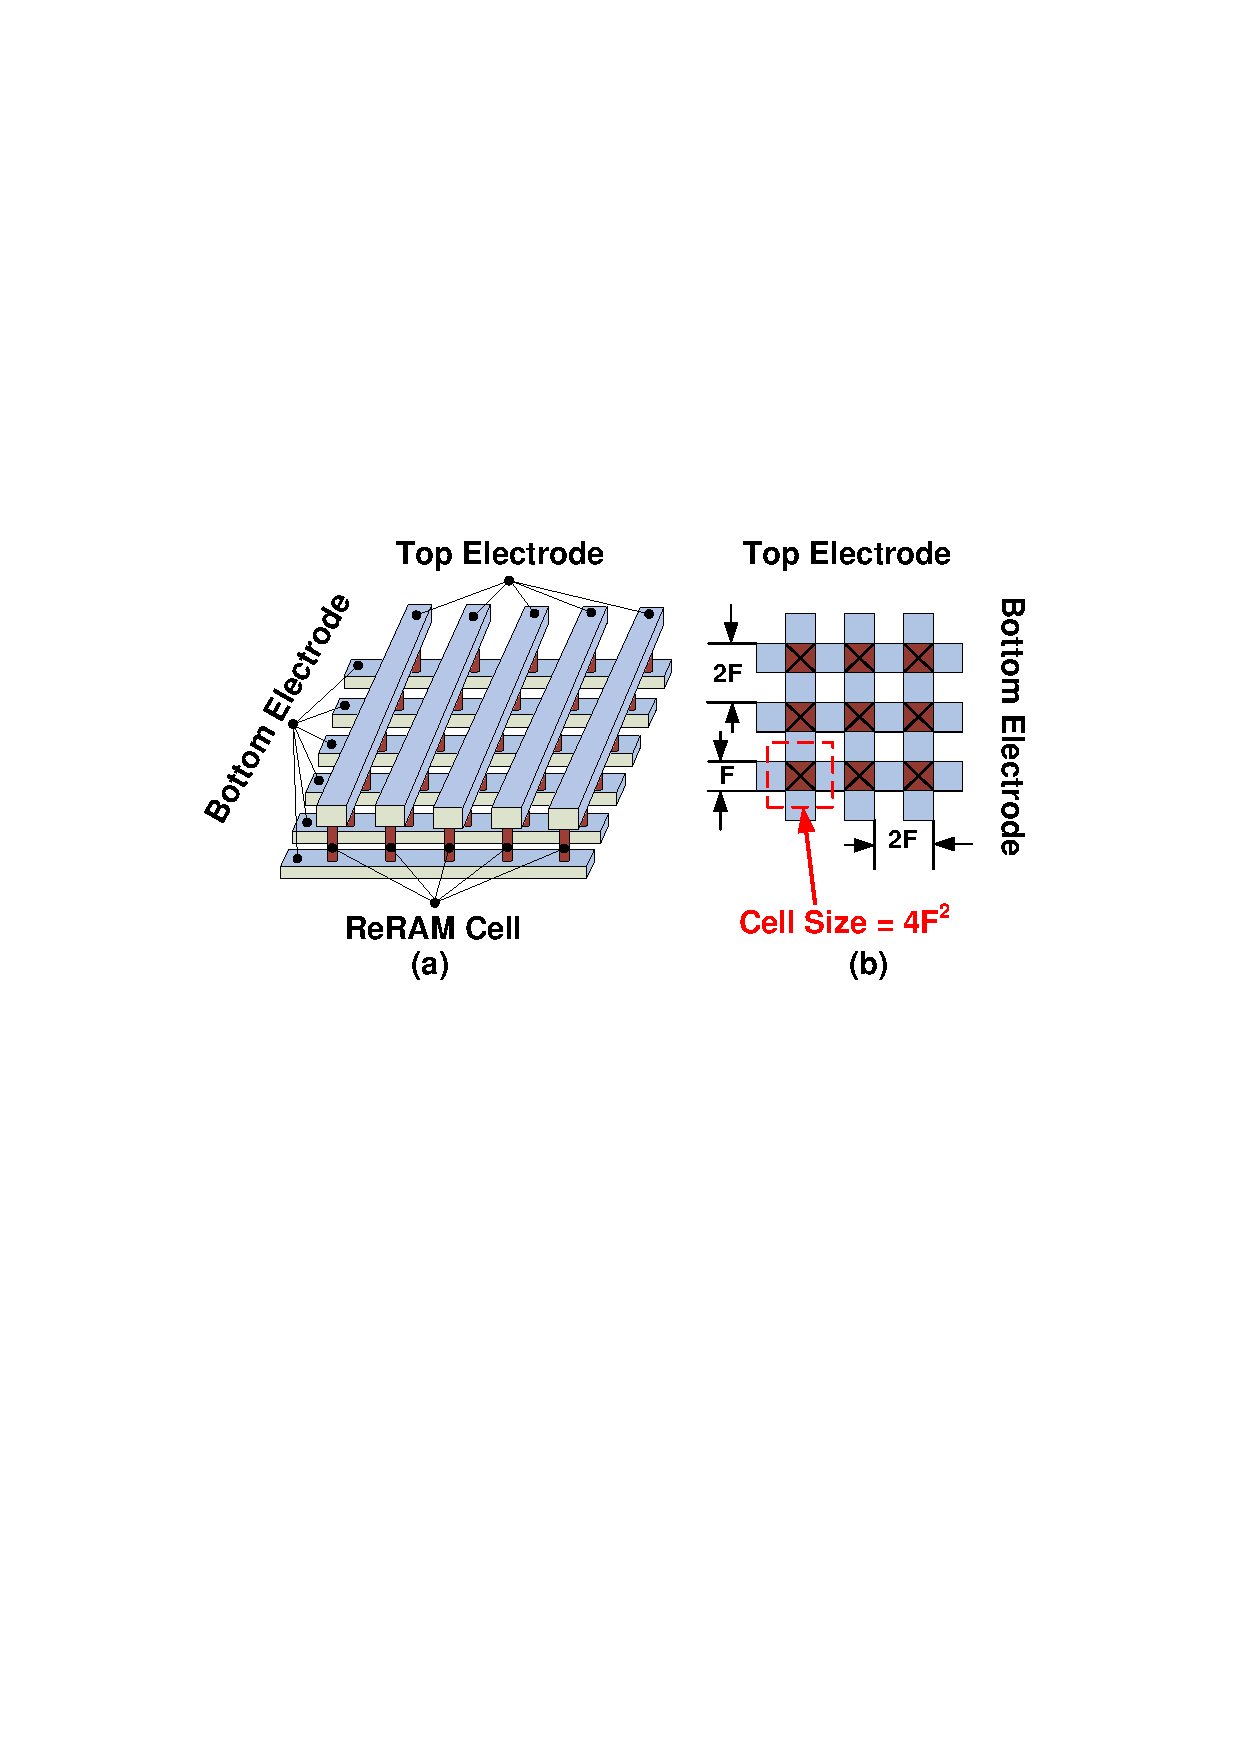
\includegraphics[width=0.45\textwidth]{./figures/crossbar_array2.pdf}\\\vspace{-10pt}
  \caption{A schematic view of a typical cross-point array. (a) The perspective of the cross-point array.
  (b) The top view of the array, from which we can clearly see that the size of each cell is $4F^2$. }\label{fig:array}
\vspace{-12pt}
\end{figure}

There are several write/read schemes for cross-point ReRAM arrays. For
example, the write operation can write either a single-bit per access or
several bits attached to the same wordline at the same time. Although the second
scheme has higher bandwidth, it requires a two-step write operation to
prevent unintentional writing~\cite{memristor:Cong}, which significantly
increases the write latency.
%Therefore, the write latency for the multi bit write operation is much larger than the one bit operation.
Furthermore, while writing to a cross-point array, the unselected wordlines
and bitlines can be either left floating or half-biased. In contrast, while reading 
a cell, the selected wordline should be biased with a read
voltage and all the other wordlines and bitlines in the array are shunted
to ground. The current in each bitline is then sensed and compared to a
reference current to determine the cell content. However, due to the sneak
current existing in the cross-point array, the current in bitlines also
varies depending upon the data patterns of unselected cells.
%is impacted significantly by the data pattern of the unselected cells in the array.
This read disturbance restricts the size of a cross-point array, since
sneak current increases as the number of cells attached to wordlines and
bitlines increases. Therefore, a cross-point array should be sized such
that the current difference of the selected cell at HRS and LRS is large
enough for reliable sensing. In addition to all of these write/read
schemes, different cell parameters will also impact the reliability,
energy consumption, and area efficiency of the cross-point ReRAM array. In
this case, it is not straightforward for a designer to figure out how to
design a workable memory array with the minimum energy consumption and
area overheads. Thus, the following sections will propose a worst-case
oriented methodology to help designers make decisions early in the
design flow.

%Depending upon the read/write scheme, the size of the array can vary significantly. In this work, we propose a methodology to find the minimum array size that meets specific energy and area constraints based on the worst-case state of the array. This will help designers find an optimal memory organization early in the design flow. %t read/write schemes as well as array sizes can be chosen for the cross-point array, it is not straightforward to figure out how to design a workable memory array with the minimum energy consumption and area overheads. Thus, following sections will proposed a worst-case oriented methodology to help designer make the decision early in the design flow.


%\subsection{Limitations of Cross-Point Architecture}
%\subsection{Related Work and Motivations}
%Although the cross-point structure can provide the fabricate simplicity and area efficiency, it also incur lots of design challenges. Many of the design challenges, such as the array size, resistance ratio as well as the data pattern have been presented and analyzed by previous researches. However, all of these researches focus on the cross point array itself and do not take into account the area or energy overhead of the peripheral circuit. Besides, a comprehensive study on different write/read schemes is also lacking. In this
%
%
%One of the well known design challenge of cross-point is the sneak path existed in the memory array, which will lead a read failure during the read operation and bring in extra energy consumption. Besides, there are also several design options can be chose during the system design. Following shows an example, which shows part of the design challenges of the cross-point structure motivates the work in this paper.
%\begin{enumerate}
%  \item \textbf{Example of the Design Challenges of Cross-Point Structure.}\\
%  In order to
%
%\begin{figure}
%\centering
%  % Requires \usepackage{graphicx}
%  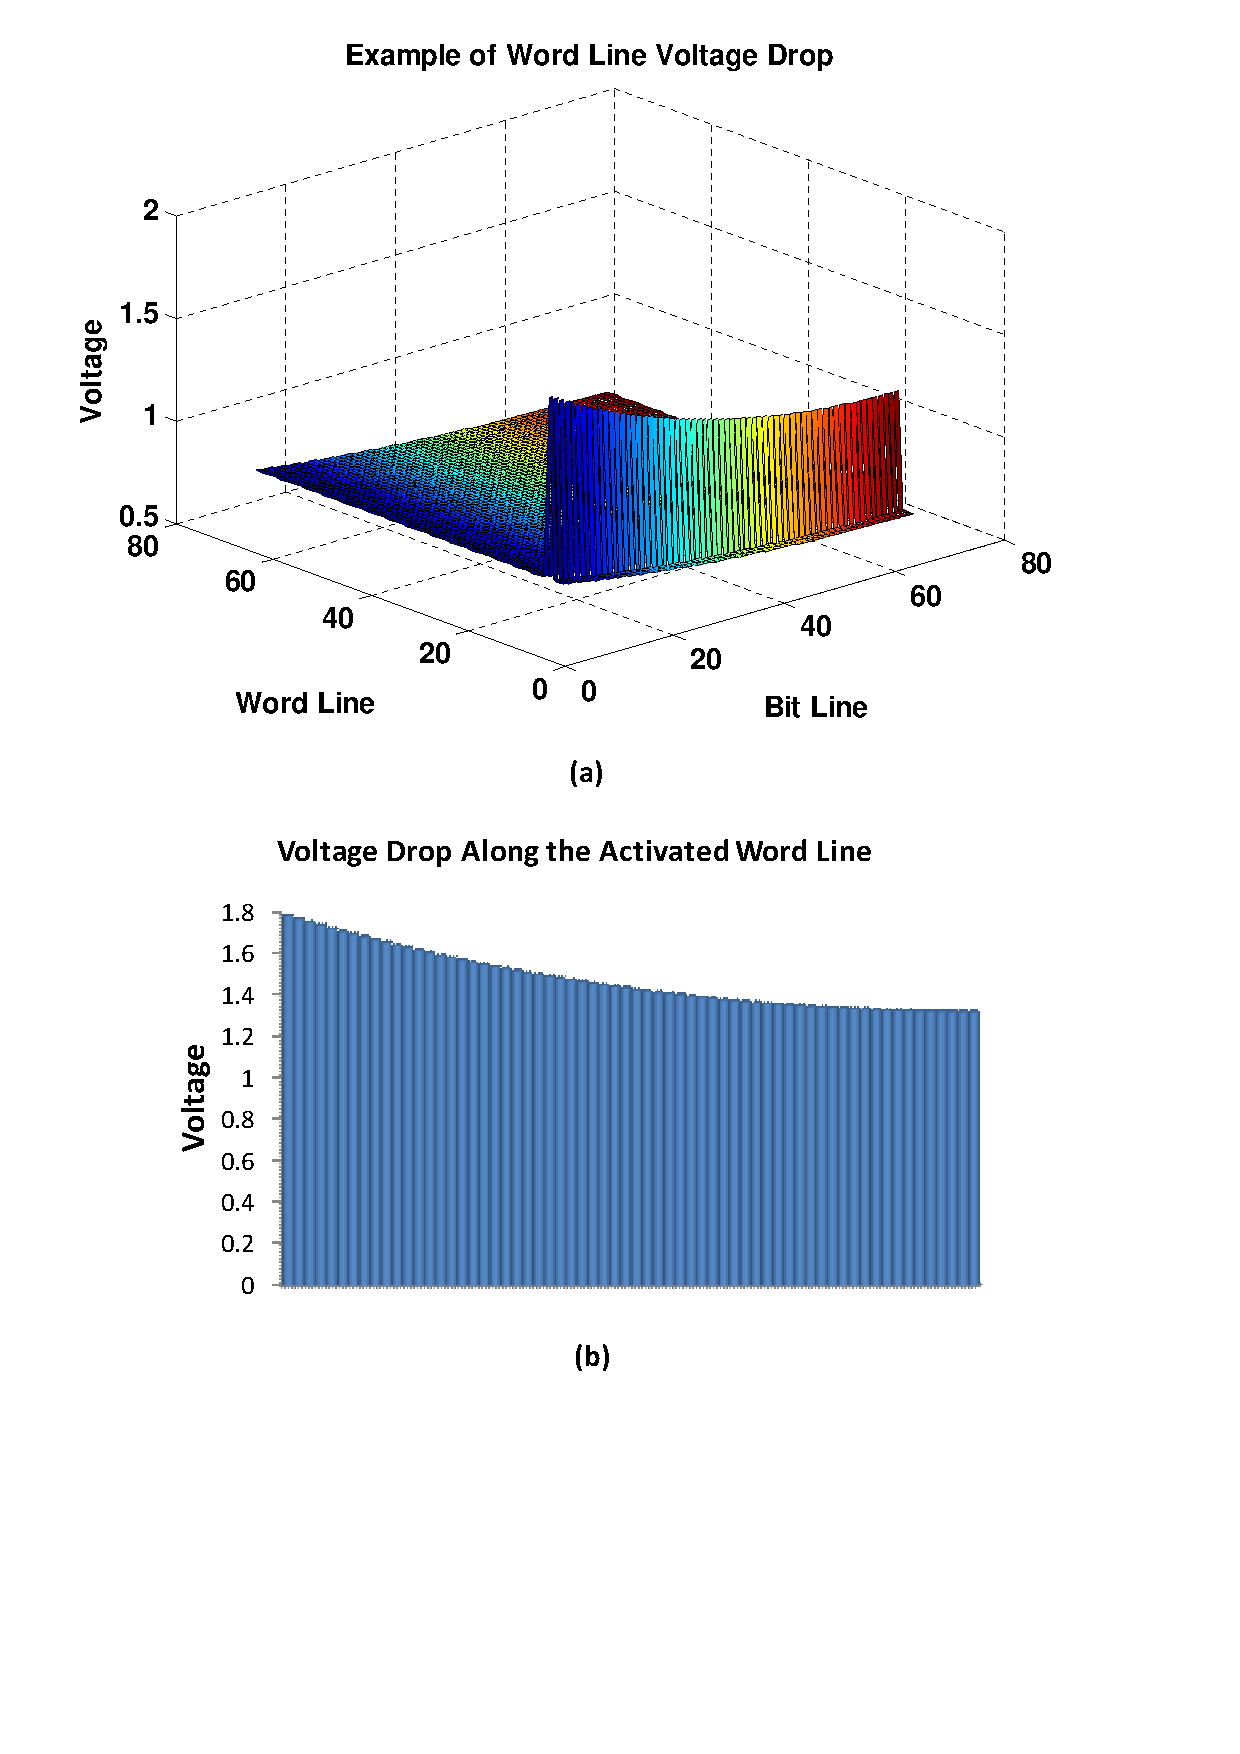
\includegraphics[width=0.4\textwidth]{./figures/example1_large.pdf}\\
%  \caption{Case 1: Voltage Drop Along the Word Line during Write Operation.}\label{fig:exampl1}
%\end{figure}
%
%  \item \textbf{Read Margin Disturbance}\\
%  123
%  \item \textbf{Energy Waste Due to Sneak Pass}\\
%  123
%\end{enumerate}
%
%~\cite{crossbar_NANO08_Nauenheim}~\cite{memristor:analog}~\cite{moore}
%

%\vspace{10pt}
\section{Related Work}\label{sec:related}
 
%\vspace{10pt}
\section{Modeling of the Cross-Point Memory}\label{sec:model}

%In this section, we present a detailed mathematical model for cross-point
%arrays. By using this model, along with specific parameters and edge
%conditions, the reliability, energy consumption, and area overheads of
%different read/write schemes can be easily evaluated.

%\subsection{Basic model of Cross-Point Memory}
The basic circuit model of an $M$ by $N$ cross-point ReRAM array is shown
in Figure~\ref{fig:modeling}. The model is built upon Kirchhoff's Current
Law (KCL) and its validity can be guaranteed by deductions from the basic
circuit theory. The horizontal lines are wordlines and vertical lines
represent bitlines. The ReRAM cells are located at each cross-point of
wordline and bitlines. The resistance of the ReRAM cell at the cross-point
of $i^{th}$ wordline and $j^{th}$ bitline is represented by $R_{i,j}$. We
assume the resistance of the wire connecting two cross-points to be
$R_{line}$. The input resistance of each wordline and bitline is $R_v$ and
the resistance of sense amplifier is $R_s$. In order to set up the KCL
equations, the voltage at each cross-point is indicated as $V_{i,j}$ for
wordline and $V'_{i,j}$ for bitline. A detailed cross-point is also shown
in Figure~\ref{fig:modeling}(b). The input voltage for the $i^{th}$
wordline is $V_{Wi}$ and the $i^{th}$ bitline is $V_{Bi}$. In the case
where a wordline takes input from both the sides, the voltage at the other
end of the $i^{th}$ wordline is represented as $V'_{Wi}$.
%Finally, the voltage at the sense amplifier is $V'_{Bi}$ during the read operation.
%YOU MIGHT WANT TO CHANGE THE ABOVE PARA INTO A TABLE

\begin{figure}%[!hb]
\centering
  % Requires \usepackage{graphicx}
  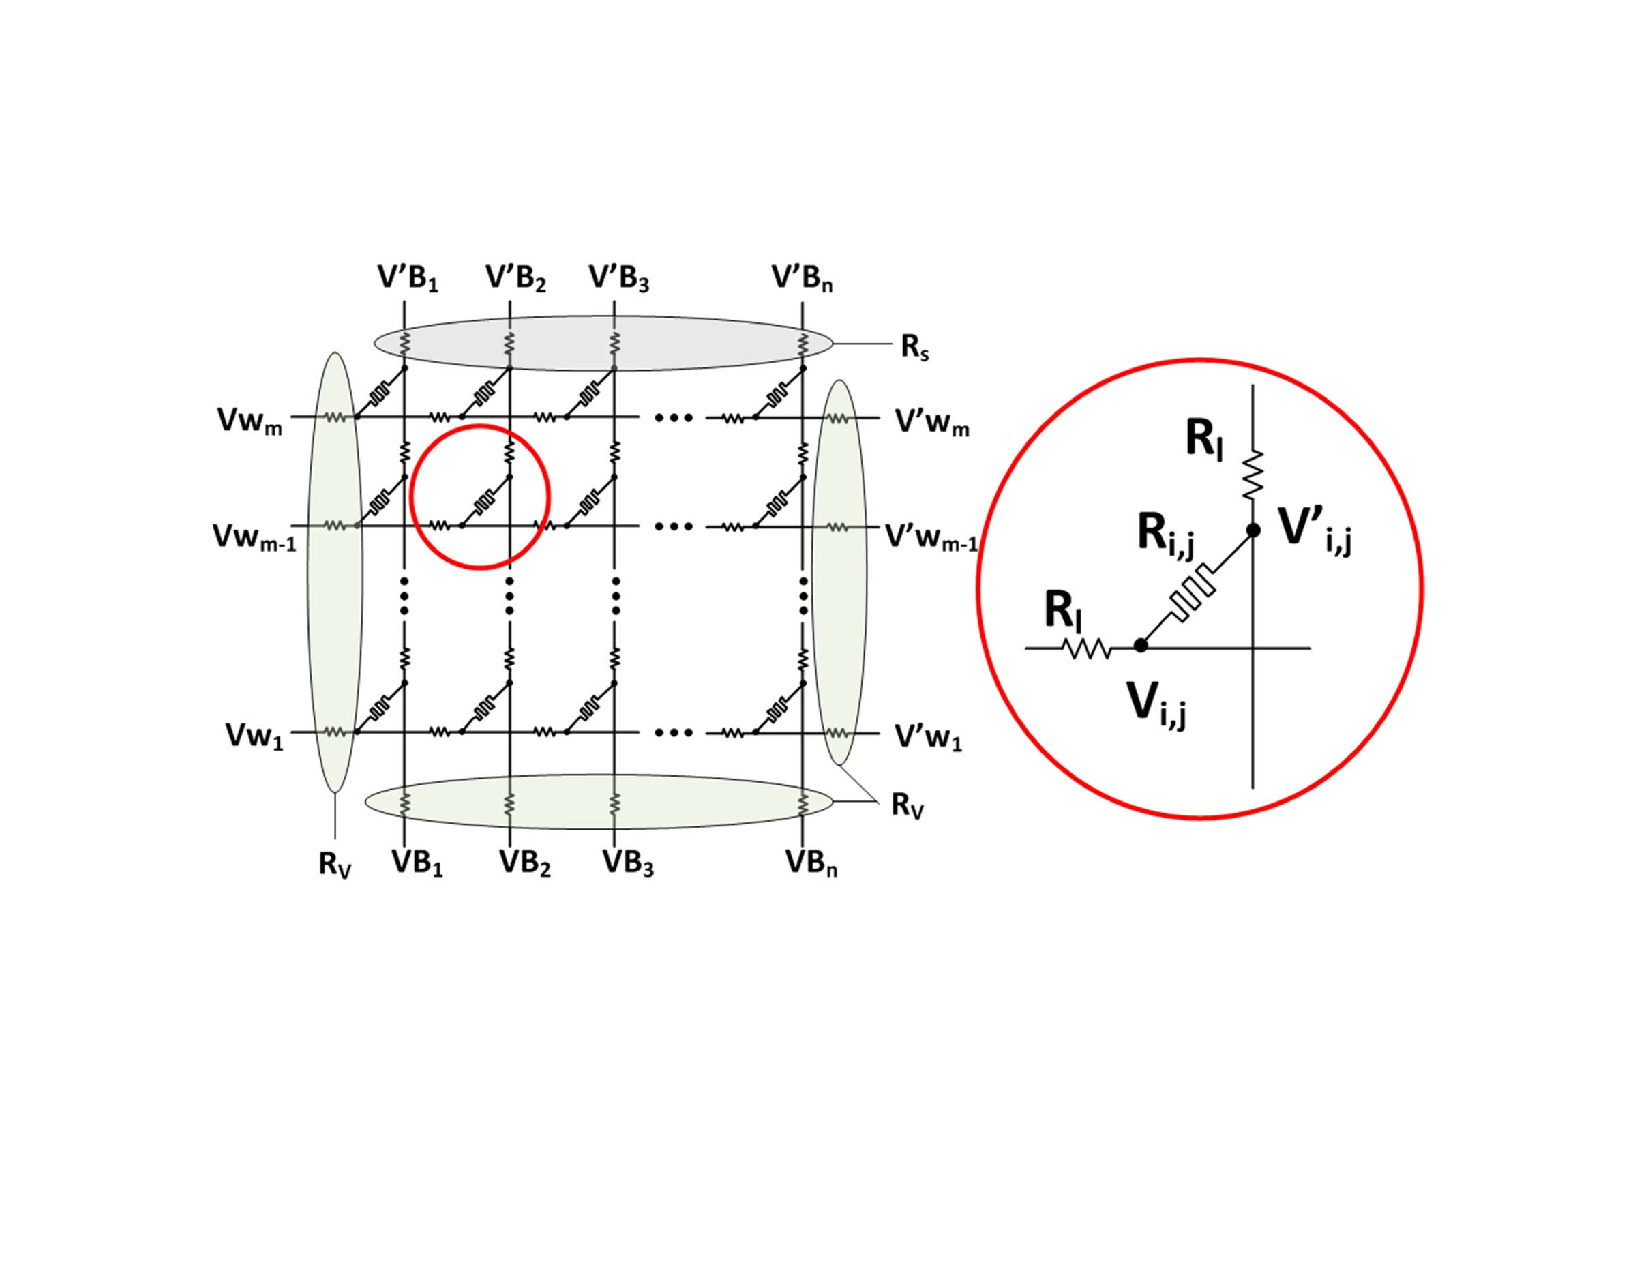
\includegraphics[width=0.45\textwidth]{./figures/model_f.pdf}\\
  \caption{The basic model of typical cross-point array.}\label{fig:modeling}
  \vspace{-12pt}
\end{figure}

%\subsection{Mathematical Model of a Cross-Point Array}
Based on this model, the current equations for each cross-point can be set
following KCL: $ {\Sigma}_{I=1}^kI_k=0.$ All of the cross-points have
similar structure with no more than three current branches and therefore
it is very easy to set up the KCL equations for each cross-point. However,
we should treat the cross-points at the edges of the array specifically
because KCL equations for these cross-points vary with different
write/read schemes. For example, the unselected wordline for write
operation can be either half biased or left floating. Thus, the edge
conditions should be adjusted according to each write/read scheme. In
particular, all of the cross-points in an array can be classified into
three major categories: \emph{normal point}, \emph{activated point} and
\emph{floating point}.

The normal points are located inside the memory array. In other words, for
all of the nodes with $1<i<m$ and $1<j<n$, the KCL equations take the form
of
\begin{equation}\label{equ:KCL1}
R_l^{-1}V_{i,j-1} -(2R_l^{-1}+R_{i,j}^{-1})V_{i,j}+ R_l^{-1}V_{i,j+1}+R_{i,j}^{-1}V'_{i,j}=0,
\end{equation}
for the node at wordline layer and
\begin{equation}\label{equ:KCL2}
R_l^{-1}V'_{i-1,j} -(2R_l^{-1}+R_{i,j}^{-1})V'_{i,j}+ R_l^{-1}V'_{i+1,j}+R_{i,j}^{-1}V_{i,j}=0,
\end{equation}
for the node at bitline layer.

The activated point and floating point represent the nodes at the edge of
cross-point array with different conditions: an edge point, which is
directly connected to the voltage input or to the ground, can be
considered as an activated point. Otherwise, it is a floating point. For
example, consider the point located at the intersection of $i^{th}$
wordline and $1^{st}$ bitline. If the $i^{th}$ wordline is activated by an
input voltage of $V_{Wi}$, this cross-point is an activated point, and the
KCL equation for this point is:
\begin{equation}\label{equ:KCL3}
-(R_v^{-1}+R_l^{-1}+R_{i,1}^{-1})V_{i,1}+ R_l^{-1}V_{i,2}+R_{i,1}^{-1}V'_{i,1}=-R_v^{-1}V_{Wi}.
\end{equation}
Otherwise, it is floating and its KCL equation is
\begin{equation}\label{equ:KCL4}
-(R_l^{-1}+R_{i,1}^{-1})V_{i,1}+ R_l^{-1}V_{i,2}+R_{i,1}^{-1}V'_{i,1}=0.
\end{equation}

For clarity, a ${2mn\times 1}$ vector ${V}$ is defined to represent all of the variables in the KCL equations:
\begin{equation}\label{equ:V1}
{V}=[{V_1}^T,{V_2}^T...{V_m}^T,{V'_1}^T,{V'_2}^T...{V'_m}^T]^T,
\end{equation}
where,
%\begin{equation}\label{equ:V2}
%{V_i} = [V_{i,1},V_{i,2}...V_{i,n}]^T,\\
%\end{equation}
%\begin{equation}\label{equ:V3}
%{V'_i} = [V'_{i,1},V'_{i,2}...V'_{i,n}]^T,
%\end{equation}
\begin{equation}\label{equ:V2}
{V_i} = [V_{i,1},V_{i,2}...V_{i,n}]^T,~~{V'_i} = [V'_{i,1},V'_{i,2}...V'_{i,n}]^T,
\end{equation}
for $i=1,2...m$. Then all of the KCL equations can be considered as a
system of linear equations, which has the form
\begin{equation}\label{equ:matrix}
A\cdot V = C.
\end{equation}
$A$ is a ${2mn\times{2mn}}$ coefficient matrix, which is determined by
Equations(\ref{equ:KCL1})-(\ref{equ:KCL4}). $C$ is a ${2mn\times{1}}$
vector, containing the constant terms of these equations. As shown, all of
the KCL equations have simple structure and are similar to each
other. Therefore, the linear equation system has a relatively fixed format
and simple structure, making it easy to establish and adjust the
coefficients and constants according to different design schemes. Besides,
due to the simplicity of the KCL equation, $A$ is populated primarily with
zeros and can be saved as a sparse matrix, which will further reduce the
storage cost during the computation.

To validate our analytical model, we compared the results with the HSPICE
simulations using a simple resistor model in cross-point memory arrays. DC
analysis was performed by HSPICE which solved the voltage of every node in
the array. The results of eight cross-point arrays with different array
size and specific data pattern are shown in Figure ??, the voltage drop on
the selected cell derived from our analytical model are consistent with the
HSPICE simulation results.
\begin{figure}%[!t]
\centering\label{fig:SPICE}
  % Requires \usepackage{graphicx}
  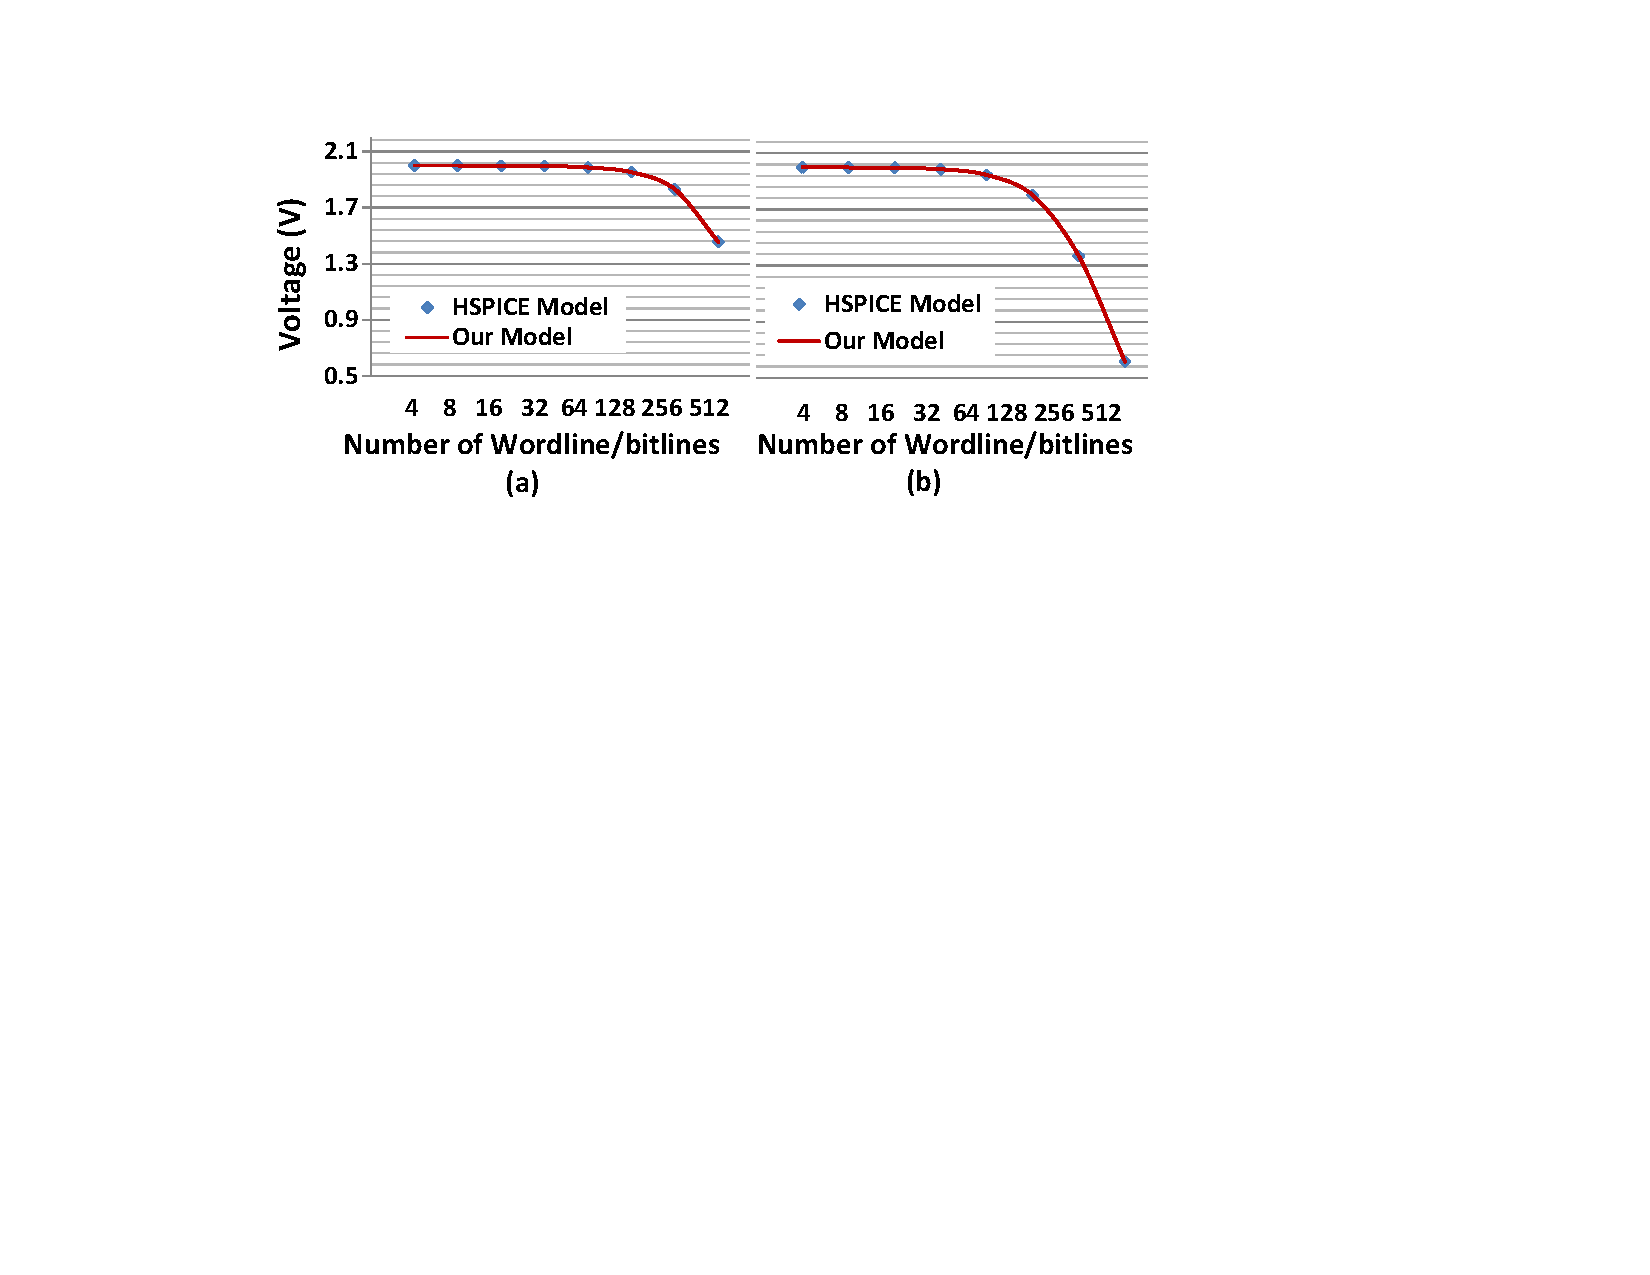
\includegraphics[width=0.5\textwidth]{./figures/SPICE.pdf}\\
  \caption{Analytical model verification of voltage drop comparing to HSPICE simulations (a) with non-linearity of 5; (b) without non-linearity.}\label{fig:reliable_region}
    \vspace{-10pt}
\end{figure}
%
%The characteristics of the linear system can be summarized as:
%\begin{enumerate}
%  \item
%  As shown in Equation~(\ref{equ:blockedmatrix}), the coefficient matrix $A$ can be further partitioned into 4 smaller subblocks :
%    \begin{equation}\label{equ:blockedmatrix}
%        \mathbf{A} = \left[
%        \begin{array}{cc}
%            A1 & A2  \\
%            A3 & A4  \\
%        \end{array} \right].
%    \end{equation}
%All of these subblocks have the same size of $m\times n$. Subblock
%$A2$ and $A3$ are diagonal matrixes and have the value of: $A2_{i,i} =
%A3_{i,i} = R_{i,i}^{-1}$. $A2$ and $A3$ do not change their values
%with different schemas. However, $A1$ and $A4$ are a little more
%complex than $A2$ and $A3$. $A1$ is a tridiagonal matrix and has
%nonzero elements only in the main diagonal, and the first line below
%and above the diagonal. Similarly, $A_4$ is a special tridiagonal
%matrix, which has nonzero elements in the main diagonal, and the
%$n^{th}$ line below and above the diagonal, where $n$ is the number of
%bitline in the cross-point model. The value of the elements in $A1$
%and $A4$ can be easily derived from Equation (\ref{equ:KCL1}) and
%(\ref{equ:KCL2}). However, the edge condition varies with different
%program schemes. Therefore, the coefficients related to the edge
%condition should be set according to the program schemes. Clearly, the
%four edges shown in Figure~\ref{fig:modeling} correspond to different
%coefficients in $A1$ and $A4$. Due to the space limitations, we
%consider the nodes at the left edge of the array as an example. A
%similar procedure can be followed to initiate the coefficients of
%other edge. The coefficients of nodes at the left edge of the array
%($V_{i,1}$) can be set as:
%
%    \begin{equation}
%    A1(k,k) = \left\{
%    \begin{array}{ll}
%    -(R_l^{-1}+R_{i,1}^{-1})   & \text{if } floating\\
%    -(R_v^{-1}+R_l^{-1}+R_{i,1}^{-1})& \text{if } activated
%    \end{array} \right.
%    \end{equation}
%    where $k=(n-1)i+1$ for $i=1,2...m$.
%
%  \item The constant terms $C$ is a $2mn{\times}1$ vector. Equation(\ref{equ:KCL1})-(\ref{equ:KCL4}) show that only KCL equations of the activated points have constant terms. Therefore, only the following elements in $C$ may have non-zero value: $C((i-1)n+1)$, $C(in)$, $C(mn+i)$ and $C((2m-1)n+i)$ for $i=1,2...m$, corresponding to the nodes at the four edges respectively. Likewise, as an example, we consider nodes $V_{i,1}$. The constant corresponding to these nodes can be defined as:
%    \begin{equation}
%    C((i-1)n+1) = \left\{
%    \begin{array}{ll}
%    0   & \text{if } floating\\
%    -R_v^{-1}V_{Wi}& \text{if } activated
%    \end{array} \right.
%    \end{equation}
%\end{enumerate}
Thus, with parameters such as the resistance of ReRAM cells, the
resistance of interconnect wires, program voltages, and write/read
schemes, voltages at various cross points can be obtained by solving the
system of linear equations. With detailed voltage values,
$V_{2mn{\times}1}$, we can analyze the array at a fine granularity. These
values are also critical to evaluate reliability, energy consumption,
driven current density, and area overheads of a cross-point array.

\vspace{-4pt}
\section{Analysis of Design Constraints - A Case Study}\label{sec:w_and_r}

In this section, we study the effect of various schemes on cross-point
size and reliability in detail by using our mathematical model. The
constraints on array size, energy consumption and area overhead are
analyzed in the worst cases scenario. The results of this study will be a
useful guide in designing a cross-point array.

\vspace{-10pt}
\subsection{Overview}
%As shown in Figure~\ref{fig:modeling}, i
In order to write or read a cross-point array, proper voltages should be
applied across the ReRAM cell. Although the goal of a read operation is
different from a write operation, both of them are realized by fully
biasing the selected wordlines/bitlines and floating (or half biasing)
unselected wordlines/bitlines. Thus, the coefficient matrix $A$ and the
constant vector $C$ are very similar for both. In addition, their energy
consumption and area overhead will also have a similar trend. Therefore,
in this section, we first study the write operation comprehensively. After
that, for read operation, we mainly focus on the read margin analysis
since it is unique to read operations.
%can be very useful to guide the design of the cross-point array.
%Also, we assumes that the in the case of worst scenario, the ReRAM cells at the selected wordline, th
%Since it is impossible to consider all of the data pattern stored in the array,

Table~\ref{table:parameter} shows the circuit parameters of our baseline
50nm design. The data is derived from the recently published studies on
ReRAM~\cite{ReRAM_overview,memristor:Cong,ReRAM_Renesas}. The
non-linearity coefficient is defined as: $K_r(p,V) = p \times
R(V/p)/R(V)$, where $R(V/p)$ and $R(V)$ are the equivalent resistance of
the cell biased at $V/p$ and $V$~\cite{memristor:Cong}. Therefore, the
resistance of a ReRAM cell with non-linearity is not constant but varies
with the applied voltage. By using these parameters, we study reliability,
energy consumption, and area overheads for four different write schemes,
and discuss the sensitivities of these schemes to the data pattern of HRS
and LRS ReRAM cells and cell non-linearity. In this section, the baseline
design uses the cell with write current of $40 uA$ and non-linearity
$Kr=20$.

\begin{table}[!b]
  \centering
  \scriptsize
    \scriptsize
  \caption{Parameters of the baseline Cross-Point Array}\label{table:parameter}
  \vspace{-5pt}
%  \begin{tabular}{|cccccp{3.5cm}|}
  \begin{tabular}{c|c|c}
    \hline    \hline
    % after \\: \hline or \cline{col1-col2} \cline{col3-col4} ...
    \textbf{Metric} & \textbf{Description} & \textbf{Typical Values (Range)} \\
    \hline
    \textbf{$A_{cell}$} & Cell Size & \textbf{$4F^2$} \\
    \textbf{$R_l$} &  Interconnection Resistance&\textbf{$0.65\Omega$} \\
    \textbf{$V_{RESET}$} & Threshold voltage for RESET&\textbf{$2.0V$} \\
    \textbf{$V_{SET}$} & Threshold voltage for SET&\textbf{$-2.0V$} \\
    \textbf{$V_{READ}$} & Read Voltage of Cell&\textbf{$0.5V$} \\
    \textbf{$I_{on}$} & Write Current for LRS Cell &\textbf{$40uA$~~($20\sim200uA$)} \\
    \textbf{$V_{W}(R)$} & Wordline Voltage during Read &\textbf{$0.5V$} \\
    \textbf{$V_{W}(W)$} & Wordline Voltage during Write  &\textbf{$\pm2V$} \\
    \textbf{$V_{W}(H)$} & Half Selected wordline Voltage &\textbf{$1V$} \\
    \textbf{$V_{B}(R)$} & Bitline Voltage during Read  &\textbf{$0V$} \\
    \textbf{$V_{B}(W)$} & Bitline Voltage during Write  &\textbf{$0V$} \\
    \textbf{$V_{B}(H)$} & Half Selected bitline Voltage &\textbf{$1V$} \\
    \textbf{$K_r$} & Nonlinearity of ReRAM Cell &\textbf{$20$~~($2\sim40$)} \\
    \textbf{$M,N$} & Number of wordlines/bitlines &\textbf{$512$~~($8\sim1024$)} \\
    \hline
  \end{tabular}
  \vspace{-10pt}
\end{table}

\subsection{Write Operation}
To write a ReRAM cell, an external voltage is applied across the cell for
a certain duration. Intuitively, there are four possible schemes for the
write operation:
\begin{enumerate}
  \item According to the location of a selected cell, activate one
      wordline and one bitline and leave all of other lines floating
      (FWFB scheme).
  \item Activate the selected wordline and bitline. Leave all the
      unselected wordlines floating and half bias the unselected
      bitlines (FWHB scheme).
  \item In contrast to the scheme 2), activate the selected wordline
      and bitline. Leave all the unselected bitlines floating and half
      bias the unselected wold lines (HWFB scheme).
  \item Activate the selected wordline and bitline. Then half bias the
      unselected wordlines and bitlines (HWHB scheme).
\end{enumerate}
However,the FWFB scheme has inherent problem that may result in severe
write disturbance~\cite{crossbar_NANO2003_Ziegler}. Therefore, in the
following discussion, we only compare the results between FWHB, HWFB and
HWHB schemes. For each of these three schemes, we can either write several
cells at one wordline at the same time or write only one bit per access
and distribute the write operation to several arrays. In the following
discussion, we start from one bit per access write operation, then the
results of one wordline per access method are discussed.

%Since several potential read/write schemes can be used to program a memory array, it is difficult to identify the ideal scheme that meets the design constraints in terms of area, energy, and reliability.
%However, the FWFB scheme has inherent problem that may result in severe
%write disturbance. For example, for writing a ReRAM cell located at the
%cross point of the $i^{nd}$ wordline and the $j^{nd}$ bitline in a $M
%\times N$ matrix ($M>N$), the worst case voltage drop of unselected cells
%appears when all of the ReRAM cells at the selected bitline are in the
%HRS, while all of the other cells are in the LRS. In this case, the
%voltage drop across the selected cell almost has the same magnitude as the
%unselected cell at the same bitline, resulting the write disturbance to
%all of the unselected cells at the selected bitline. Actually, the worst
%case voltage drop of the unselected cell can be calculated as:
%\begin{equation}\label{worst_FWFB}
%V_{worst}=V_{select} \cdot [1-\frac{1}{M+(N-1)R_{off}/R_{on}}].
%\end{equation}
%Considering that the reported On-OFF resistance ratio of ReRAM cell is
%always $>50$
%~\cite{ReRAM_IEDM2010_Ho,ReRAM_IEDM2010_Chien,ReRAM_IEDM2010_Lee_Diode,ReRAM_IEDM2010_Lee_Evidence,ReRAM_ISSCC2011_Sheu,ReRAM_ISSCC2011_Otsuka},
%, the worst case voltage drop at the unselected cell is larger than $98\%$
%of the voltage at the selected cell, making it is impossible to build a
%reliable cross-point structure ReRAM with the FWFB scheme. Therefore, in
%the following discussion, we only compare the results of FWHB, HWFB and
%HWHB schemes. For each of these three schemes, we can either write several
%cells at one wordline at the same time or only write one bit per access
%and distribute the write operation to several arrays. In the following
%discussion, we start from one bit per access write operation, then the
%results of one wordline per access method are discussed.

%Since reliability, energy consumption, and area overheads for these
%schemes are different, we address these problems separately and finally
%combine all constraints to provide design guidelines for write operations.


\vspace{6pt} \emph{Reliable Write Operation.} \vspace{6pt}

Write reliability is a serious concern in cross-point arrays. In an ideal
condition, the resistance of wires and the sneak currents in unselected
cells are negligible. In such a scenario, all the write schemes discussed
above will make sure that the write voltage $V_W(W)-V_B(W)$ is fully
applied across the specified cell. However, in reality, both wire
resistance and sneak current are non-trivial. Hence, the operation of
cross-point array varies based on the data pattern stored in ReRAM cells.
A write is considered reliable if it modifies the content of the selected
cells to the new value without disturbing other unselected cells.
%A reliable write operation can be defined as: switching the selected cells into required states without disturbing the states of unselected cells.
Correspondingly, there are two potential problems with writes: \emph{write
failure}, an unsuccessful write on selected cell, and \emph{write
disturbance}, an undesirable write on unselected cell. It is necessary to
ensure that a write scheme guarantees reliable operation even in the worst
case (w.r.t the location of cells to written and the data pattern stored
in the cross-point array). Otherwise, after several unreliable write
operations, the data stored in the cross-point array will become
unpredictable.

%We first use an example to show the problem with FWFB scheme, which may
%result in severe write disturbance. Figure~\ref{fig:FWFR} shows the
%voltage drop across each ReRAM cell of a $64 \times 64$ cross-point array.
%In this example, in order to write the cell at the cross point of the
%$32^{nd}$ wordline and the $32^{nd}$ bitline, the selected wordline and
%bitline are biased at 2V and 0V, respectively. All of the other wordlines
%and bitlines are left floating. The ReRAM cells at the selected bitline are
%in the HRS, while all of the other cells are in the LRS. It is clear that
%the voltage drop across the selected cell ($V_{32,32}$) almost has the
%same magnitude as the unselected cell at the same bitline, resulting the
%write disturbance to all of the unselected cells at the selected bitline.
%Actually, for a $M \times N$ matrix ($M>N$), the worst case voltage drop
%of the unselected cell can be calculated as:
%\begin{equation}\label{worst_FWFB}
%V_{worst}=V_{select} \cdot [1-\frac{1}{M+(N-1)R_{off}/R_{on}}].
%\end{equation}
%
%\begin{figure}[!b]
%\centering
%  % Requires \usepackage{graphicx}
%  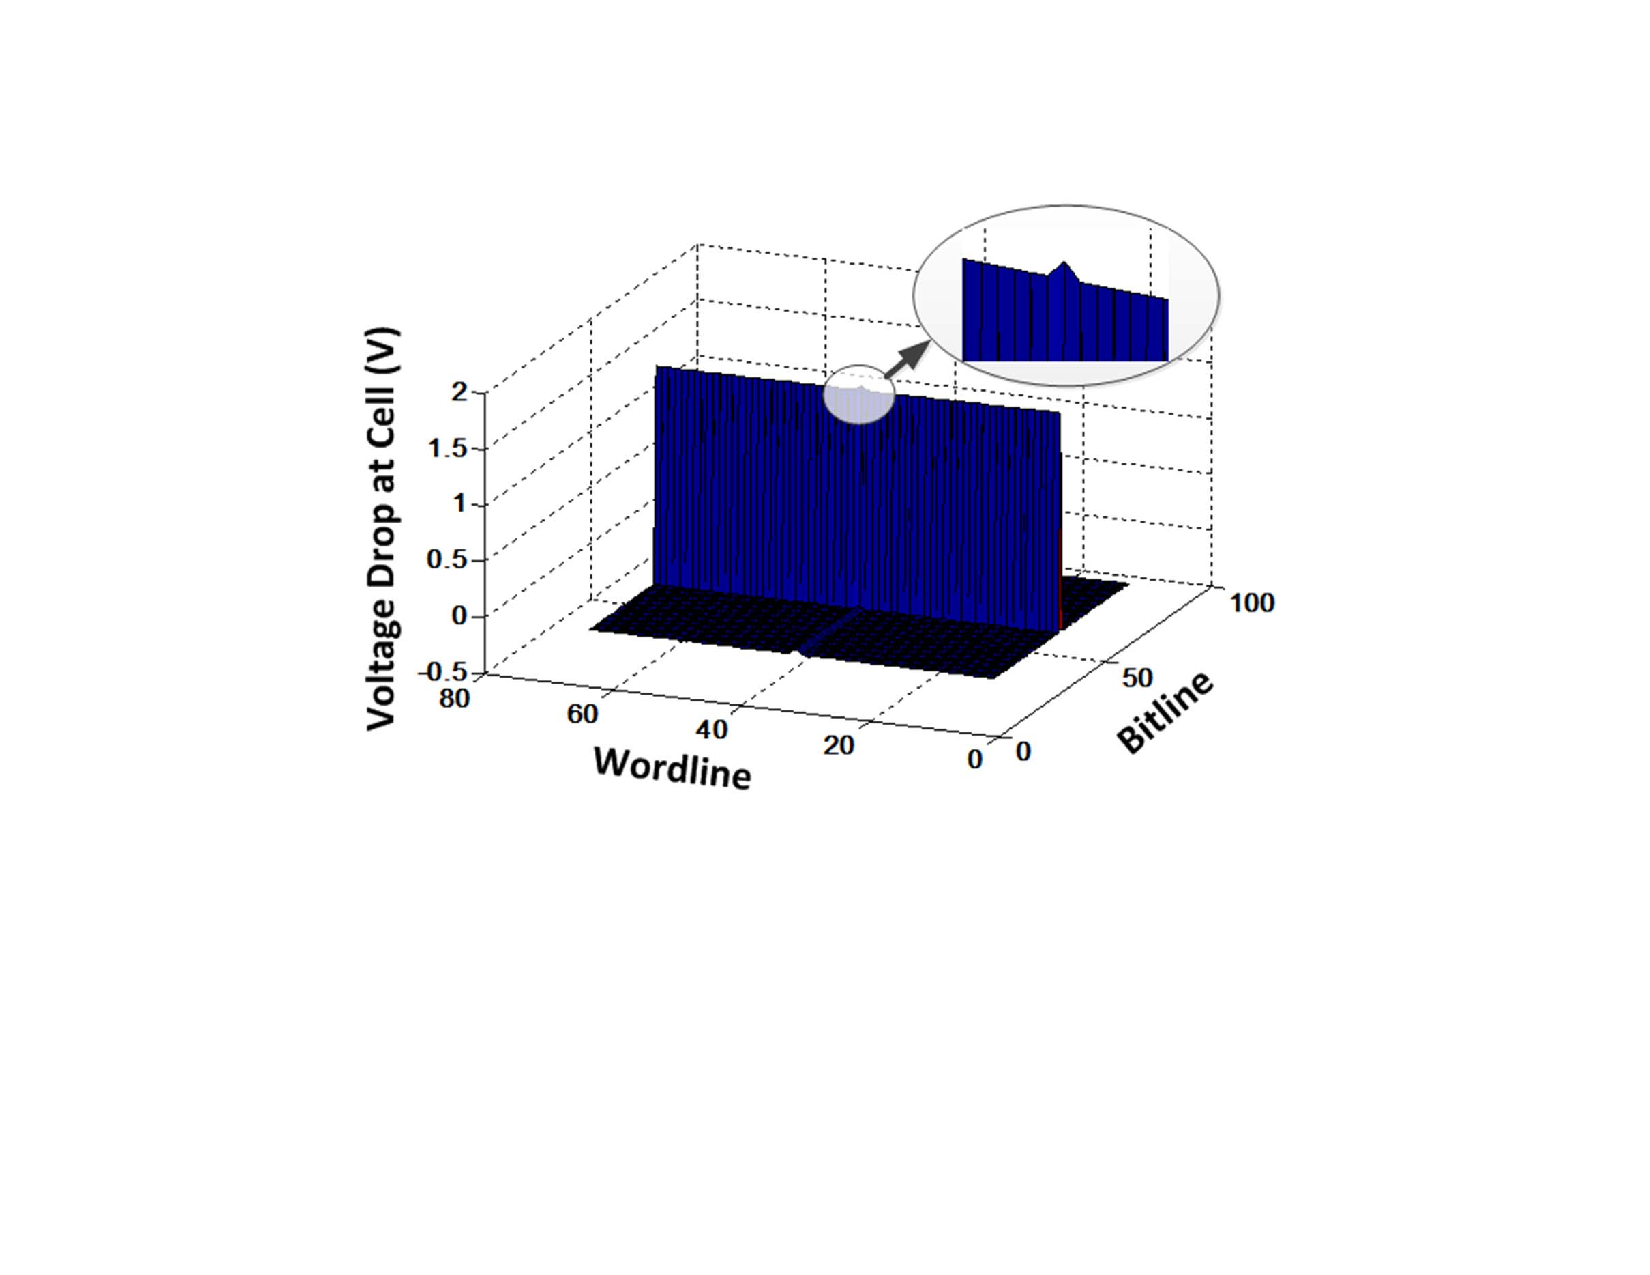
\includegraphics[width=0.4\textwidth]{./figures/FWFB_f.pdf}\\
%  \caption{Write disturbance for FWFB schemes. ( $V_{W32} = 2V$, $V_{B32} = 0V$. $R_{x,32}$ at HRS, others at LRS.) }\label{fig:FWFR}
%\end{figure}
%Considering that the reported On-OFF resistance ratio of
%ReRAM cell is always $>50$ ~\cite{ReRAM_IEDM2010_Ho,ReRAM_IEDM2010_Chien,ReRAM_IEDM2010_Lee_Diode,ReRAM_IEDM2010_Lee_Evidence,ReRAM_ISSCC2011_Sheu,ReRAM_ISSCC2011_Otsuka},
%, the worst case voltage drop at the unselected cell is larger than $98\%$ of the voltage at the selected cell, making it is impossible to build a reliable cross-point structure ReRAM with the FWFB scheme. Therefore, in the following discussion, we only compare the results of FWHB, HWFB and HWHB schemes. For each of these three schemes, we can either write the cells at one wordline at the same time or only write one bit per access and separate the write operation to several arrays. In the
%following discussion, we start from one bit per access write operation,
%then the results of one wordline per access method are discussed.


%as long all of unselected cells in the activated wordline (or all of unselected cells in the activated bitline) are at HRS and other cells are in LRS, the voltage drop at unselected cells are mainly applied at the HRS cells at the wordline (or bitline).
%The worse case scenario for FWFB write disturbance can be defined as: all of unselected cells in the activated wordline (or all of unselected cells in the activated bitline) are at HRS and other cells are in LRS. In this case, the voltage drop at unselected cells are mainly applied at the HRS cells at the wordline (or bitline).

Write failure typically results from the voltage drop at the interconnect
wires along the wordline and bitline. It has been shown
that~\cite{crossbar_TED_2010}, for one bit per access write operation, the
worst case voltage drop occurs when writing the cell at the cross point of
the $M^{th}$ wordline and the $N^{th}$ bitline with all of the cells in
the array are in LRS. In order to avoid the write failure and successfully
program the selected ReRAM cell, the driven voltage should be boosted to a
higher level, making sure that the voltage across the cell exceeds the
threshold voltage even at the worst case. Figure~\ref{fig:worst_v} shows
the lower bounds of the driven voltage for different sizes of cross-point
array. The minimum wordline/bitline voltage increases from 2.01~V for a
$32 \times 32$ array to nearly 7~V for a $1024 \times 1024$ cross-point
array. In addition, for a memory capability, the cross-point array can be
organized with different number of wordlines and bitlines. For example, a
256K bits cross-point array can be implemented either by a $512 \times
512$ array or by a $64 \times 4096$ array. In the latter case, the voltage
drops along the wordline will be much worse than along the bitline.
Figure~\ref{fig:shape} examines the voltage requirements for different
array organizations with different write schemes. The result shows that
from a reliability point of view, a cross-point array with same number of
wordlines and bitlines is the best choice. Furthermore, we also notice
that when the array has the same number of wordlines and bitlines, FWFB,
HWFB and FWHB schemes have the same minimum driven voltage.

%Clearly, the magnitude of the voltage drop increases with the array size and the resistance of interconnect wires.

\begin{figure}%[!hb]
\centering
\hspace{-5pt}
  % Requires \usepackage{graphicx}
  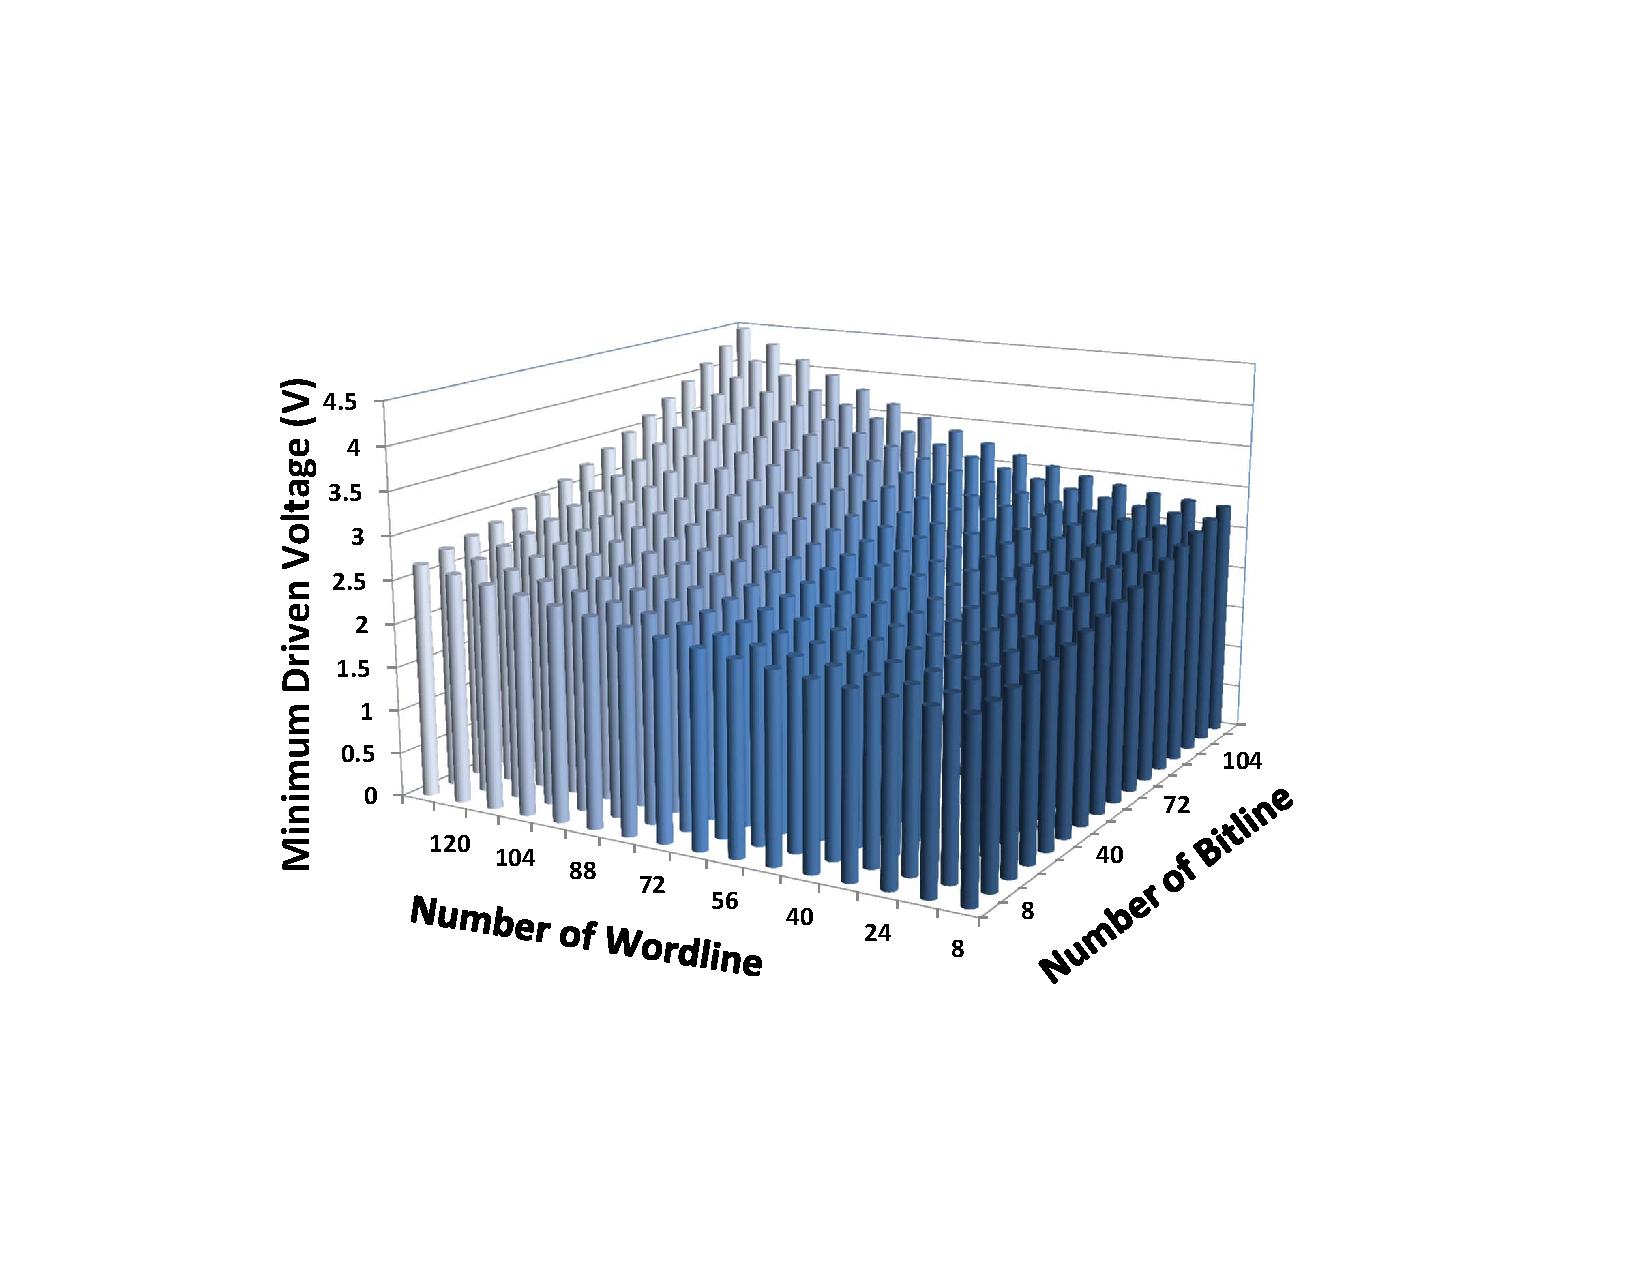
\includegraphics[width=0.45\textwidth]{./figures/worst_v_f.pdf}\\
  \caption{Required write voltages for different cross-point arrays (threshold voltage = 2V.). }\label{fig:worst_v}
  \vspace{-5pt}
\end{figure}


\begin{figure}%[!t]
\centering
  % Requires \usepackage{graphicx}
  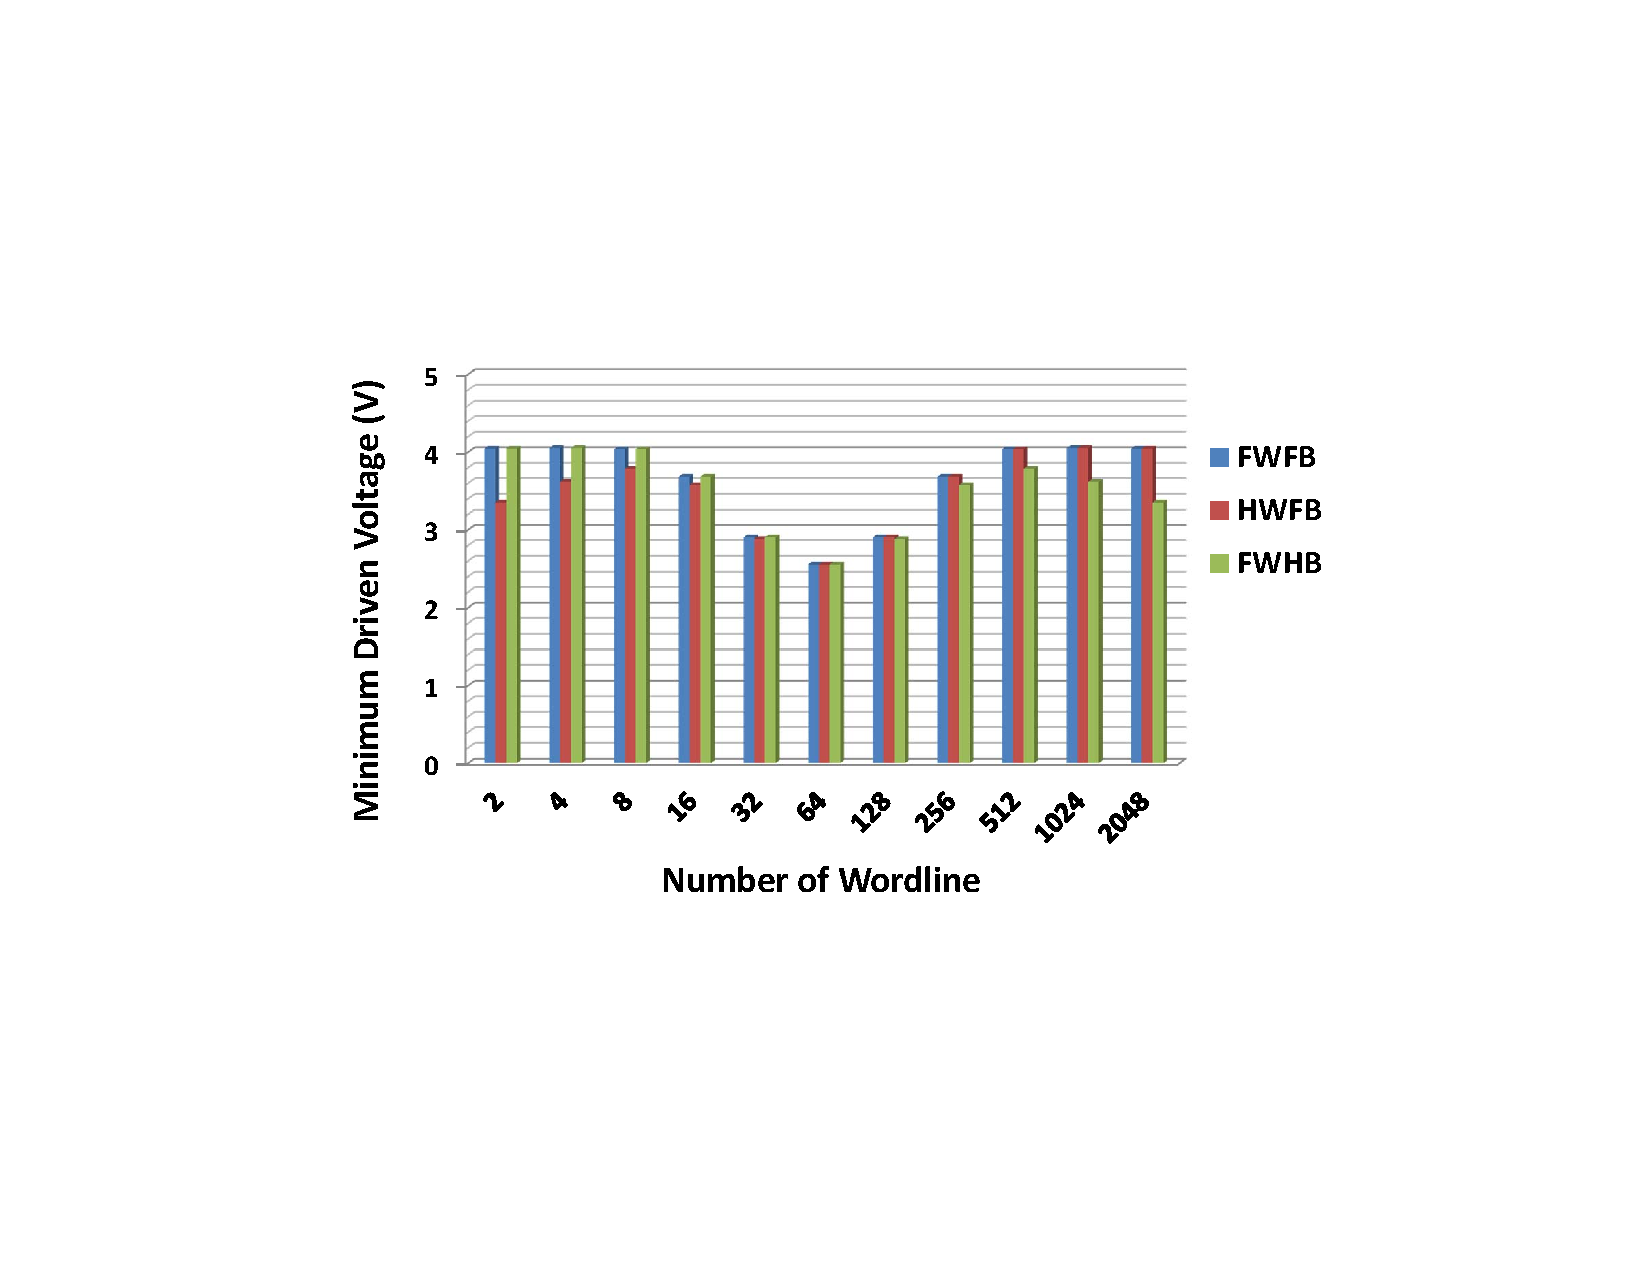
\includegraphics[width=0.45\textwidth]{./figures/shape_f.pdf}\\
  \caption{Required write voltages with different memory shapes (array capacity = 256Kbits, threshold voltage = 2V).}\label{fig:shape}
    \vspace{-15pt}
\end{figure}

However, boosting the driven voltage also introduces other potential
problems for the array. In particular, increasing the driven voltage also
increases the voltage applied at unselected cells. Therefore, a write
disturbance may occur when the voltage applied at an unselected cell
exceeds the threshold voltage for SET or RESET operation. Specifically,
the maximum voltage applied at unselect cells is exactly the same as half
of the driven voltage. Thus, only the array with driven voltage less than
4V are allowable.  Otherwise, the array is unreliable because it can not
avoid write failure and write disturbance at the same time. The unreliable
array sizes are denoted as red bars in Figure~\ref{fig:worst_v}. The array
size limitation provied by Figure~\ref{fig:worst_v} is a hard constraint
on array size, and all of the following energy and area tradeoffs should
be bounded by this constraint.


%Figure~\ref{fig:half} shows the maximum voltage applied at unselected
%cells with the minimum driven voltage, which is determined in
%Figure~\ref{fig:worst_v}. Since the threshold voltage of the ReRAM cell is
%2V, only array sizes with worst case unselected cell voltage less than 2V
%are allowable. Otherwise, the array is unreliable because it can not avoid
%write failure and write disturbance at the same time. Therefore,
%Figure~\ref{fig:half} provides a hard constraint on array size, and all of
%the following energy and area tradeoffs should be bounded by this
%constraint.

%\begin{figure}%[!t]
%\centering
%  % Requires \usepackage{graphicx}
%  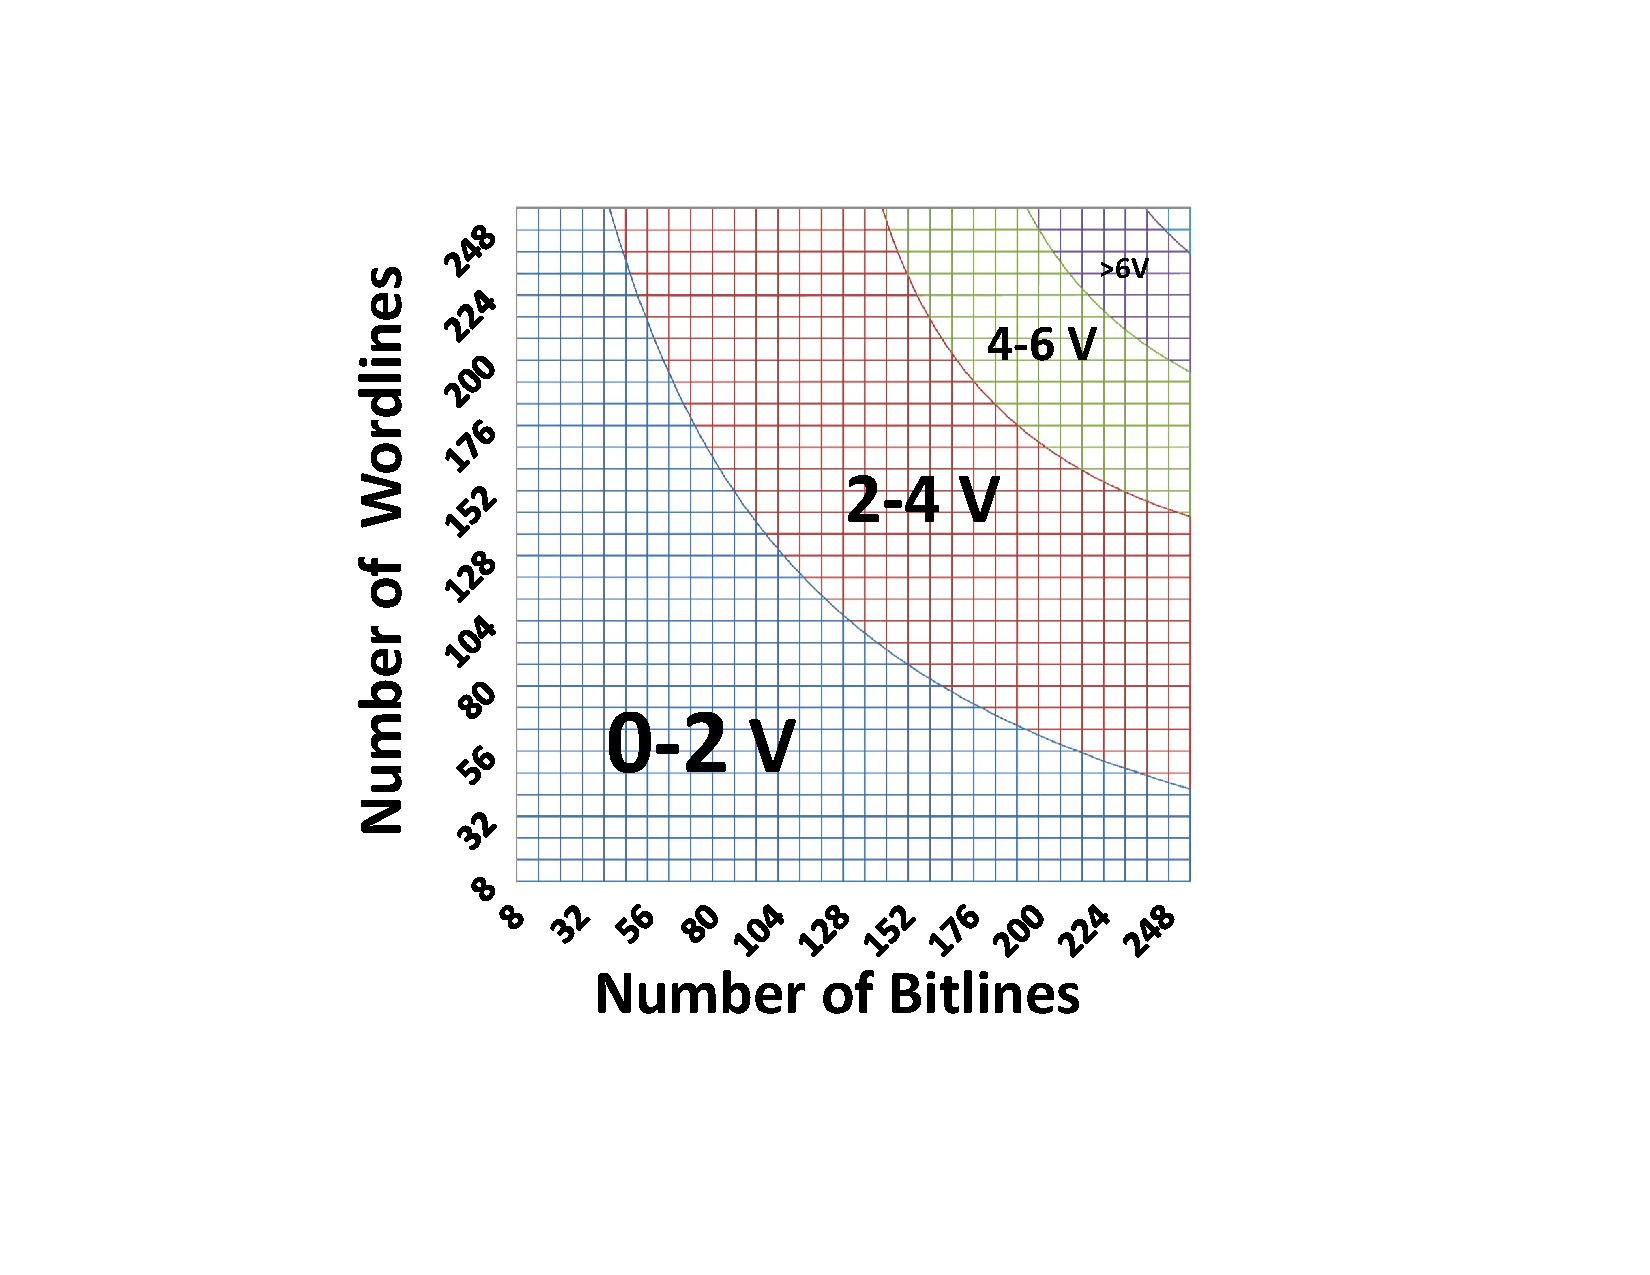
\includegraphics[width=0.28\textwidth]{./figures/Theoretical_bound_f.pdf}\\
%  \caption{The maximum voltage applied at unselected cells with the minimum driven voltage.}\label{fig:half}
%  \vspace{-10pt}
%\end{figure}


\vspace{6pt} \emph{Energy Consumption of Write Operation.} \vspace{6pt}

%The energy consumption of a write operation for a cross-point array can be calculated as:
%\begin{equation}
%E_{write} = E_{select} + E_{unselect} + E_{halfselect} + E_{line},
%\end{equation}
%where the $E_{select}$ is the energy consumed to change the state of the
%selected cell, the $E_{unselect}$ and $E_{halfselect}$ are the undesired
%energy wasted at the half selected and unselected cells. The energy
%consumed by the interconnect lines are represented by $E_{line}$.
%Figure~\ref{fig:energy} shows the decomposed energy consumption for the
%cross-point array. Note that, the $E_{line}$ and $E_{halfselect}$ take a
%large amount of the total energy consumption. Also, this part of energy
%wasted during the write operation takes greater part of the total energy
%for larger array sizes. For example, the undesired energy consumption for
%writing a $128{\times}128$ array is more than 1000 times larger than the
%$8{\times}8$ array. We also notice that, since the impact of sneak paths
%for floating schemes (FWHB and HWFB) is more serious, the energy consumed
%at unselected cells for floating schemes is larger than the half-biased
%scheme. Due to this reason, the total energy consumptions for FWHB and
%HWFB schemes are at least 10\% larger than that of HWHB scheme.
The energy consumption of a write operation includes: the energy consumed
to change the state of the selected cell (denoted as $E_{select}$), the
undesired energy wasted at the half selected cells ($E_{halfselect}$) and
unselected cells ($E_{unselect}$), as well as the energy consumed by the
interconnect lines ($E_{line}$). Notice that since the impact of sneak
paths for floating schemes (FWHB and HWFB) is more serious, the energy
consumed at unselected cells for floating schemes is larger than the
half-biased scheme. However, compared to the total energy consumption, the
energy consumed by unselected cells are negligible. Therefore, the total
energy consumptions for FWHB and HWFB schemes are almost the same as that
of HWHB scheme. In the following discussion, we focus on the HWHB scheme.
Figure~\ref{fig:energy}(a) shows the decomposed energy consumption for the
cross-point array. Note that, the $E_{line}$ and $E_{halfselect}$ take a
large amount of the total energy consumption. Also, this part of energy
wasted during the write operation takes greater part of the total energy
for larger array sizes. For example, the undesired energy consumption for
writing a $512{\times}512$ array is more than 15 times larger than that of
a $32{\times}32$ array.
\begin{figure}%[!t]
\centering
  % Requires \usepackage{graphicx}
  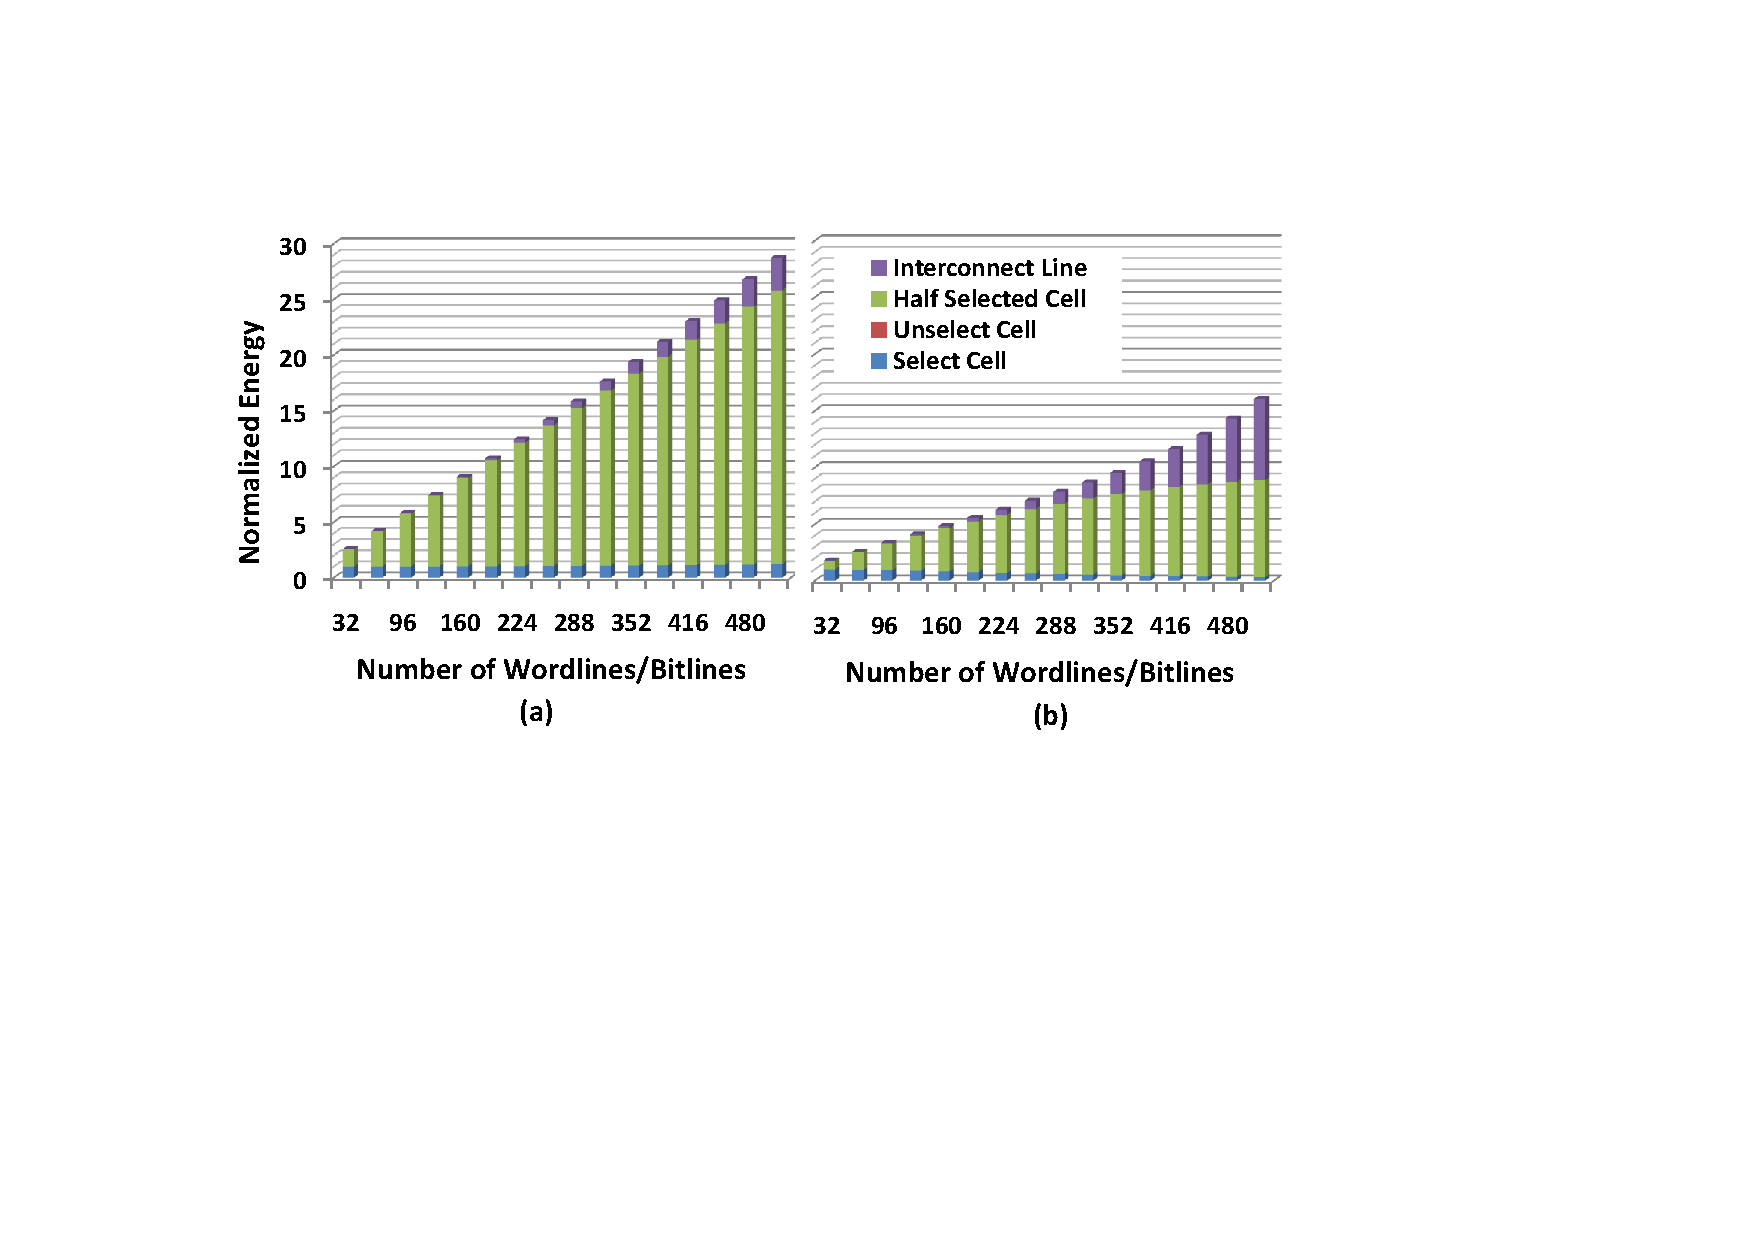
\includegraphics[width=0.5\textwidth]{./figures/energy_f_tall2.pdf}\\
  \caption{The normalized energy consumption with different array size. (a) Single-bit writing. (b) Multi-bit writing.}\label{fig:energy}
    \vspace{-10pt}
\end{figure}

\vspace{6pt} \emph{Write Current and Area Overhead of Write Operation.}
\vspace{6pt}

The write operation for a $M \times N$ array requires $M$ wordline voltage
drivers and $N$ bitline multiplexes. The drivers and multiplexes should be
sized such that they can provide the worst-case current of wordline
current and bitline current. The transistor sizing of the wordline/bitline
circuitry are achieved using HSPICE simulations. We further calculate the
area overhead for the drivers and multiplexes by referring to the CACTI
area model. Figure~\ref{fig:drive_i}(a) shows the maximum write current
with different ReRAM array sizes. Not surprisingly, the current
requirement increases as array size increases. Figure~\ref{fig:area_i}(a)
demonstrates the area overhead for the wordline and bitline circuitry. It
is indicated that wordline drivers occupies comparable or even larger area
than the memory cells, degrading the effective cell size significantly.
There are two possible reasons: (1) wordline drivers are usually
implemented as tri-gates and larger than bitline multiplexes that are
essentially pass transistors; (2) wordline drivers have to provide more
than one set of write current in multi-bits write operation, as discussed
in the following section.

%\begin{figure}%[!t]
%\centering
%  % Requires \usepackage{graphicx}
%  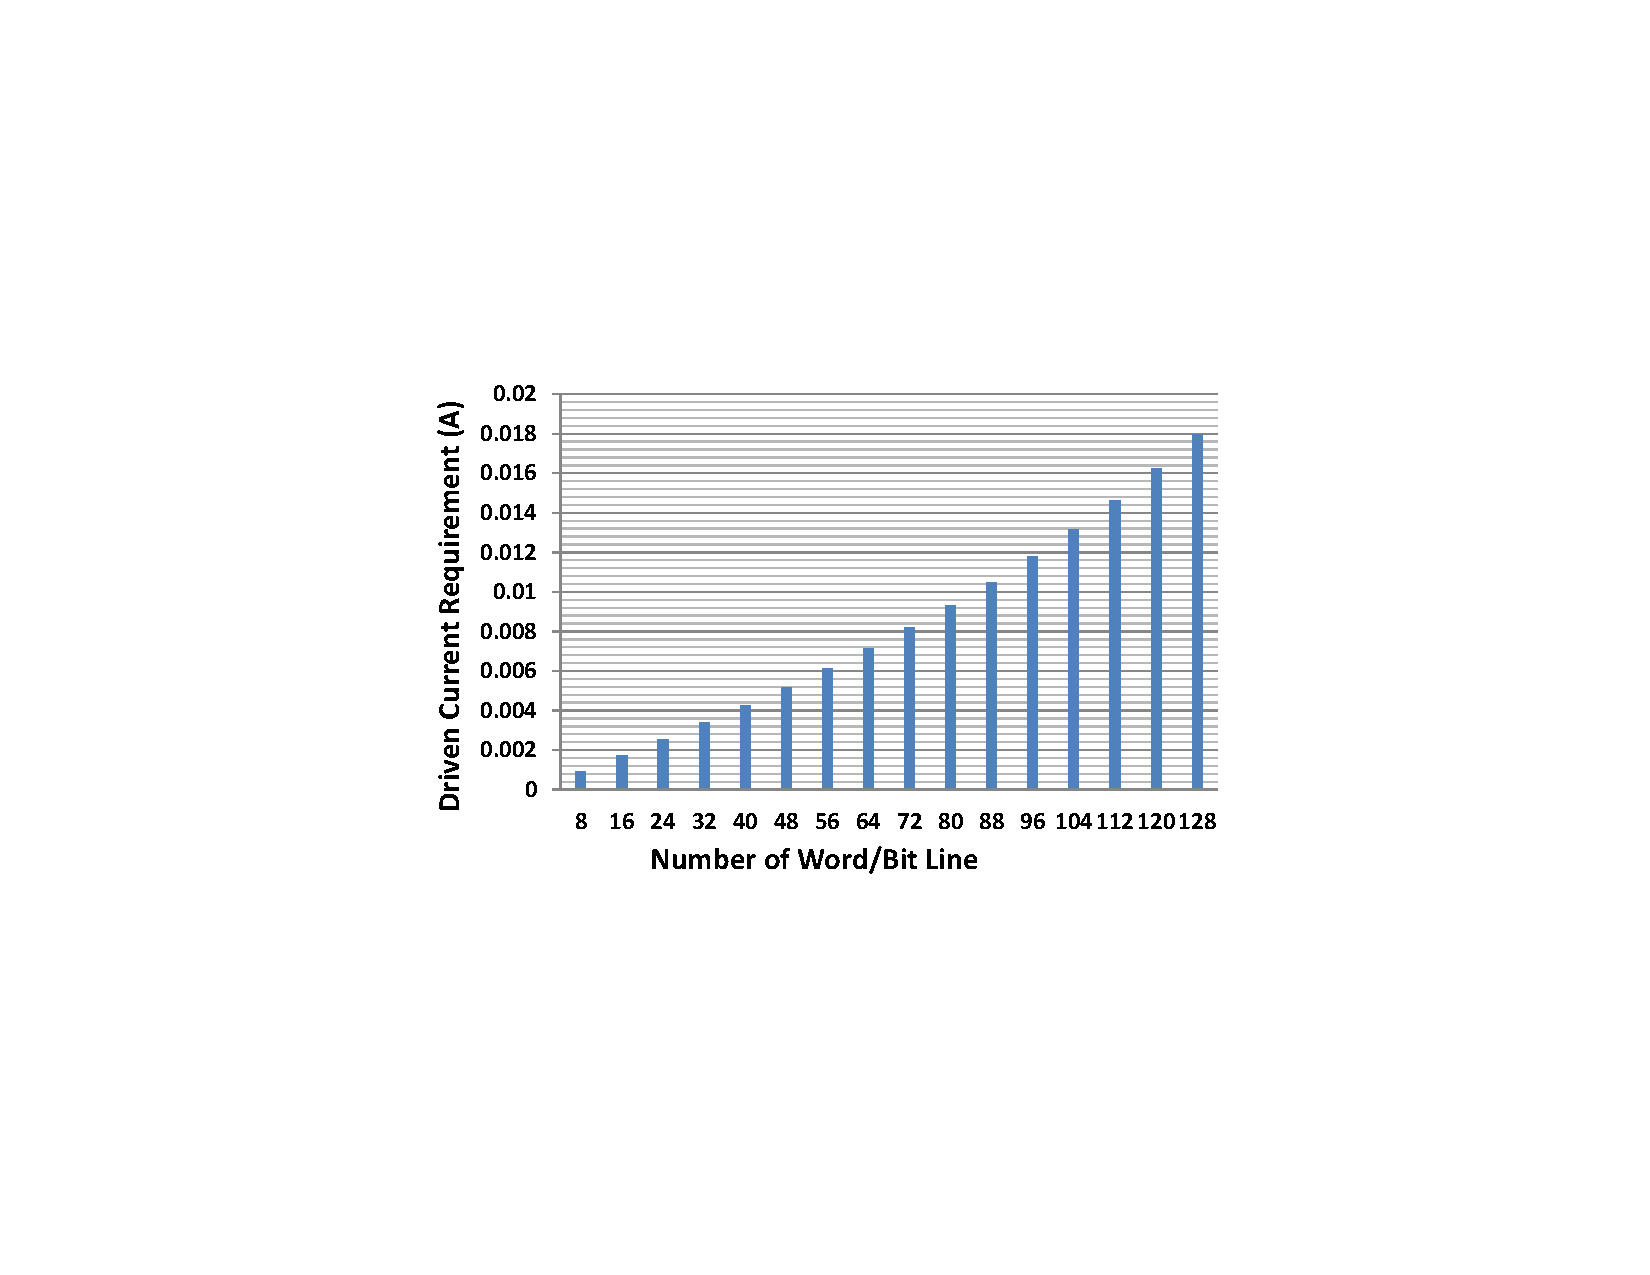
\includegraphics[width=0.4\textwidth]{./figures/w_current2.pdf}\\
%  \caption{The }\label{fig:w_current}
%\end{figure}
\begin{figure}%[!t]
\centering
  % Requires \usepackage{graphicx}
  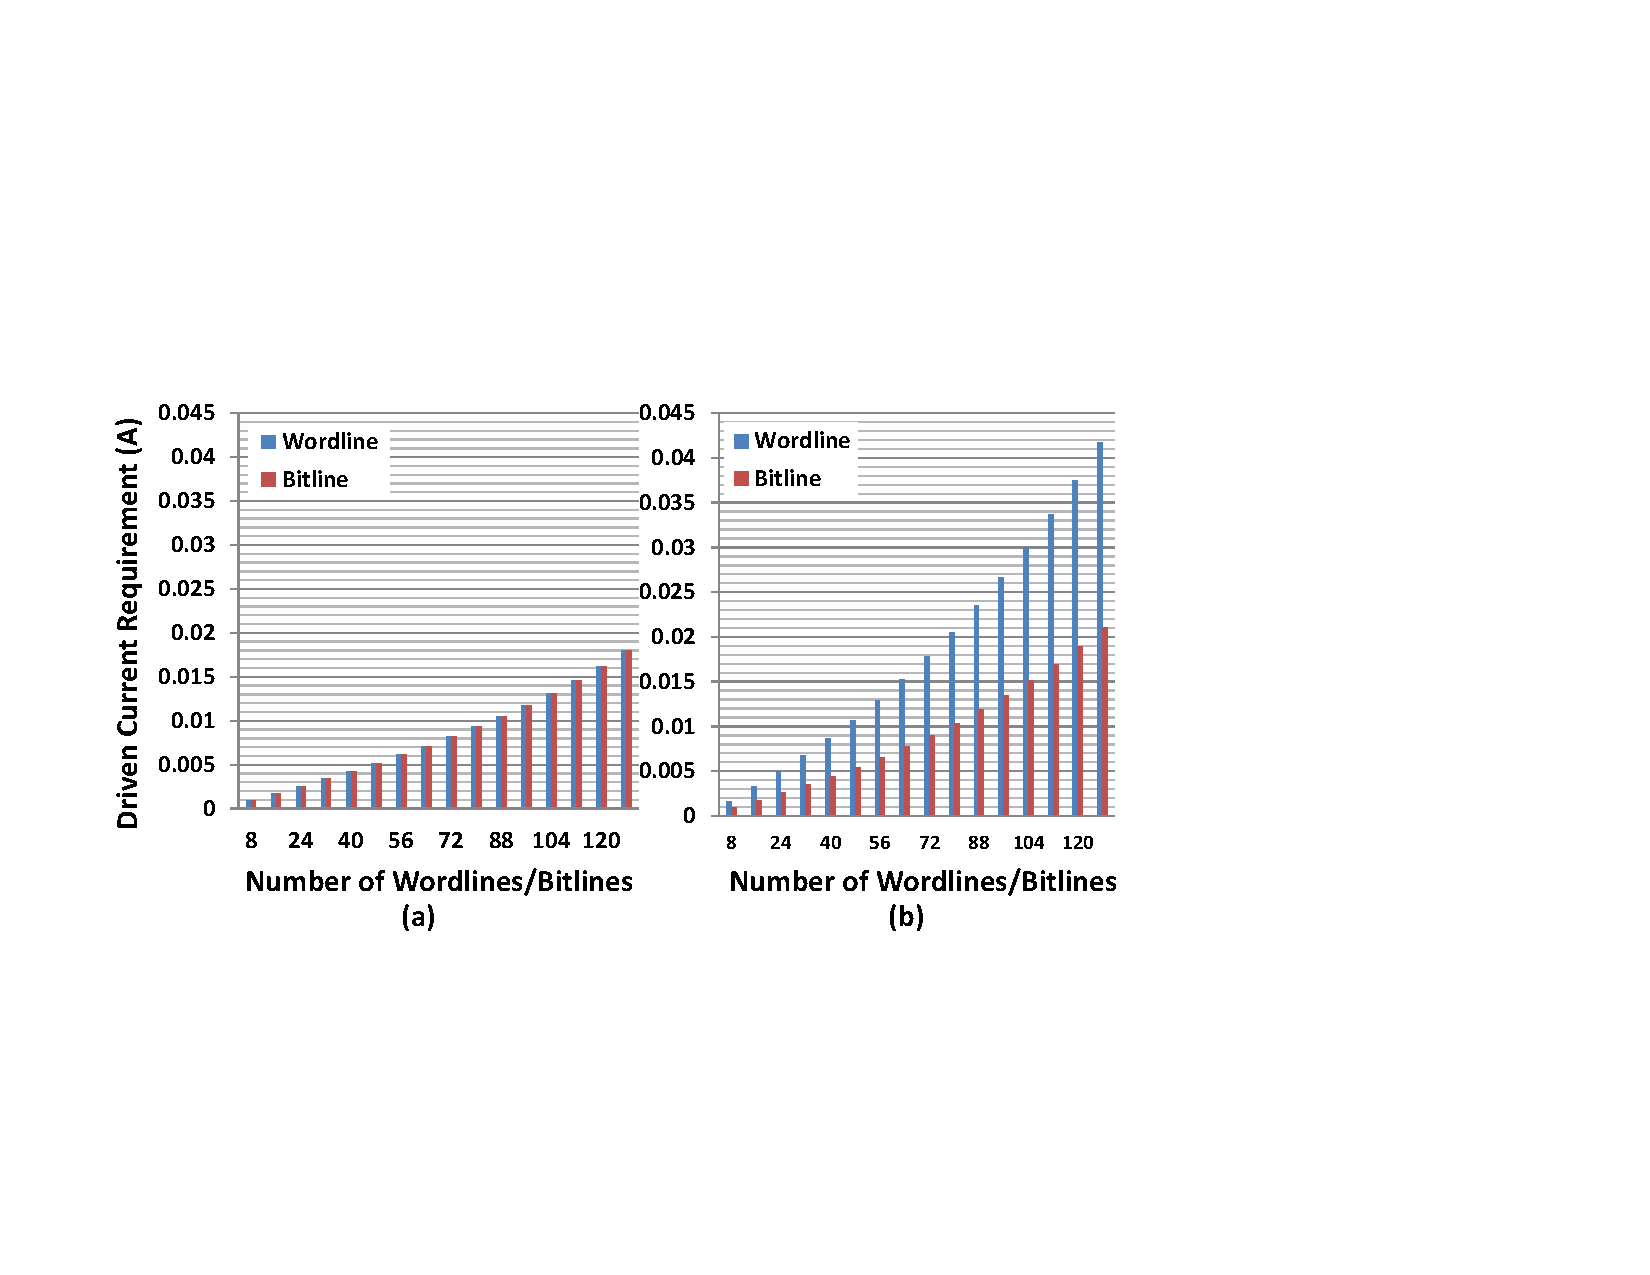
\includegraphics[width=0.5\textwidth]{./figures/drive_i_f.pdf}\\
  \caption{The requirements for wordline and bitline driven currents. (a) One bit per write. (b) One wordline per write.}\label{fig:drive_i}
\end{figure}



\begin{figure}%[!t]
\centering
  % Requires \usepackage{graphicx}
  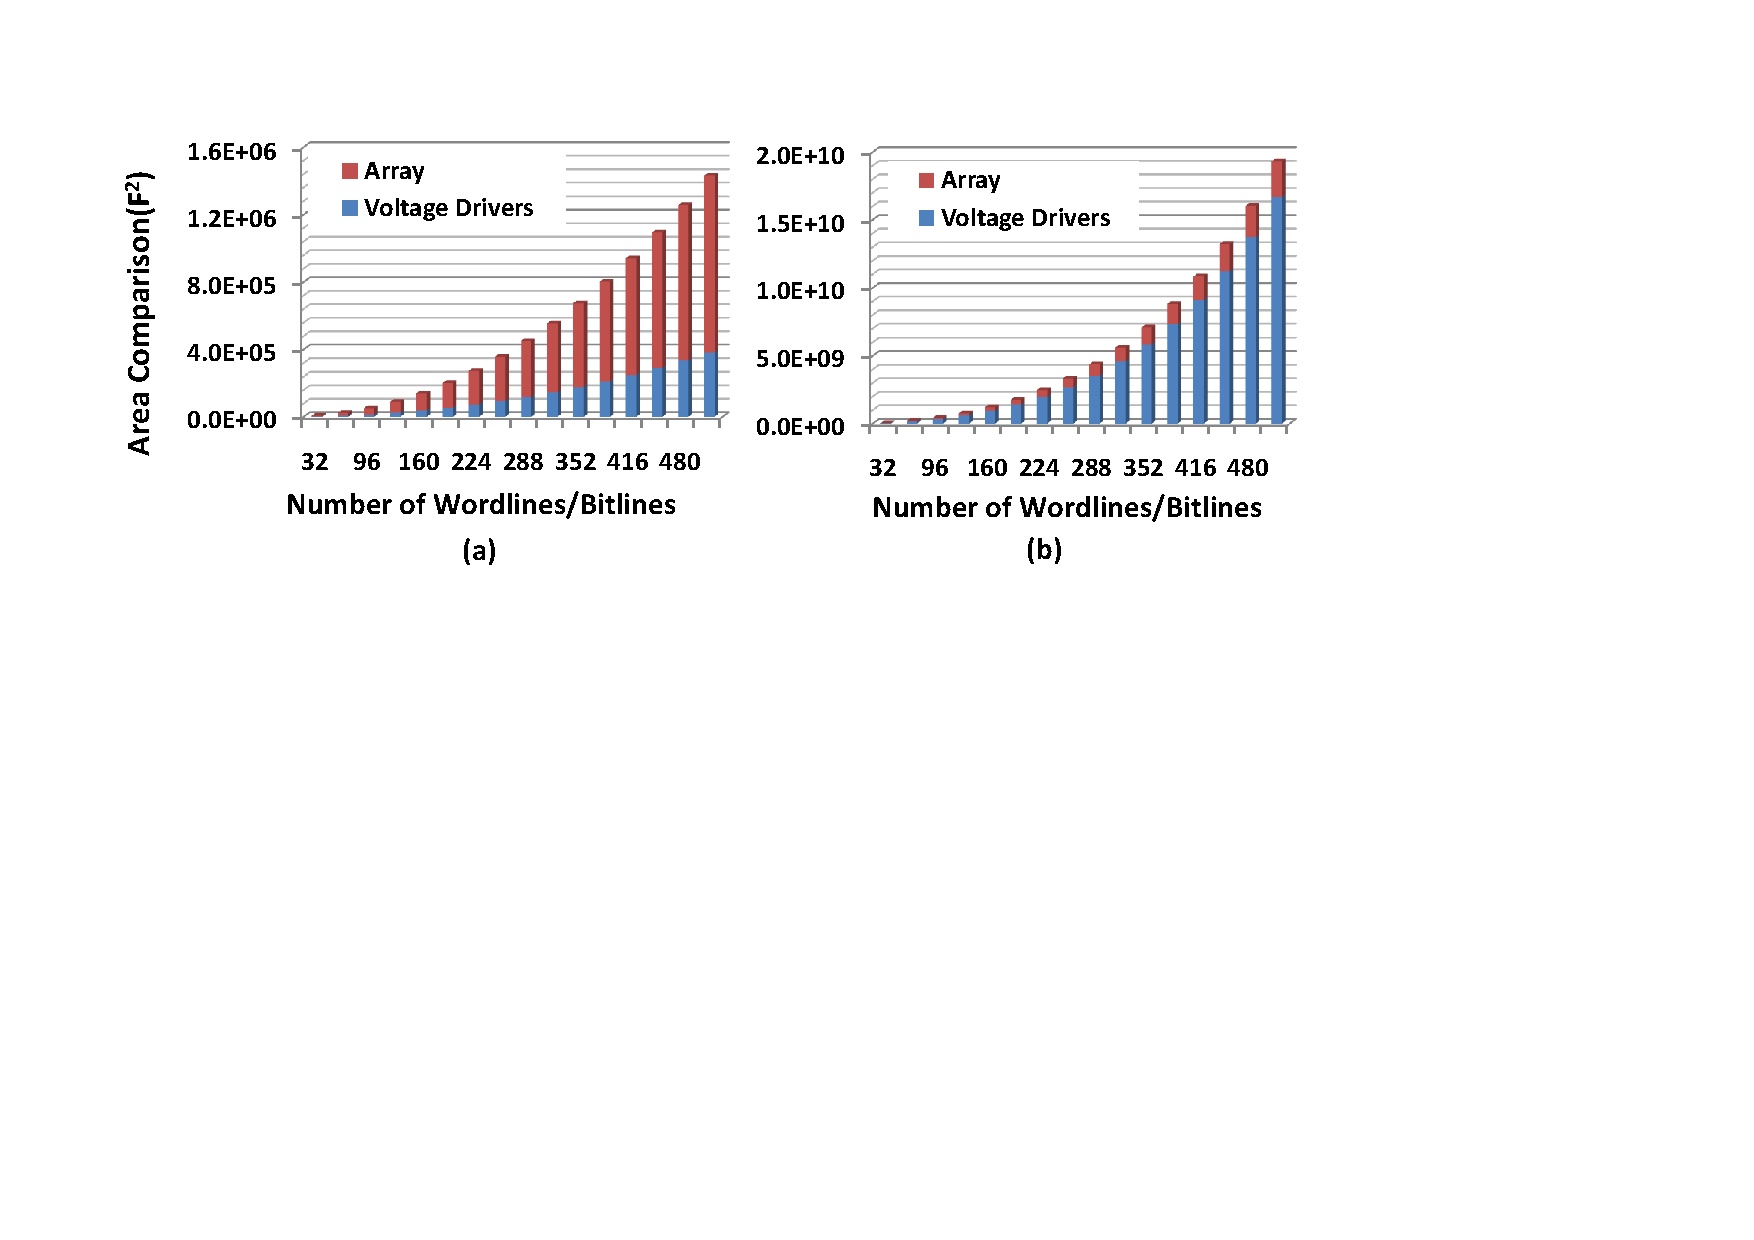
\includegraphics[width=0.5\textwidth]{./figures/area_comp_f.pdf}\\
  \caption{Area overhead comparison. (a) One bit per write (B) One wordline per write.}\label{fig:area_i}
\vspace{-10pt}
\end{figure}

\vspace{6pt} \emph{Discussion on Multi-Bits Write Operation.} \vspace{6pt}

So far, we have only discussed the write operation with one bit per
access. In this section, we consider the difference between single-bit per
access and multi-bit per access write operations.

First of all, we evaluate the energy consumption of the write operation
that program one wordline at the same time. In order to fairly compare the
energy consumption, we compare the energy-per-bit instead of the total
energy. For example, in order to write a wordline with size of 512, the
energy-per-bit can be calculated as: $E_{ave}=E_{total}/512$.
Figure~\ref{fig:energy}(b) shows the energy-per-bit of the multi-bit write
operation. Compared with the single-bit write operation, as shown in
Figure~\ref{fig:energy}(a),the results show that for large cross point
array sizes, the multi-bit write operation is much more energy efficient.
This is because the energy wasted at the unselected and half-selected
cells are amortized by multiple bits and the average energy for one bit is
therefore reduced. However, although the multi-bit write operation has the
advantage of lower energy consumption, the maximum current requirement for
each wordline also increases. As demonstrated in
Figure~\ref{fig:drive_i}(b), although the maximum driven current for each
bitline is almost the same as when writing one bit, the driving current
requirement for each word line in multi-bit write scheme is $>10$ times
larger than that of single-bit write scheme. Since the area of the voltage
driver increases proportionally with its driving current, the area
overhead for multi-bit writing is much larger than that of single-bit
write scheme.


%\begin{figure}%[!t]
%\centering
%  % Requires \usepackage{graphicx}
%  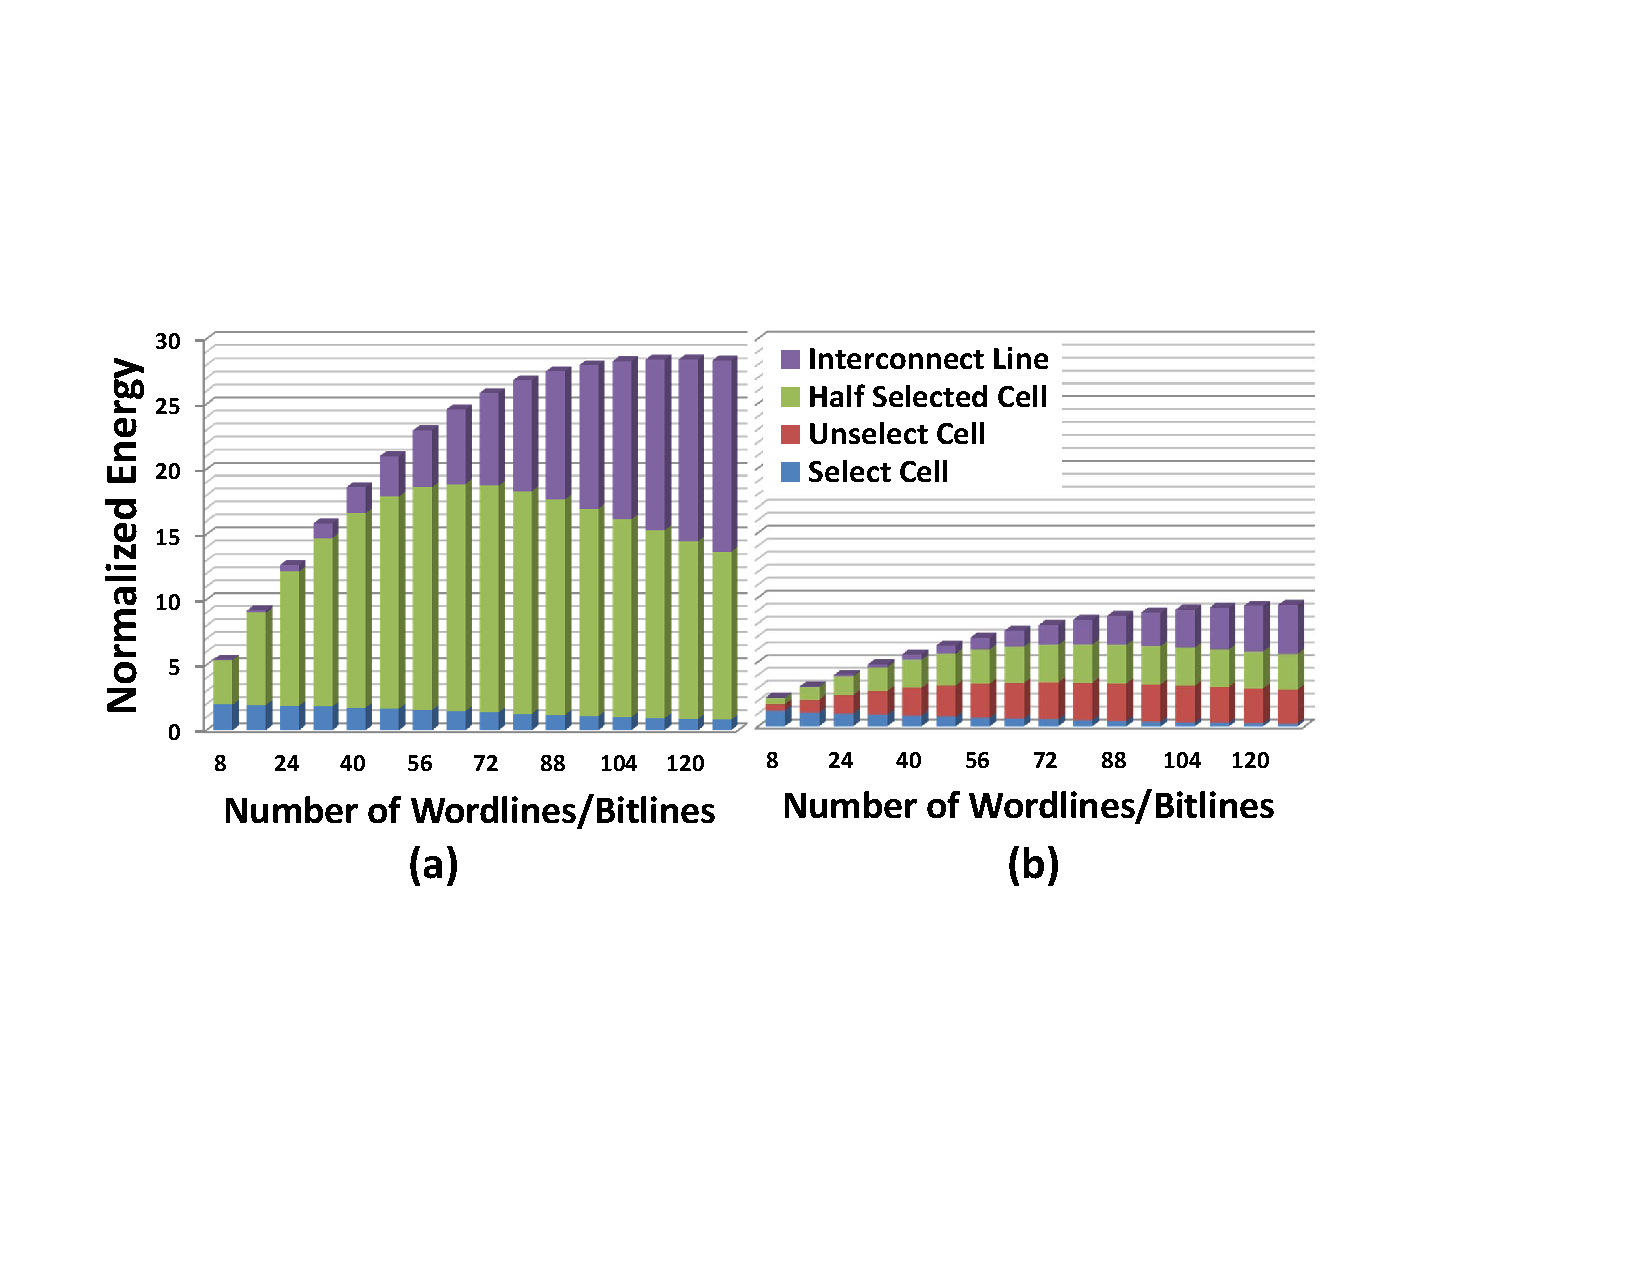
\includegraphics[width=0.5\textwidth]{./figures/multi_energy_f.pdf}\\
%  \caption{The normalized energy consumption per bit for multi-bits write operation. (a): HWHB and  FWHB schemes; (b): HWFB scheme. }\label{fig:multi_energy}
%    \vspace{-10pt}
%\end{figure}

In addition to the extra area overhead, writing multiple bits at one time
also worsens the voltage drop along the wordline. As shown in Figure~9(a),
in order to write a wordline per writing, the reliable array size reduces
to $352 \times 352$. This is because the current passing through the
interconnect wires in multi-bit write scheme is much larger than that of
single-bit write scheme, causing more severe voltage drop on the wire
resistance. Figure~9(b) shows that for a $512\times 512$ cross-point
array, the worst-case voltage drop increases and eventually become
unreliable as we increase the number of bits per write operation. The
maximum of bits that can be accessed simultaneously while maintaining
reliable write operation is about 130.

%Therefore, as shown in Figure~\ref{fig:reliable_region},
%Therefore the simulation results show that the reliable size of the
%cross-point array will be further reduced. The maximum array size reduces
%from $116{\times}116$ to $100{\times}100$ for HWFB and HWFB schemes.
%For the energy consumption point of view, the one wordline write operation is more efficient.
\begin{figure}%[!t]
\centering\label{fig:multiV}
  % Requires \usepackage{graphicx}
  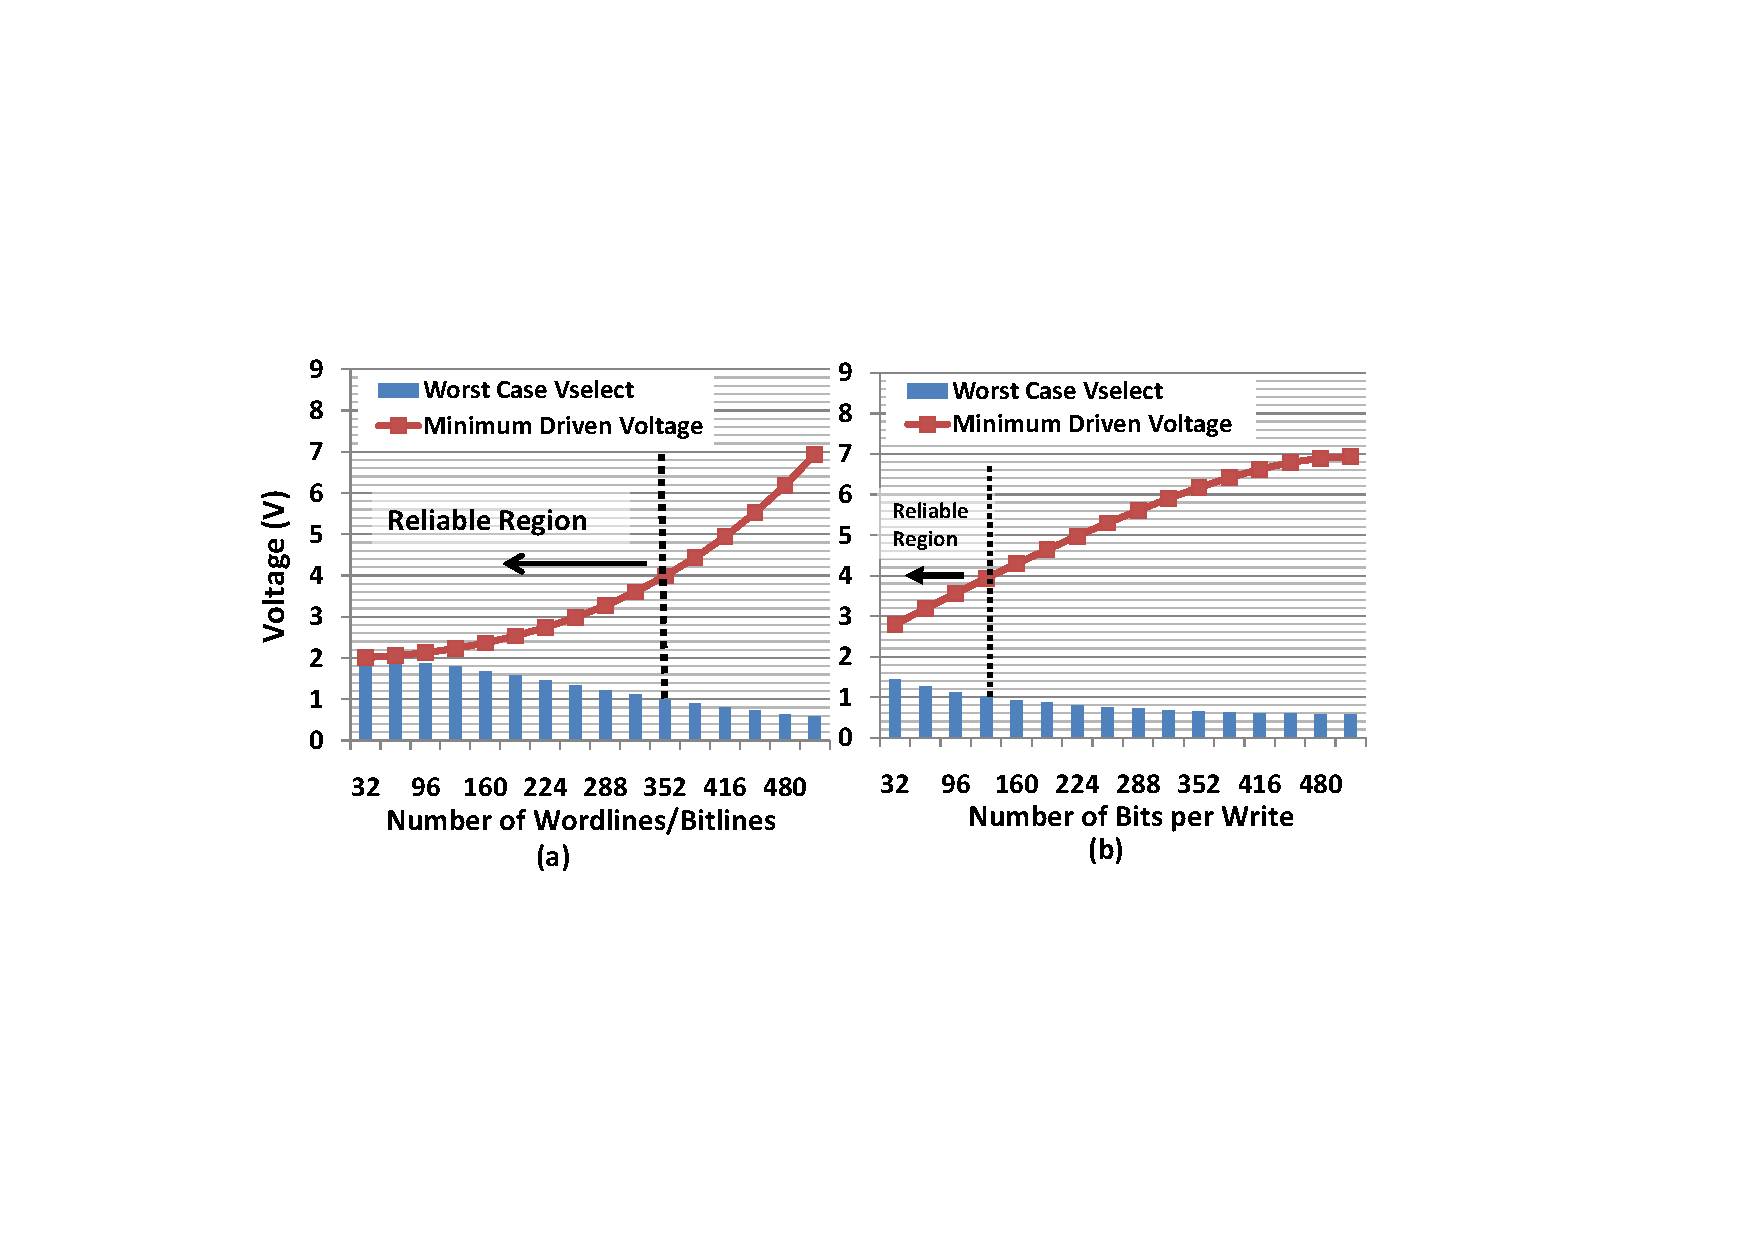
\includegraphics[width=0.5\textwidth]{./figures/multi_V.pdf}\\
  \caption{Worst case voltage and write voltage requirements for multi-bit writing. (a) Writing all the bits in a wordline at the same time (x-axis denote the different array sizes). (b) Writing various bits per operation in a 512$\times$512 array.}\label{fig:reliable_region}
    \vspace{-10pt}
\end{figure}
\subsection{Read Operation}
In this section we applied the similar sensing scheme as
\cite{crossbar_TED_2010} and \cite{crossbar_NANO08_Flocke}. In order to
read cell $R_{i,j}$, the $i^{th}$ wordline is biased at $V_{READ}$ and all
of the other wordlines and bitlines are grounded. Then the state of the
selected cell is read out by measuring the voltage across $R_s$. The
energy consumption for read operation can be analyzed by the same way as
that of the write operation. Since the read voltage is much smaller than
write voltage, the read energy is expected at least one order magnitude
smaller than write operation. Considerable sensing margin is achieved by
implementing a current-to-voltage converter and sensing the voltage signal
using traditional or emerging sense amplifier design. The input resistance
of the current-to-voltage converter is extracted from HSPICE simulation
results. Read sensing margin is defined as $\Delta V = \Delta I \times
R_{converter}$ where $R_{converter}$ is input resistance of the converter.
The read reliability is determined by the voltage swing for reading HRS
and LRS cells. In order to improve the reliability of the read operation,
a two-step sensing scheme can be applied~\cite{memristor:Cong}, which
senses the current of an unselected cell first, then the overall current
is sensed, and after that the current difference is converted to the
output voltage. More detailed results will be shown in
Section~\ref{sec:scale}.

%Additionally, since the read voltage/current is much lower than the write voltage/current, we believe that the voltage drivers can always provide enough current for the read operation if they meet the current requirement for write operation. Therefore, we can conclude that the area overhead of voltage drivers is determined by the write current. However, the reliability of read operation is different from the write operation. Figure~\ref{fig:sense_margin_basic} (a) shows the voltage swing with different array sizes. Specifically, larger cross-point array have more sneak paths, making the output voltage very sensitive to the data pattern of unselected cell. Therefore, the sense margin decreases with the increase of array size.  The voltage swing of this two-step sensing scheme is shown in Figure~\ref{fig:sense_margin_basic} (b). By using this two-step sensing schemes, the voltage swing for a given array size and non-linearity coefficient is doubled.


%\begin{figure}%[!t]
%\centering
%  % Requires \usepackage{graphicx}
%  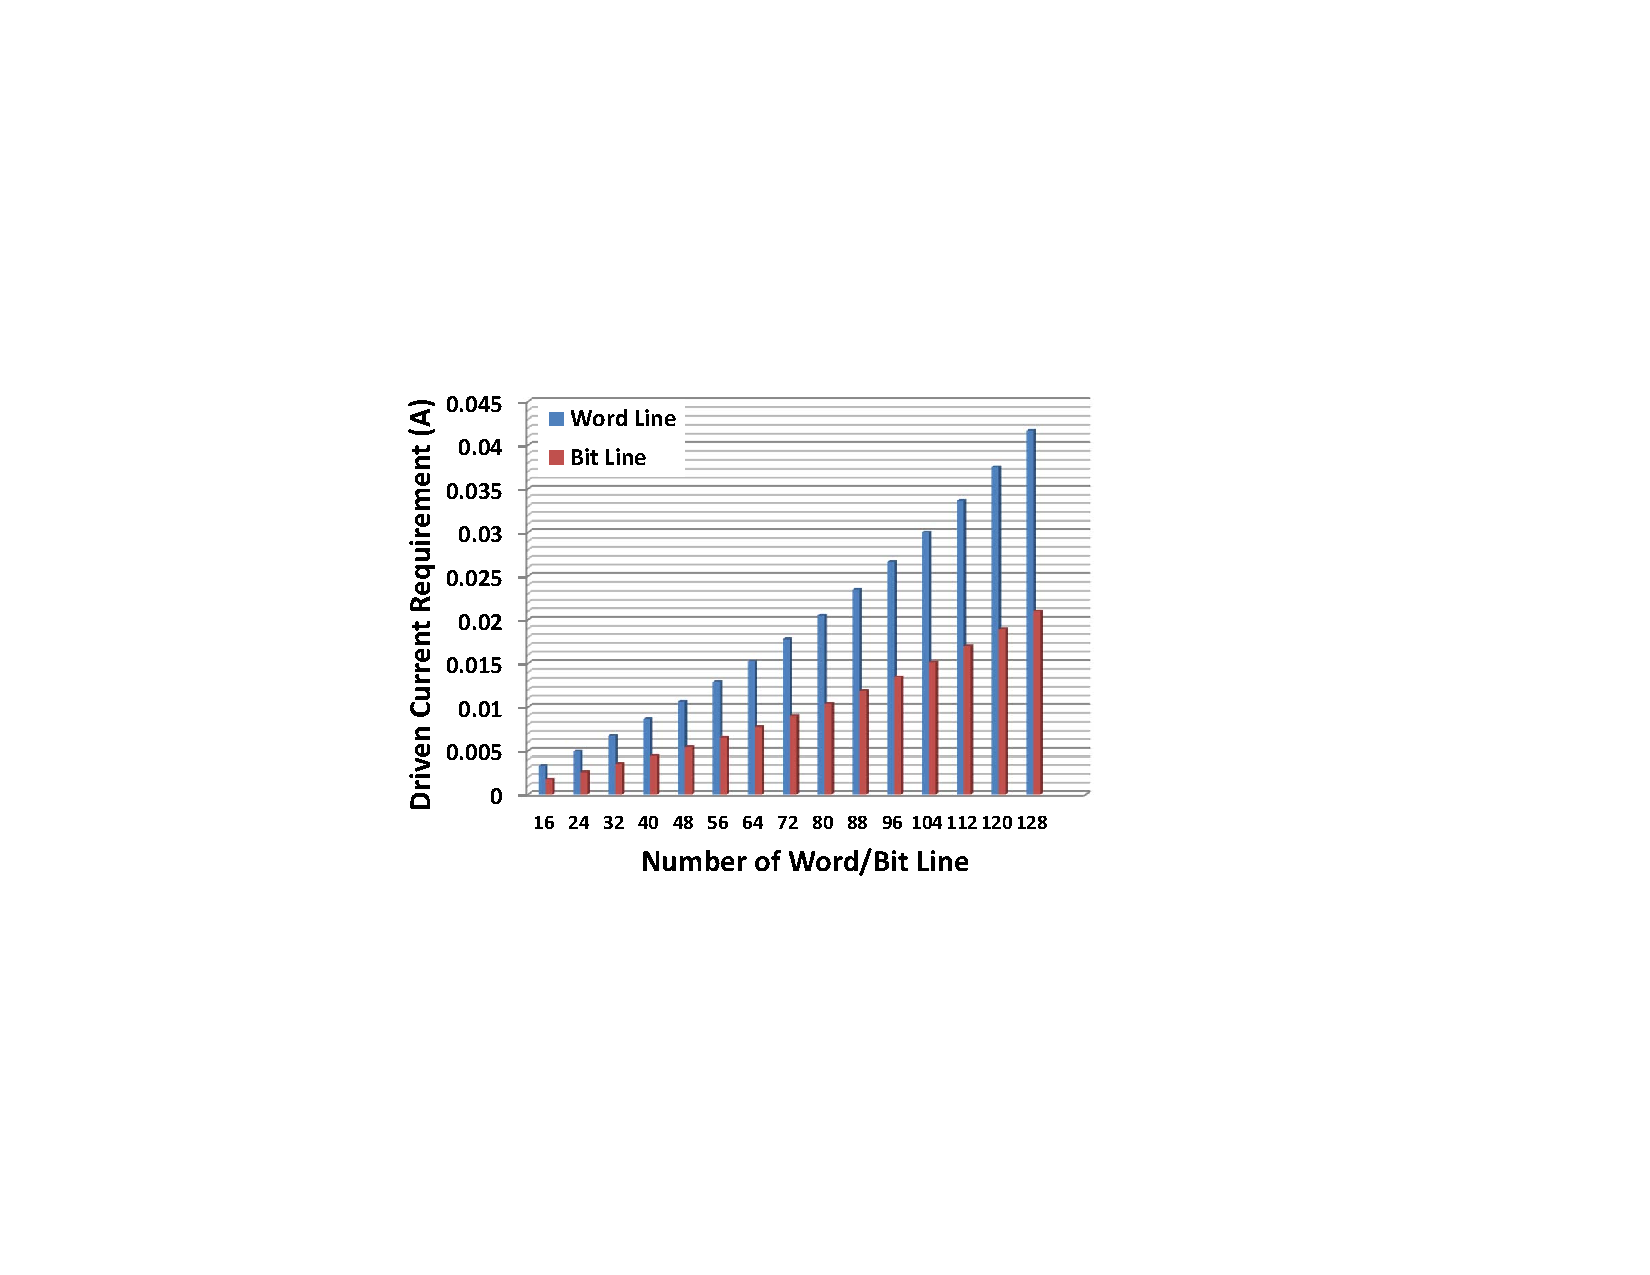
\includegraphics[width=0.4\textwidth]{./figures/multi_I2.pdf}\\
%  \caption{The }\label{fig:multi_I}
%\end{figure}


%\subsection{Read Operation}
%In this section we applied the similar sensing scheme as
%\cite{crossbar_TED_2010} and \cite{crossbar_NANO08_Flocke}. In order to
%read cell $R_{i,j}$, the $i^{th}$ wordline is biased at $V_{READ}$ and all
%of the other wordlines and bitlines are grounded. Then the state of the
%selected cell is read out by measuring the voltage across $R_s$. The
%energy consumption for read operation can be analyzed by the same way as
%that of the write operation. Since the read voltage is much smaller than
%write voltage, the read energy is expected at least one order smaller than
%write operation. Additionally, since the read voltage/current is much
%lower than the write, we believe that the voltage drivers can always
%provide enough current for the read operation if they meet the current
%requirement for write operation. Therefore, we can conclude that the area
%overhead of voltage drivers is determined by the write current. However,
%the reliability of read operation is different from the write operation.
%The read reliability is determined by the voltage swing for reading HRS
%and LRS cells. Figure~\ref{fig:sense_margin} (a) shows the voltage swing
%with different array sizes and $K_r$ values. Large array sizes and large
%non-linearity are harmful to the voltage swing: on the one hand, a larger
%array has more sneak paths, making the output voltage very sensitive to
%the data pattern of unselected cells; on the other hand, the non-linearity
%increases the resistance of LRS and therefore the resistance difference
%between HRS and LRS cells is reduced. In order to improve the reliability
%of the read operation, a two-step sensing scheme can be applied, which
%senses the current of an unselected cell first, then the overall current
%is sensed, and after that the current difference is converted to the
%output voltage. The voltage swing of this two-step sensing scheme is shown
%in Figure~\ref{fig:sense_margin} (b). By using this two-step sensing
%schemes, the voltage swing for a given array size and non-linearity
%coefficient is doubled.
%
%%\begin{figure}%[!t]
%%\centering
%%  % Requires \usepackage{graphicx}
%%  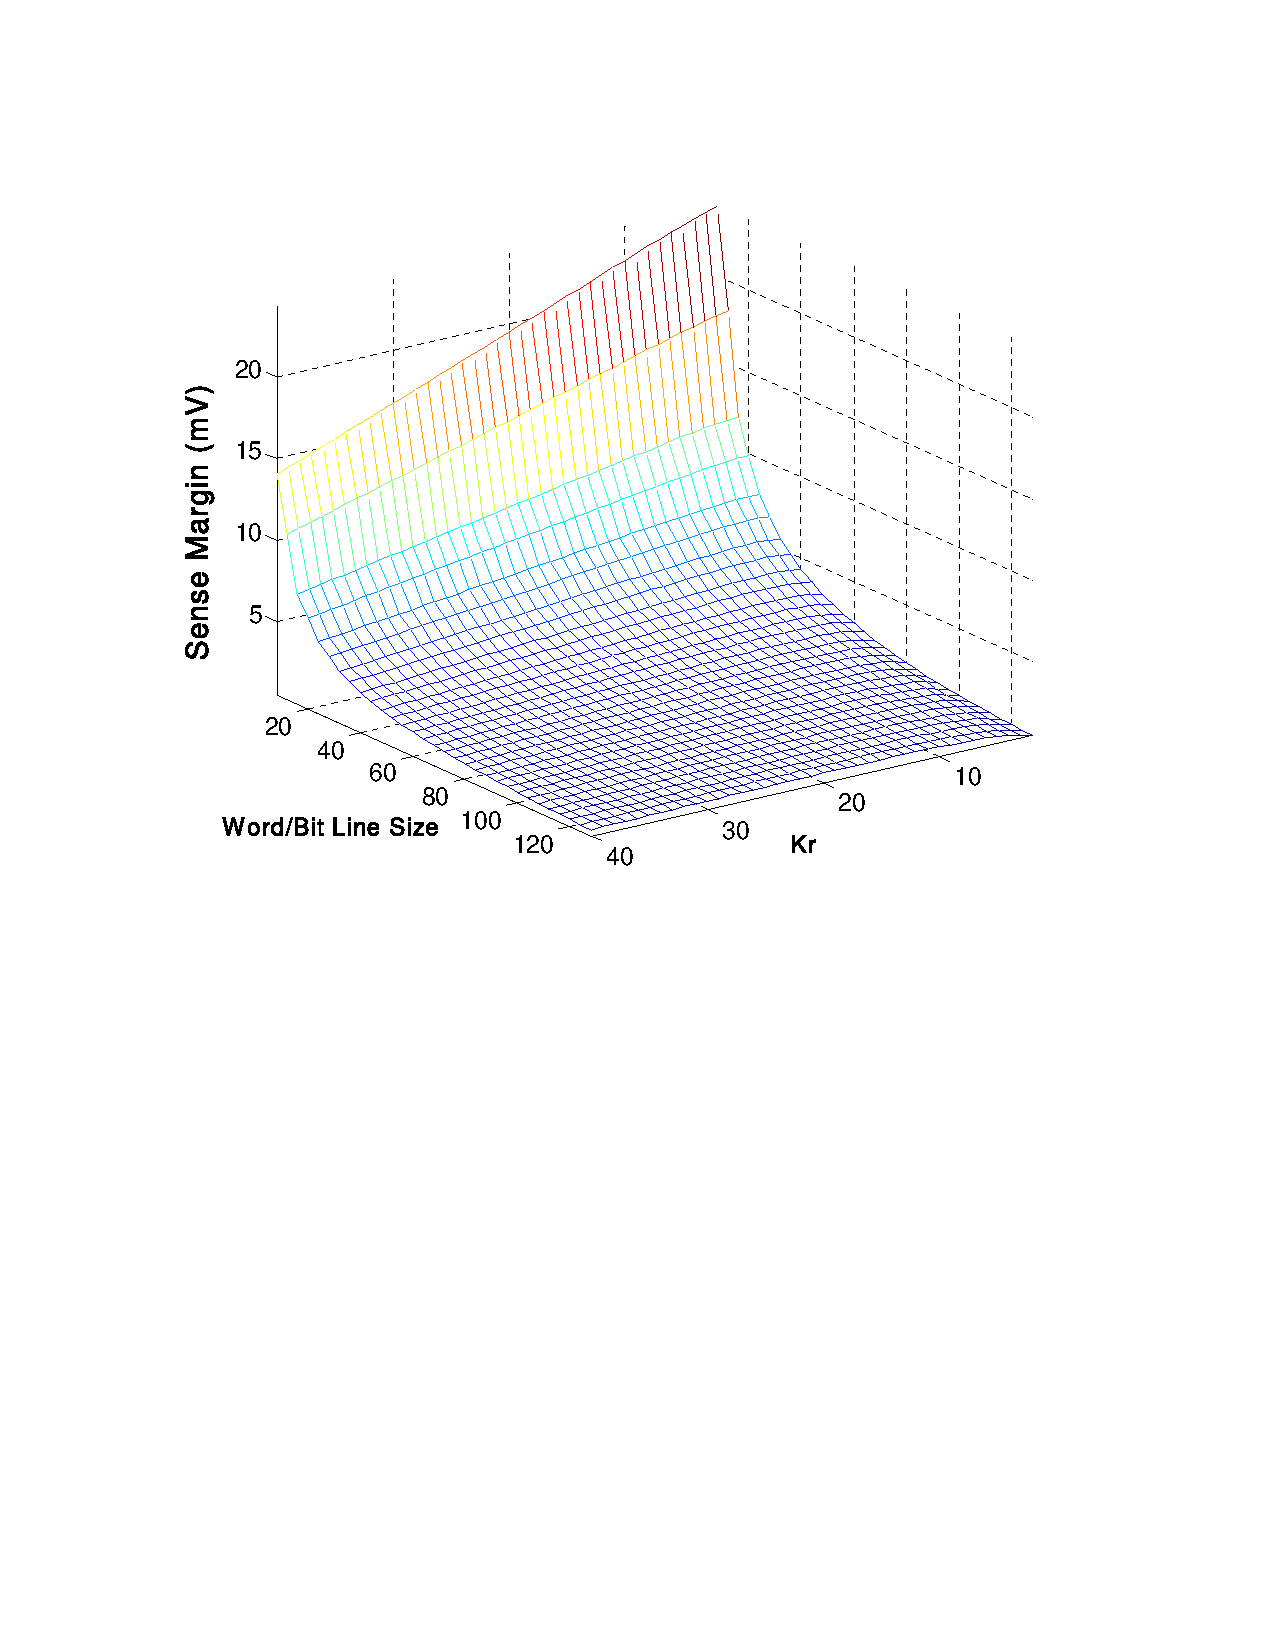
\includegraphics[width=0.45\textwidth]{./figures/margin.pdf}
%%  \caption{The}\label{fig:margin}
%%\end{figure}
%%
%%\begin{figure}%[!t]
%%\centering
%%  % Requires \usepackage{graphicx}
%%  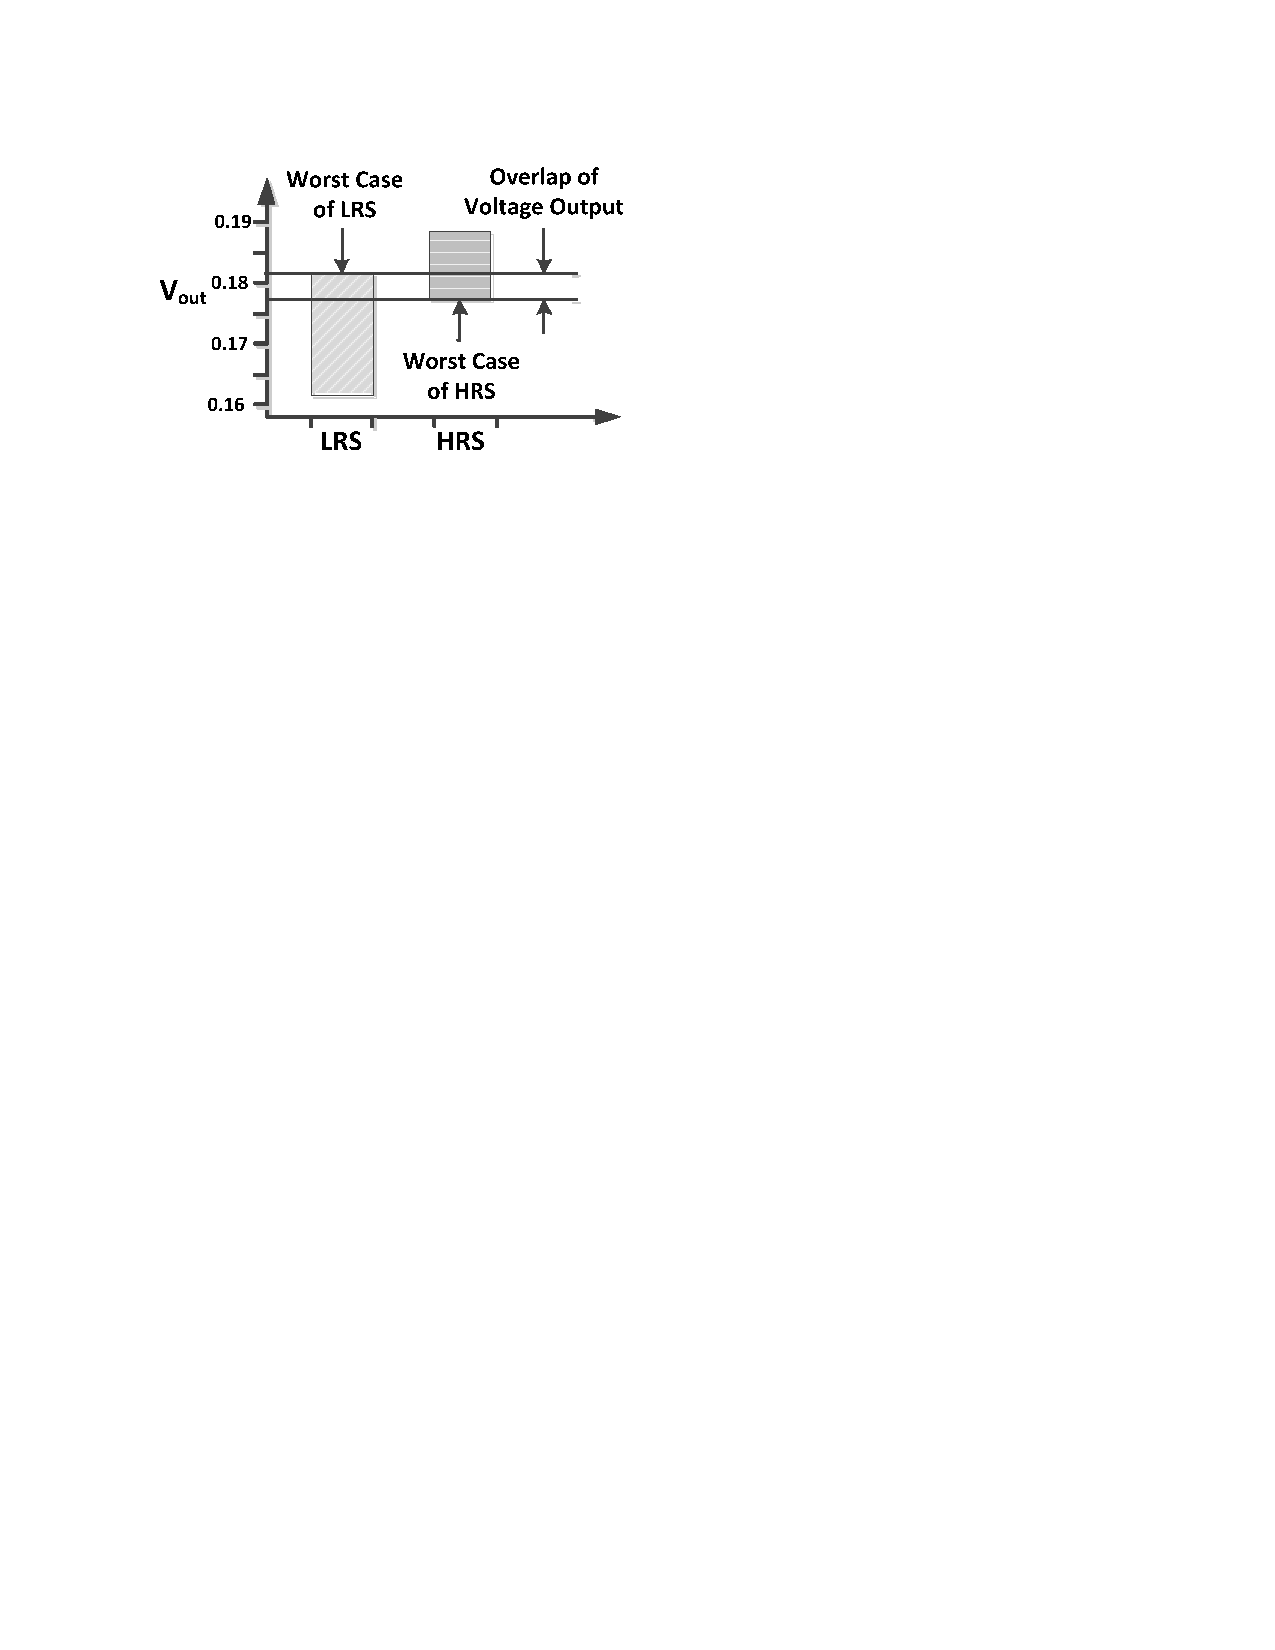
\includegraphics[width=0.4\textwidth]{./figures/overlap.pdf}\\
%%  \caption{The}\label{fig:overlap}
%%\end{figure}
%
%%
%%\begin{figure}%[!t]
%%\centering
%%  % Requires \usepackage{graphicx}
%%  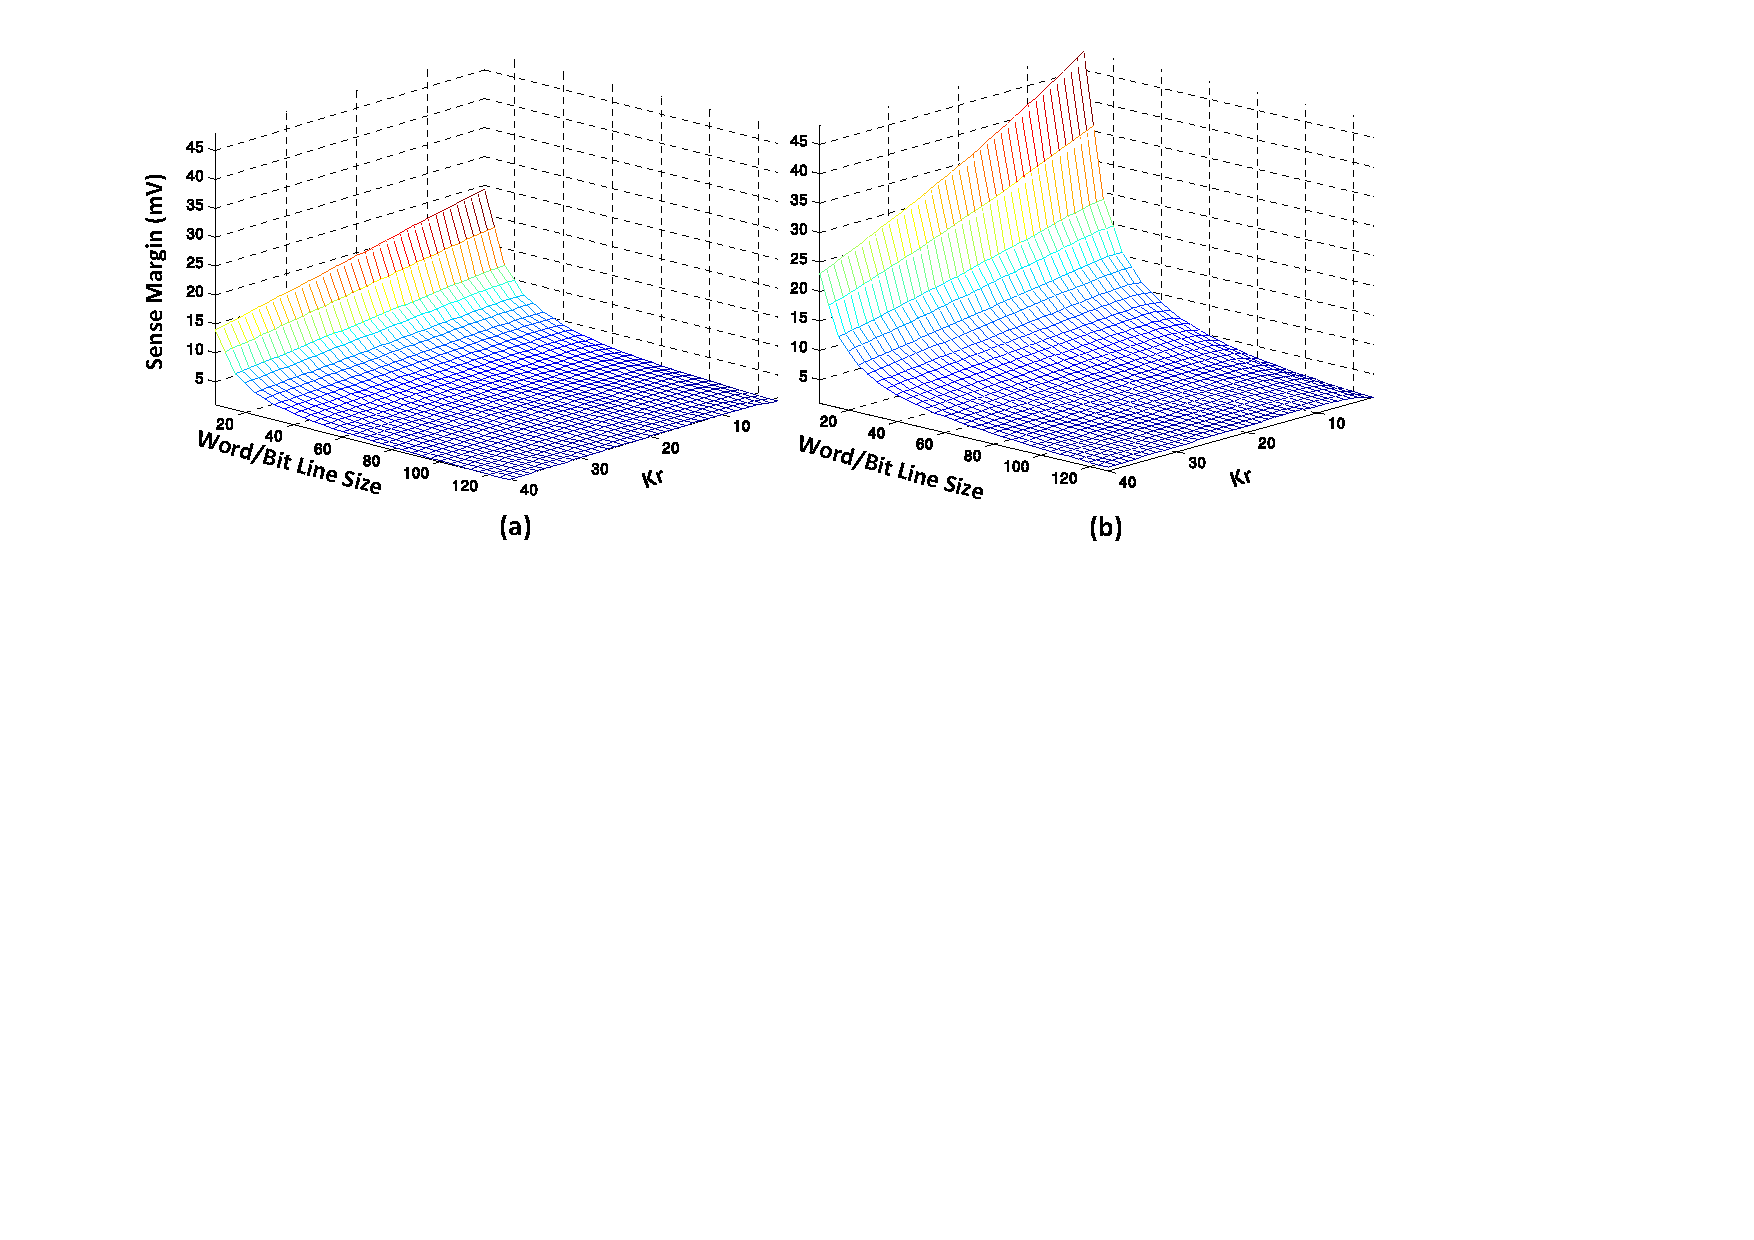
\includegraphics[width=0.5\textwidth]{./figures/sense_margin21}\\
%%  \caption{The}\label{fig:sense_margin}
%%\end{figure}
%
%\begin{figure}[!b]
%\centering
%  % Requires \usepackage{graphicx}
%  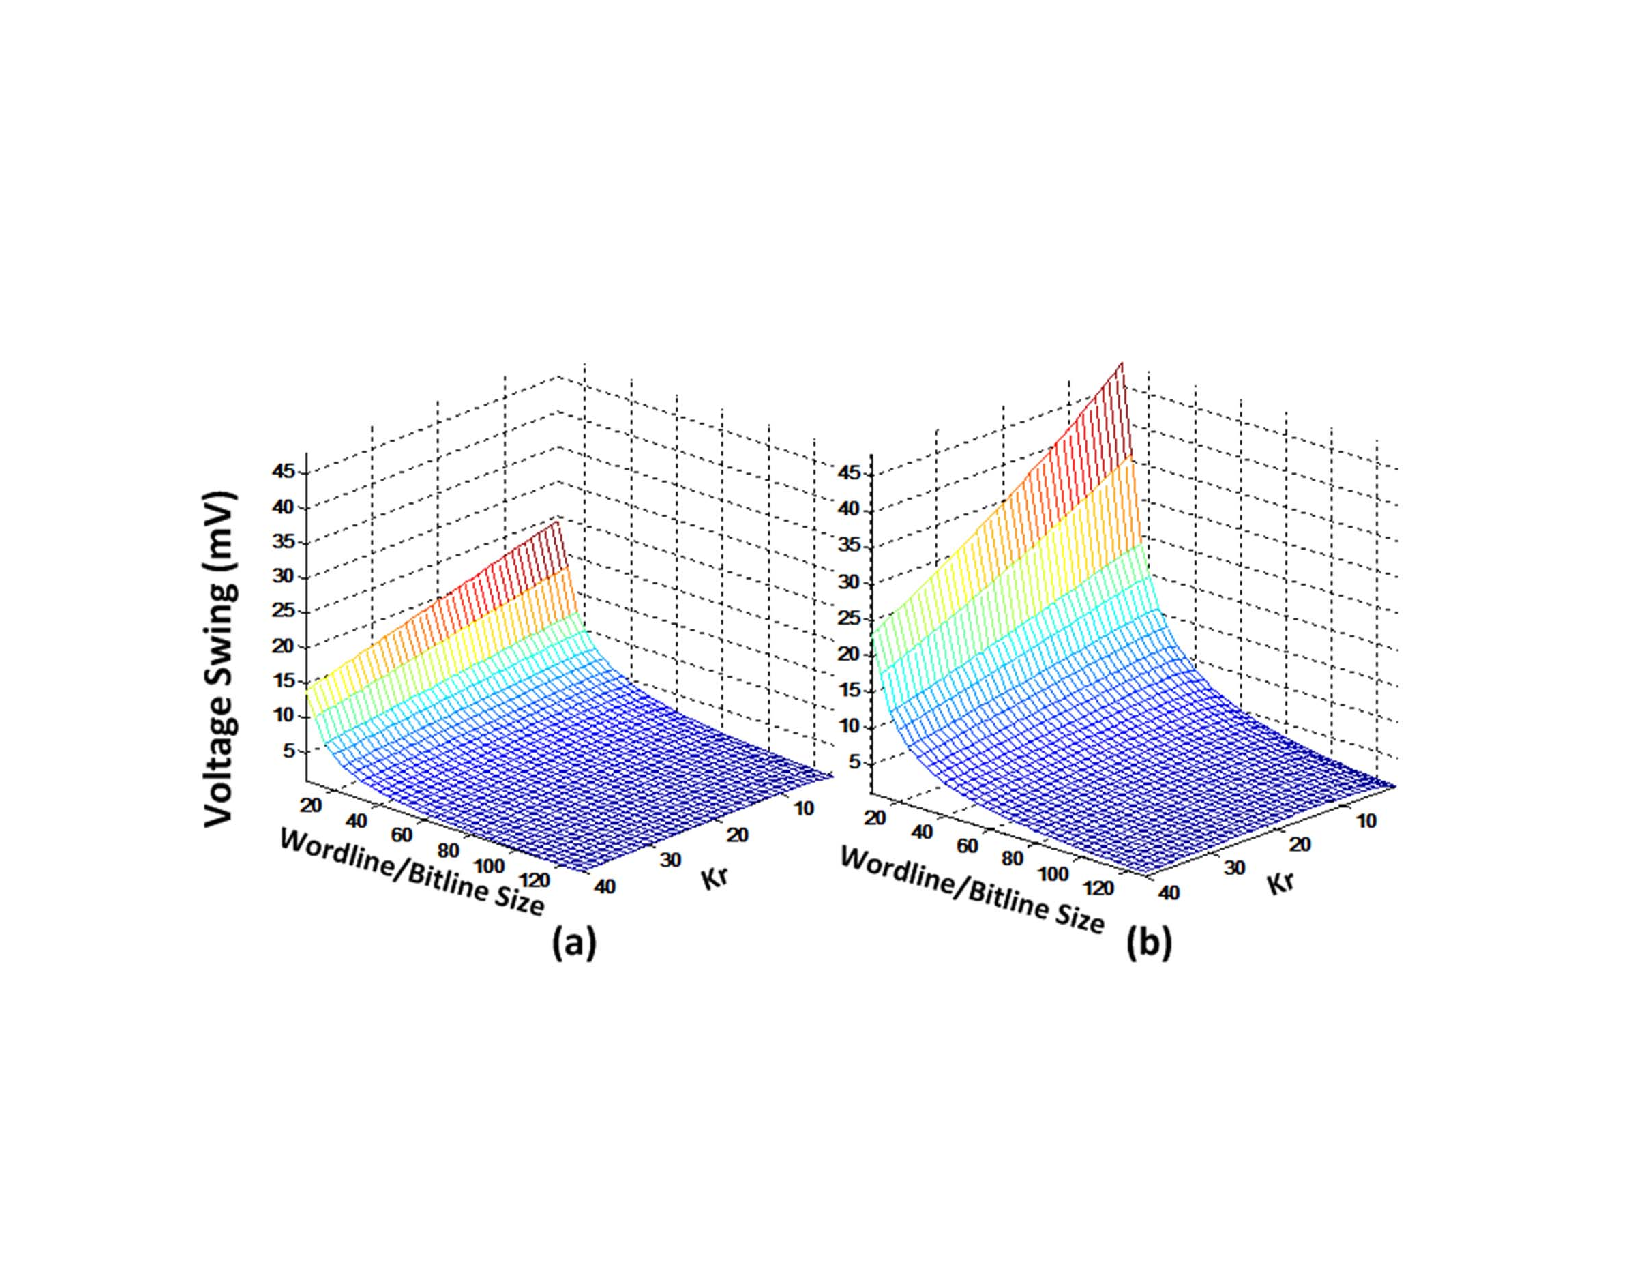
\includegraphics[width=0.5\textwidth]{./figures/sense_margin_f}\\
%  \caption{Relationships among the voltage swing, array size and non-linearity. (a) Normal sensing scheme; (b) Two-step sensing scheme}\label{fig:sense_margin}
%\end{figure}

%\vspace{10pt}
\section{Non-linearity and Write Current Scaling}\label{sec:scale}
%\section{Non-linearity and Write Current Scaling}\label{sec:scale}
%\subsection{Non-linearity of the ReRAM Cell.} \vspace{6pt}
\begin{figure}[!b]
\centering
  % Requires \usepackage{graphicx}
  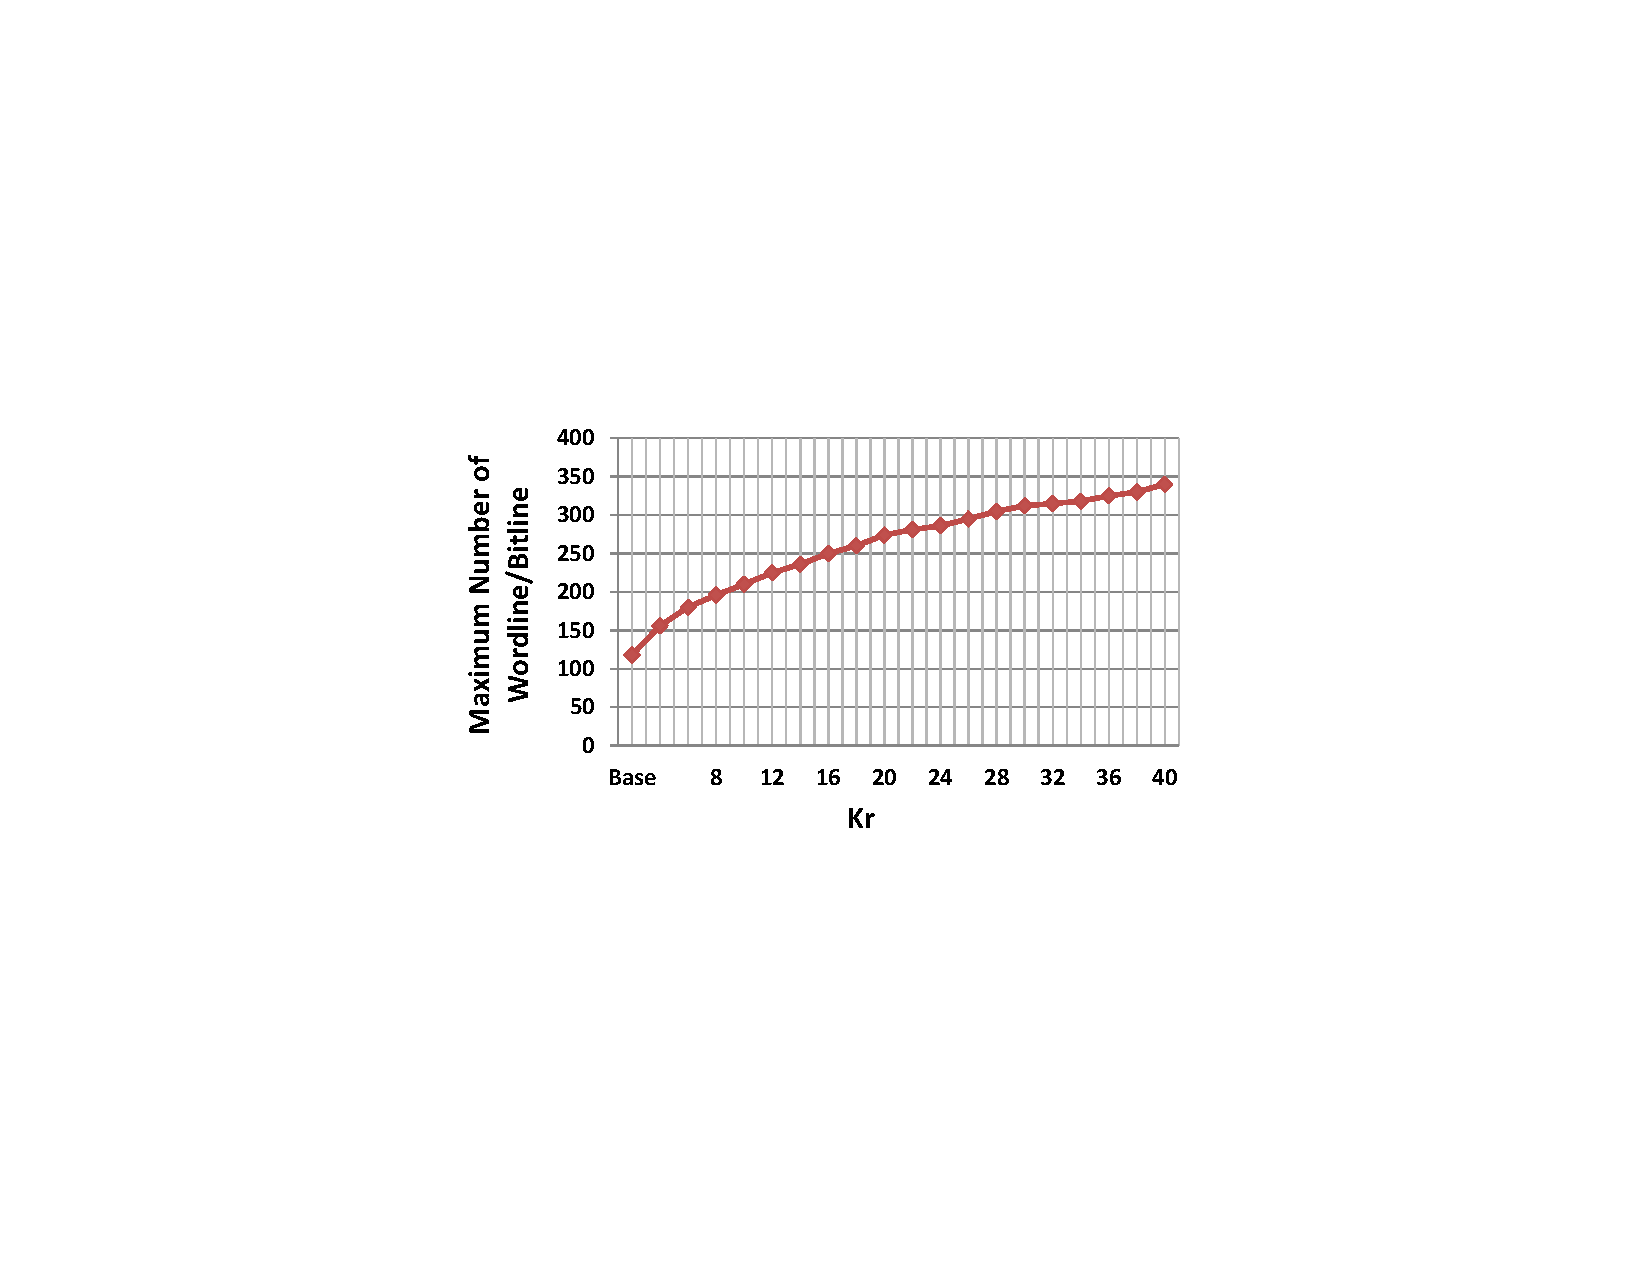
\includegraphics[width=0.45\textwidth]{./figures/non_linear_f}\\
  \caption{The maximum array size with different non-linearity coefficient.}\label{fig:non_linear}
\end{figure}
One of the most distinct features of ReRAM is its non-linearity. Normally,
the $K_r(p,V)$ value for memristor-based ReRAM is larger than 20, meaning
that the resistance of a half-biased cell is at least 10 times larger than
a full-biased cell. Clearly, the ReRAM cell with a larger non-linearity
coefficient results in a better memory cell since the current in the sneak
path will be significantly reduced. In addition, the increased resistance
at half-selected and unselected cells can also mitigate the voltage drop
along the activated wordline and bitline. Besides, we found that the
cross-point array design can also benefit from the scaling of the write
current. Figure~\ref{fig:non_linear} shows the influence of different
non-linearity coefficients and write current on the array size
requirements for one bit HWHB writing scheme. This figure shows that the array size limitation is relaxed as nonlinearity or write current scales. As we can tell from the figure, the maximum array size exceeds $1024\times 1024$ when we have a nonlinearity of $30$ together with a write current of $40\mu A$. 

\textbf{Moreover, the increase of non-linearity or scaling of write
current can also reduce the energy consumption and area overheads of the
cross-point array. As shown in Figure~\ref{fig:non_linear_energy}, for a
$512 \times 512$ array, the energy consumption for the write operation
decreases dramatically with the increase of non-linearity coefficient
$K_r$. As $K_r$ scales from 1 to 40, the write energy is reduced by
98.3\%. The driven current requirement is shown in
Figure~\ref{fig:area_all}(a), and the corresponding area overheads of the
voltage drivers are compared to the array size at
Figure~\ref{fig:area_all}(b). The baseline design is unacceptable because
the area of voltage drivers is about 11.6 times larger than the area of
the cross-point array. In this case, the area efficiency of ReRAM's $4F^2$
cell size will be offset by the extremely huge area overhead of the
voltage drivers. However, with the increase of non-linearity, the area of
voltage drivers becomes comparable to the array area. Therefore, we can
conclude that, the ReRAM cells with a small non-linearity coefficient are
not suitable for the cross-point structure based memory array. Next, we
study the area overhead of multi-bit write. Figure~\ref{fig:Area_kr20}
shows the normalized areas of the voltage drivers for one bit and
multi-bit write operations. As mentioned, multi-bit write operations
require larger driven current. Therefore, the area of voltage drivers for
multi-bit write operations are much larger than that for one bit write
operations. Finally, normalized areas of the one bit and multi-bit write
operations have opposite trends as the array size increases. Normalized
area for one bit write operation increases with the array size. On the
contrary, normalized area for multi-bit write decreases as the array size
increase.}

\begin{figure}%[!t]
\centering
  % Requires \usepackage{graphicx}
  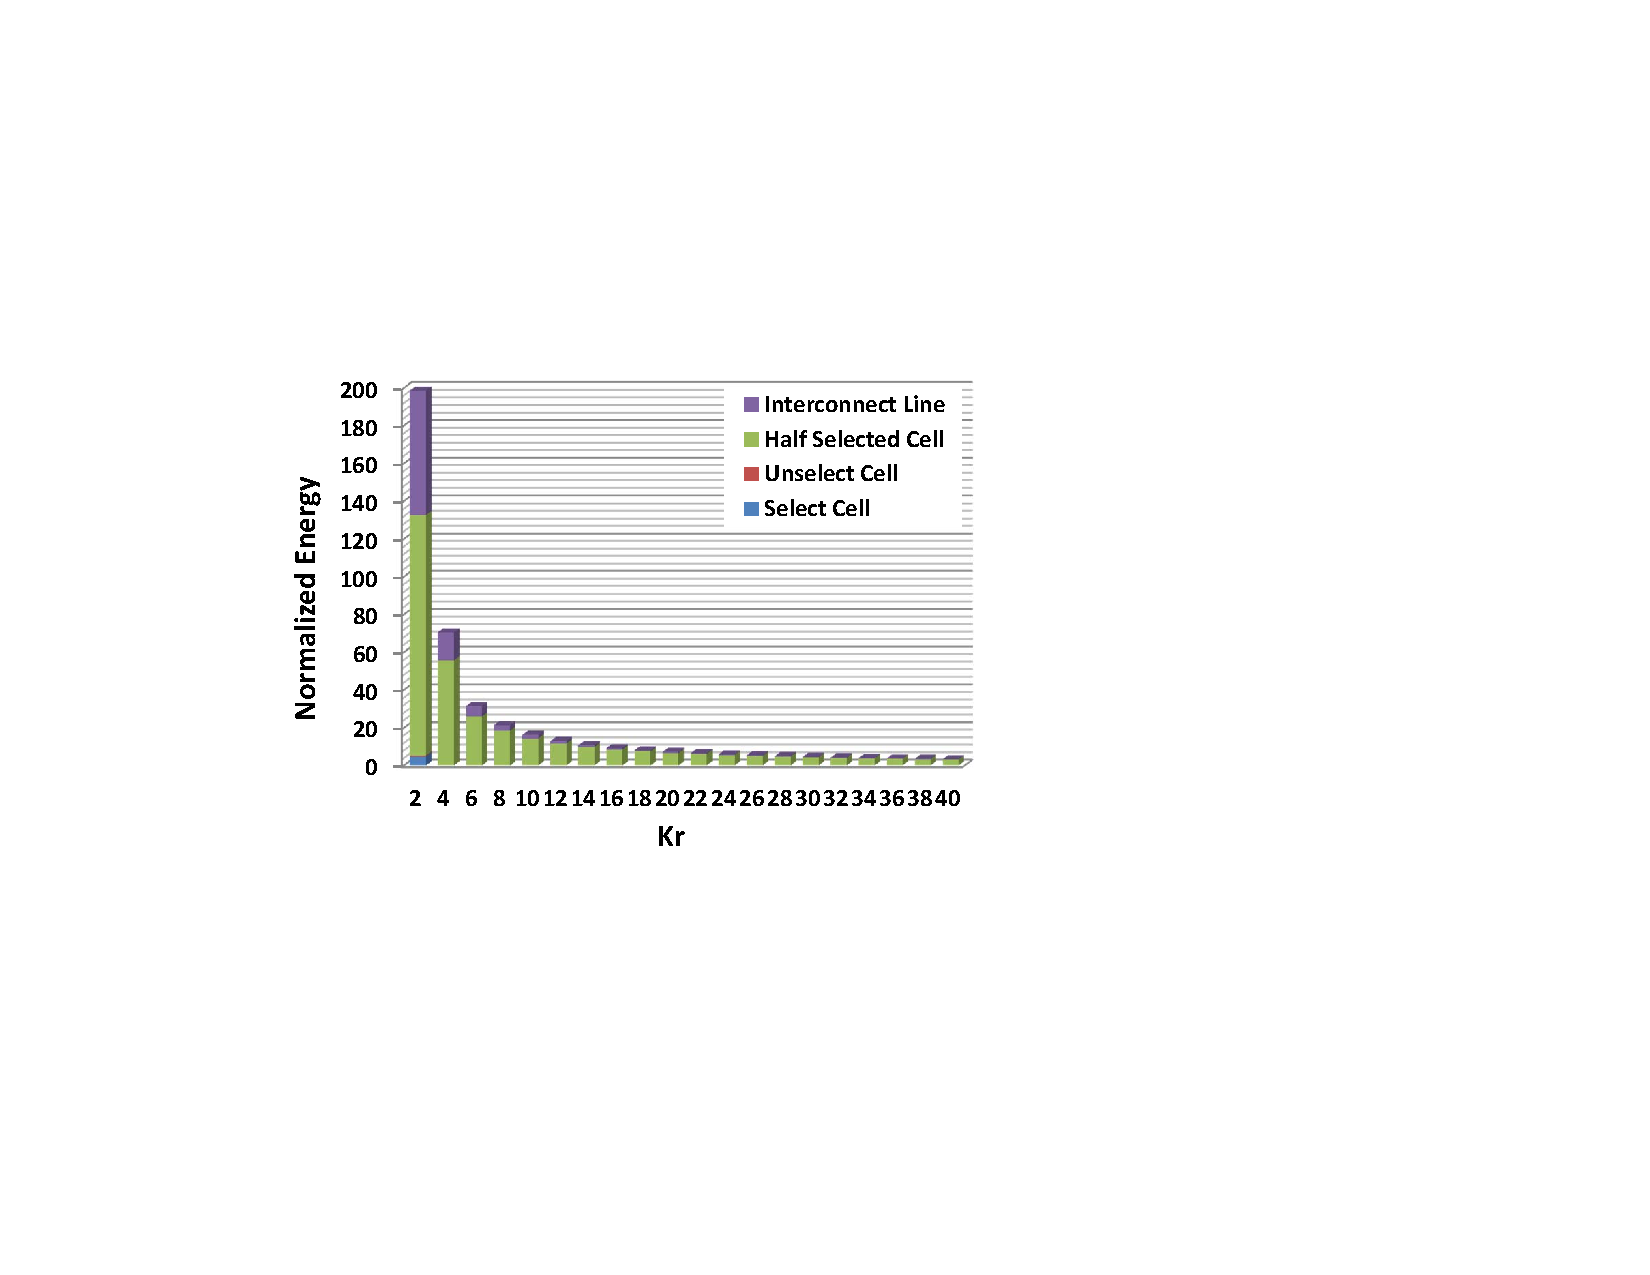
\includegraphics[width=0.38\textwidth]{./figures/non_linear_energy.pdf}\\
  \caption{The normalized energy consumption with non-linear ReRAM cells.}\label{fig:non_linear_energy}
\end{figure}

%\begin{figure}%[!t]
%\centering
%  % Requires \usepackage{graphicx}
%  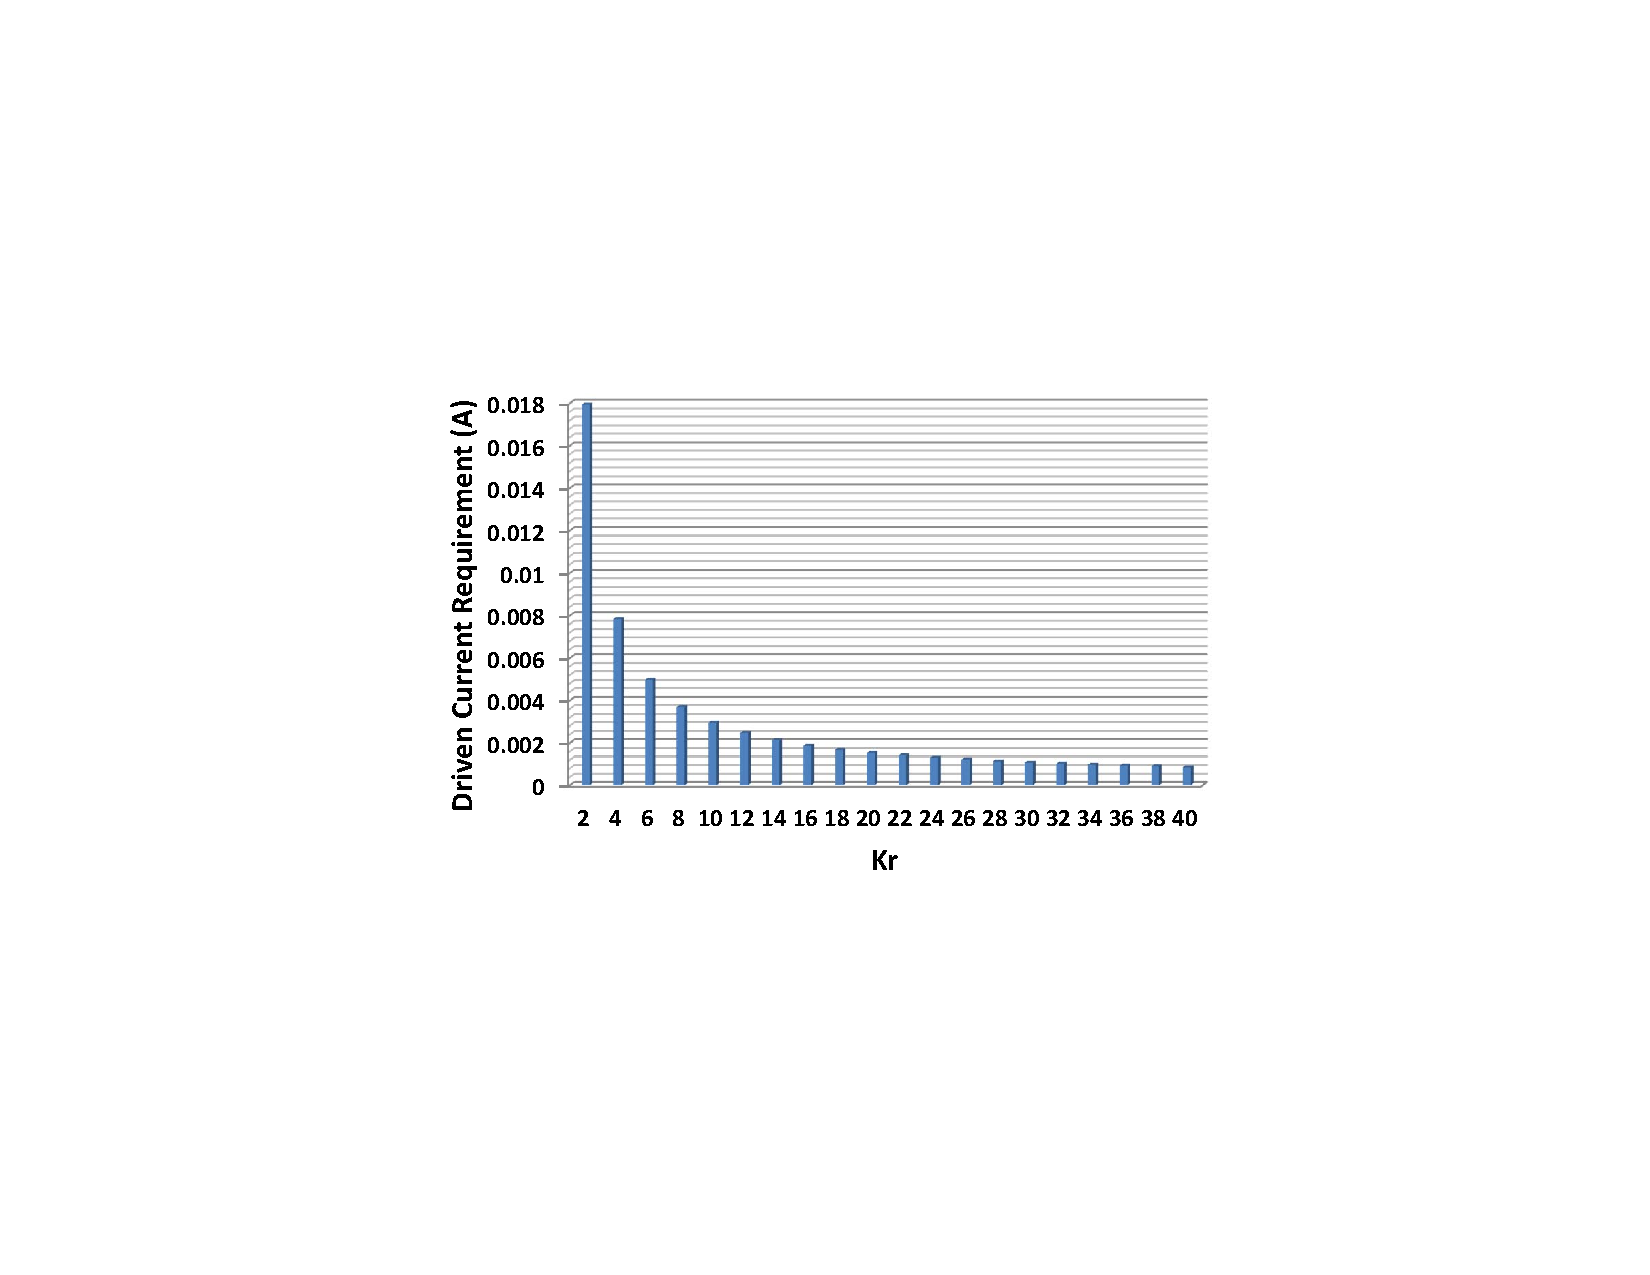
\includegraphics[width=0.4\textwidth]{./figures/non_linear_I.pdf}\\
%  \caption{The}\label{fig:non_linear_I}
%\end{figure}
%
%\begin{figure}%[!t]
%\centering
%  % Requires \usepackage{graphicx}
%  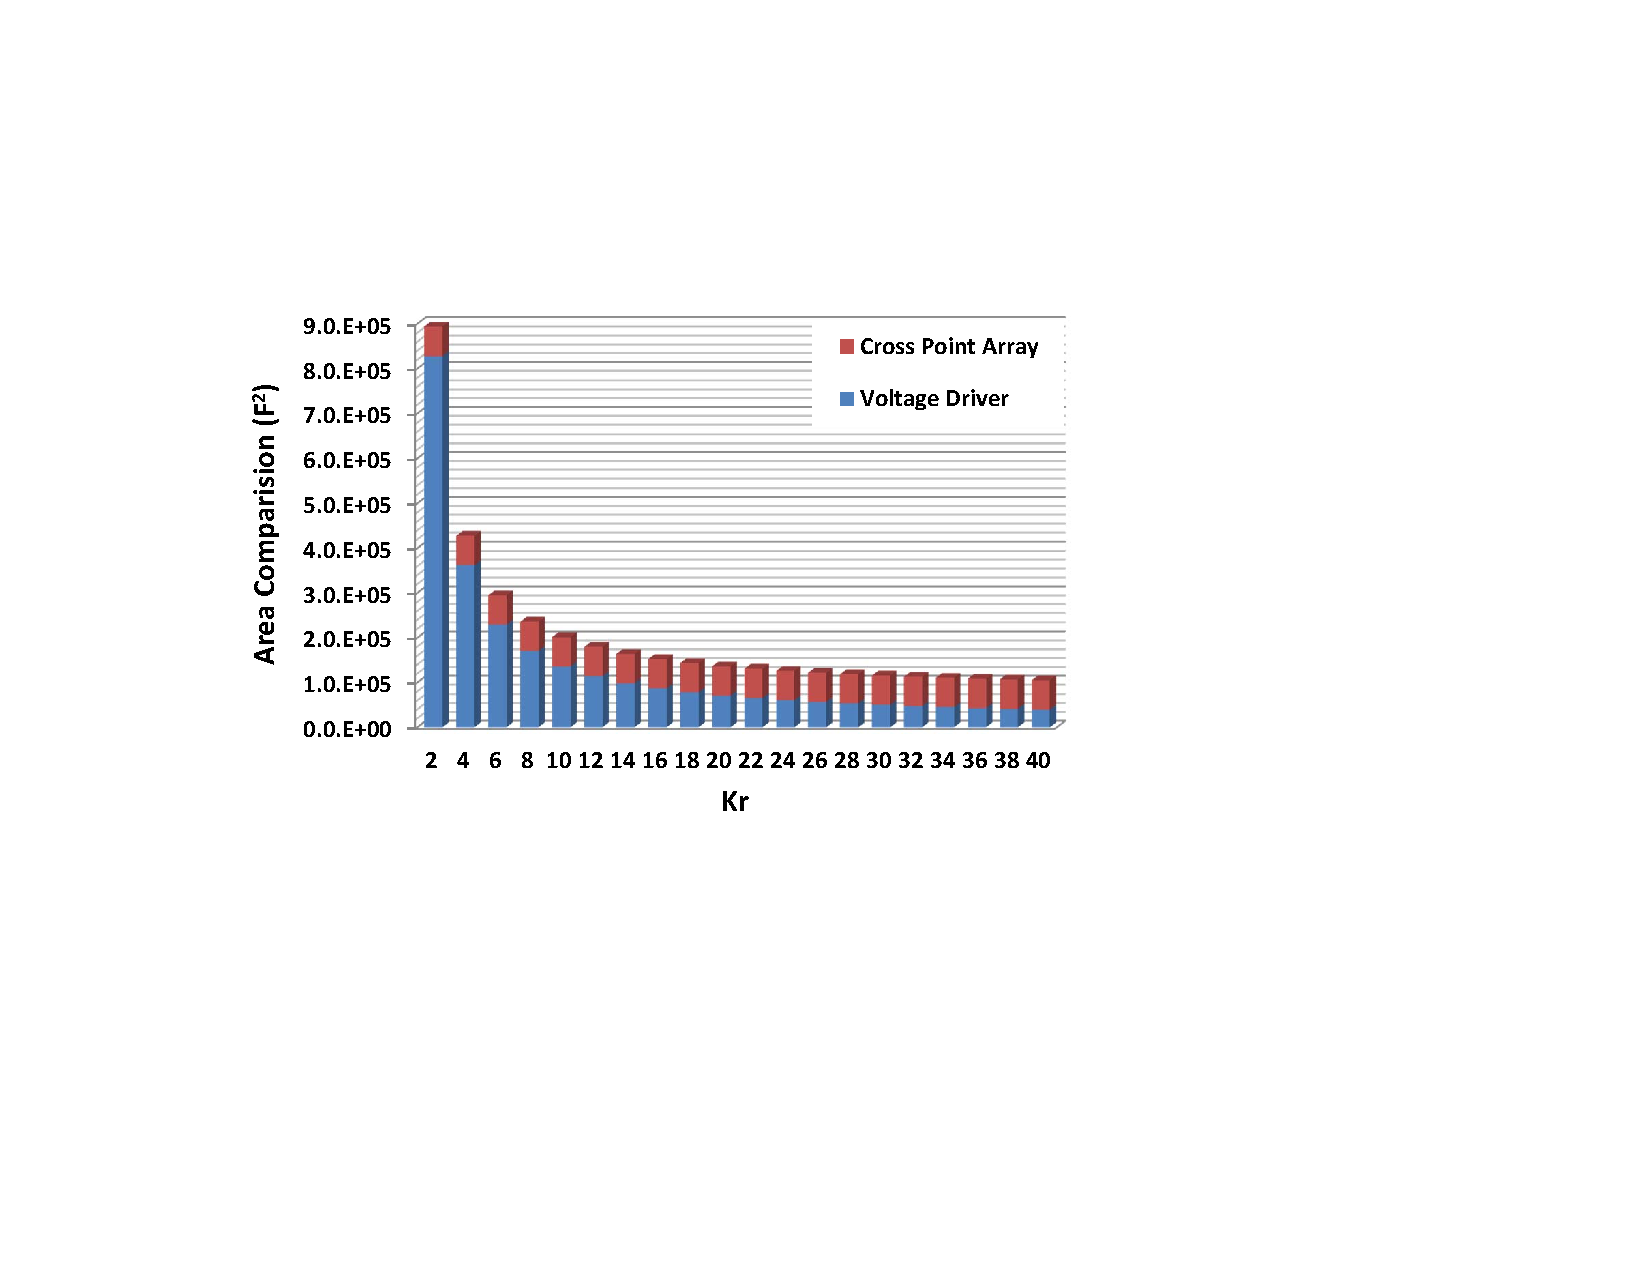
\includegraphics[width=0.4\textwidth]{./figures/non_linear_ara.pdf}\\
%  \caption{The}\label{fig:non_linear_ara}
%\end{figure}
\begin{figure}%[!t]
\centering
  % Requires \usepackage{graphicx}
  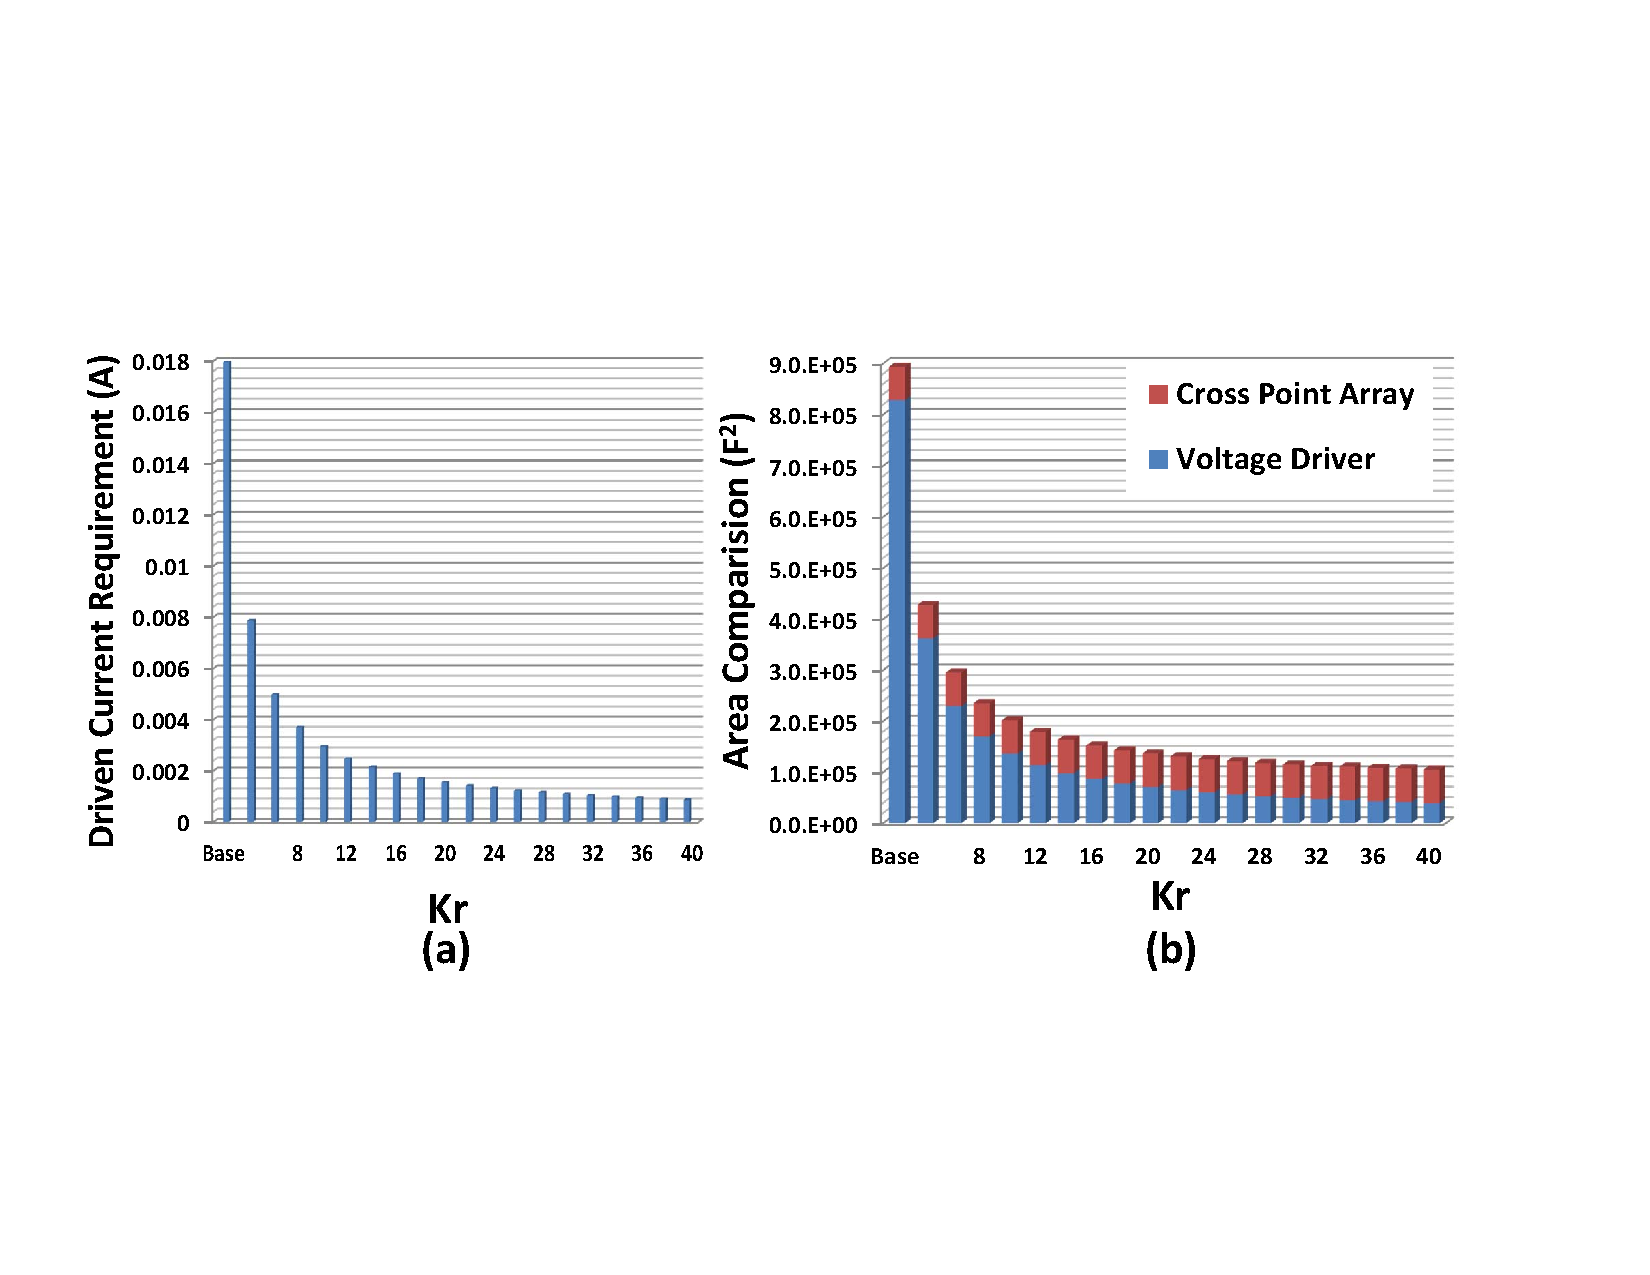
\includegraphics[width=0.5\textwidth]{./figures/area_all.pdf}\\
  \vspace{-5pt}
  \caption{The driven current requirements and area overheads with different non-linearity coefficients}\label{fig:area_all}
 \vspace{-15pt}
\end{figure}


%\begin{figure}%[!t]
%\centering
%  % Requires \usepackage{graphicx}
%  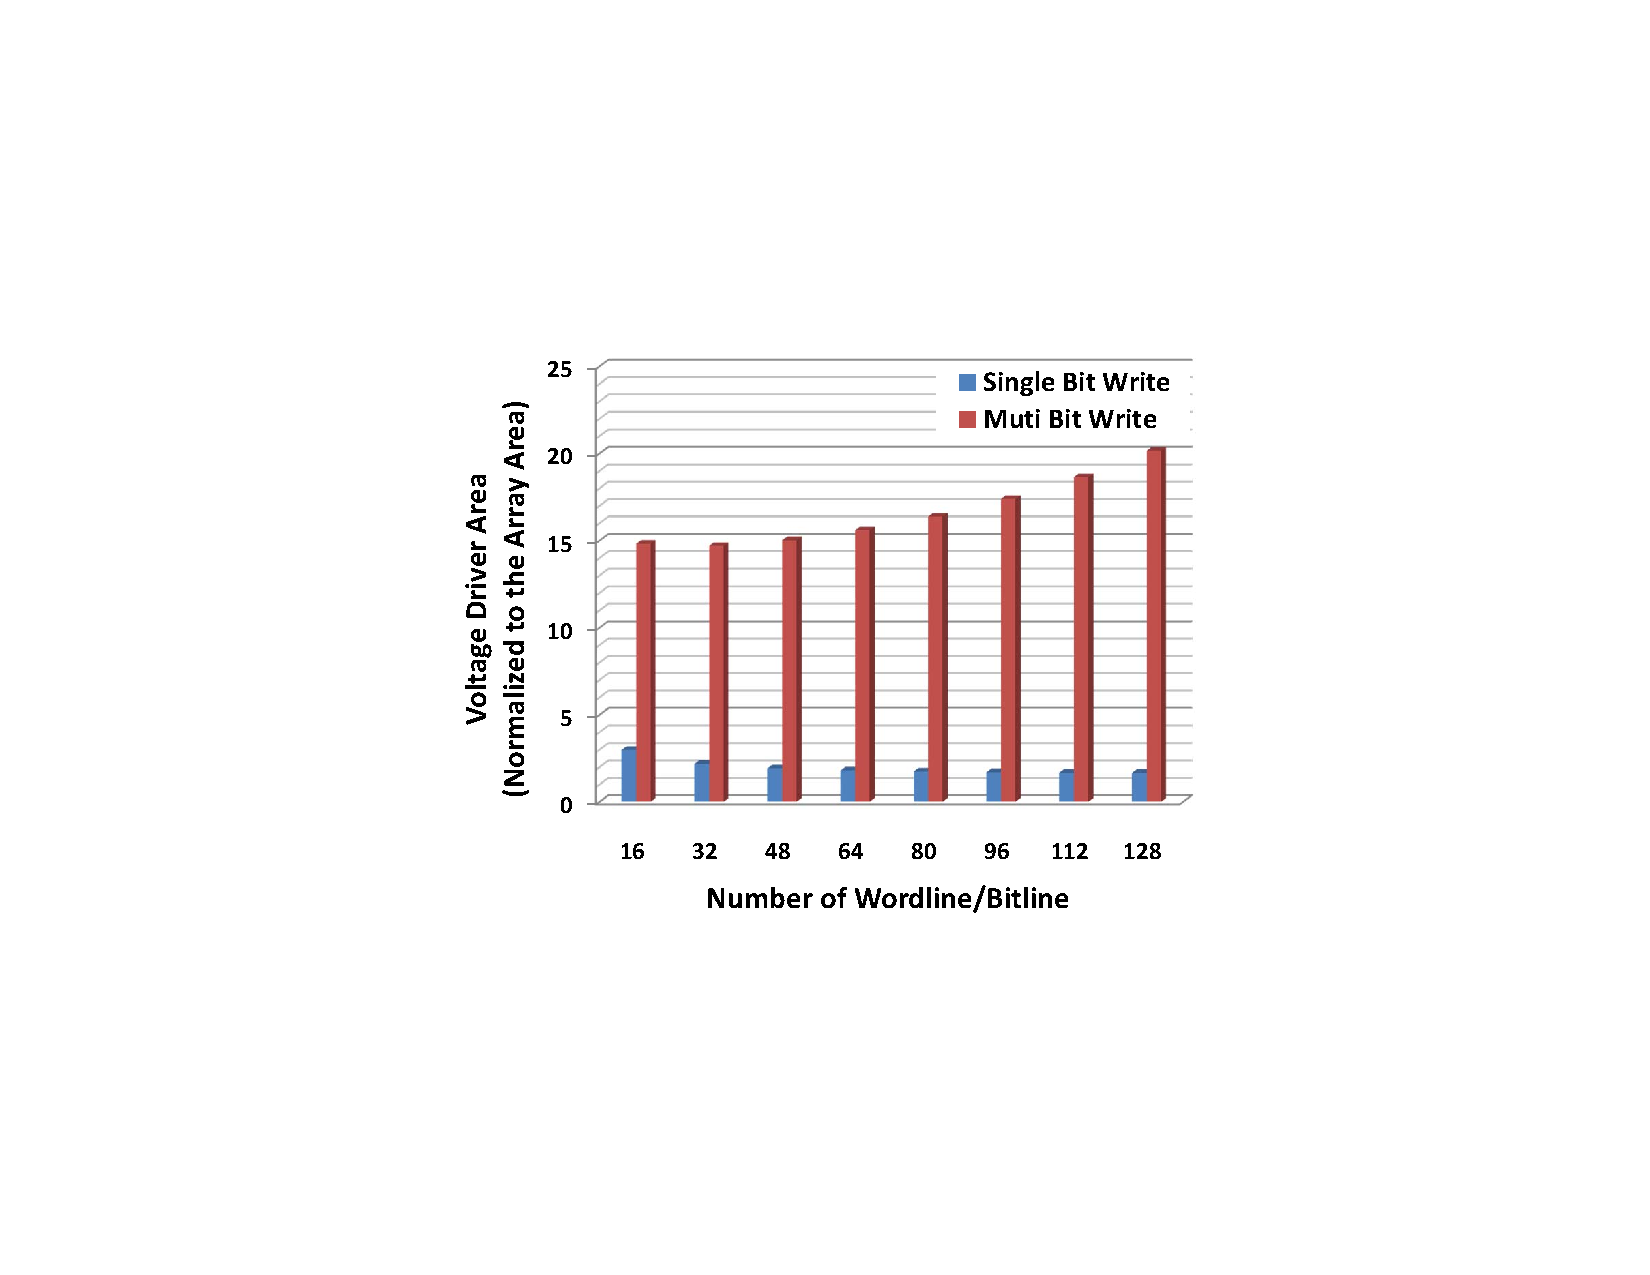
\includegraphics[width=0.35\textwidth]{./figures/Area_kr20_f.pdf}\\
%  \caption{The normalized area overhead of voltage drivers ($K_r=20$, the areas are normalized to the area of cross-point array). }\label{fig:Area_kr20}
%\end{figure}


Different from write operation, the read operation can not benefit from
the increasing of non-linearity or the scaling of write current.
Figure~\ref{fig:sense_margin} (a) shows the voltage swing with different
$K_r$ values and write current. Large non-linearity and small write
current are harmful to the voltage swing: \textbf{add discussion here
after we got the data}
%the non-linearity increases the resistance of half LRS and therefore the
%resistance difference between HRS and LRS cells is reduced; on the other
%hand, .
\begin{figure}[!t]
\centering
  % Requires \usepackage{graphicx}
  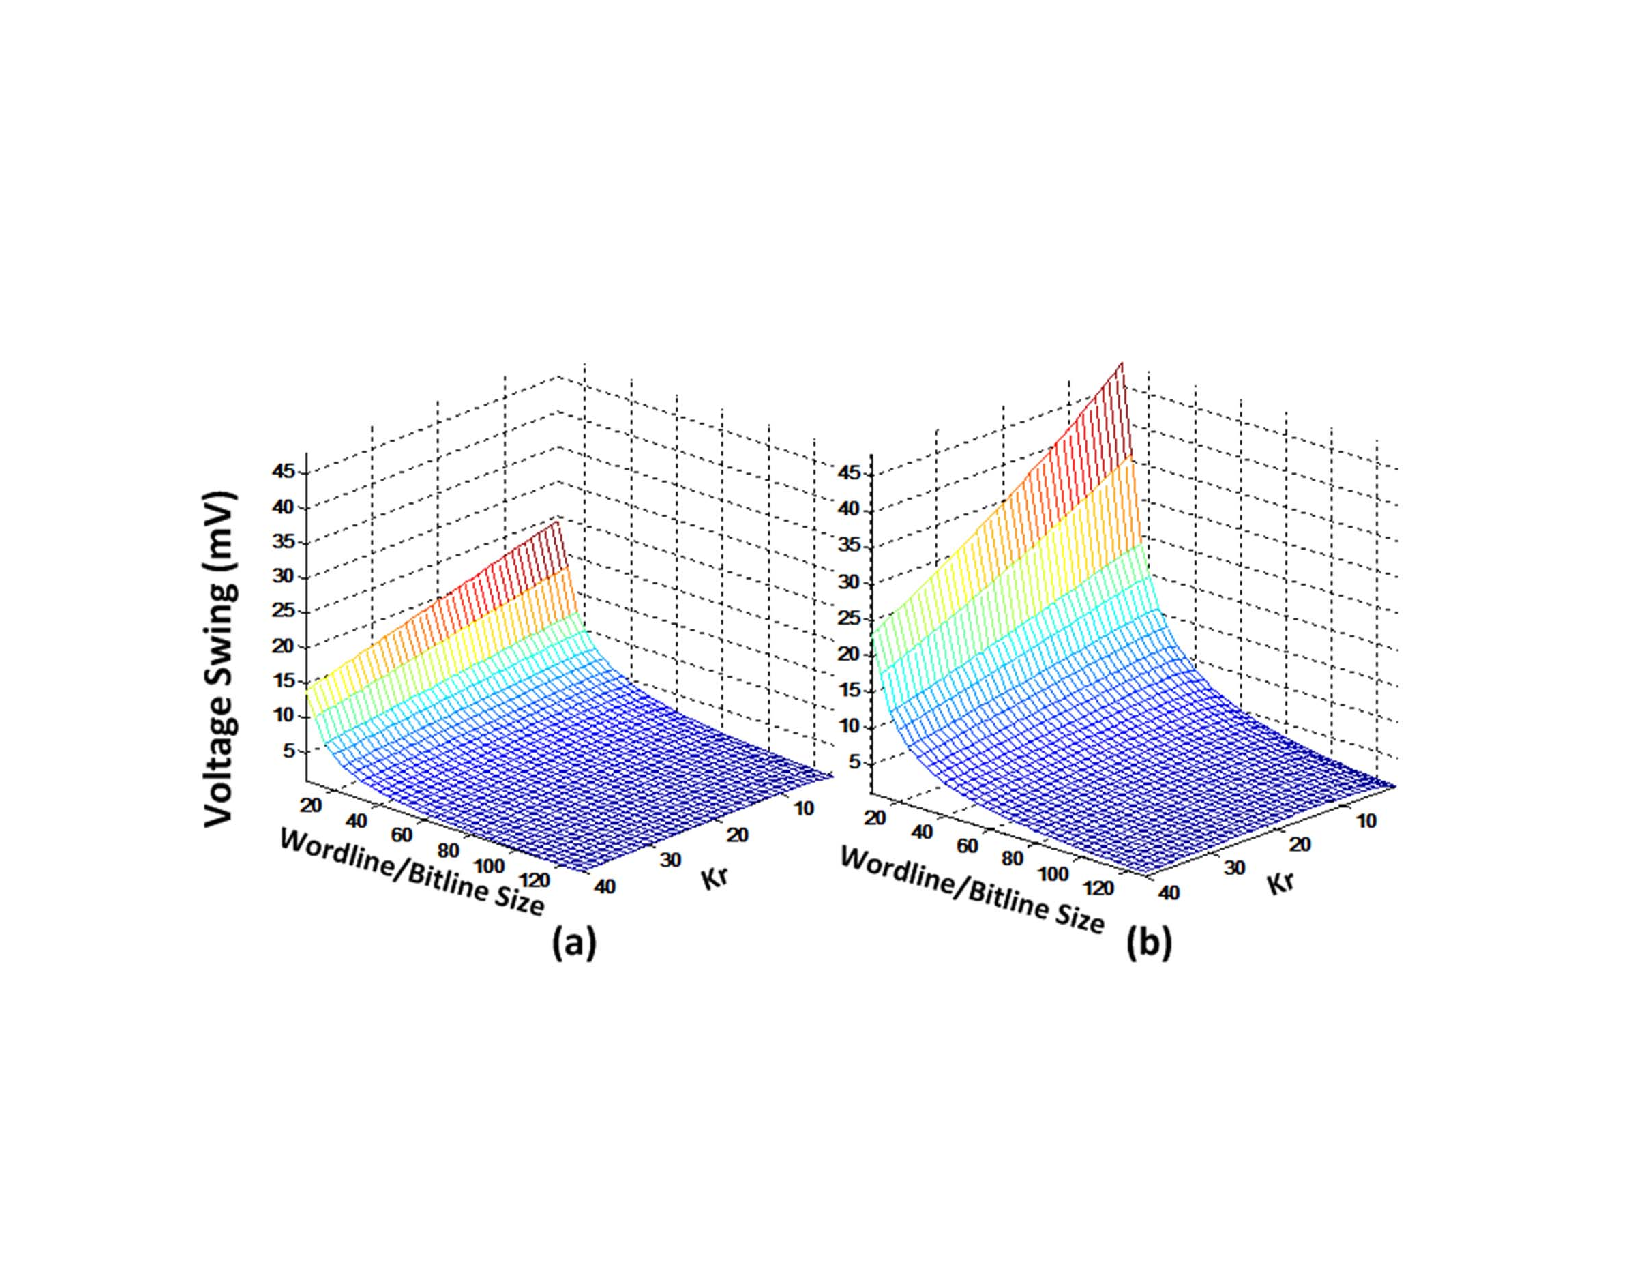
\includegraphics[width=0.5\textwidth]{./figures/sense_margin_f}\\
  \caption{Relationships among the voltage swing, array size and non-linearity. (a) Normal sensing scheme; (b) Two-step sensing scheme}\label{fig:sense_margin}
\end{figure}



%\subsection{Read Operation}
%In this section we applied the similar sensing scheme as
%\cite{crossbar_TED_2010} and \cite{crossbar_NANO08_Flocke}. In order to
%read cell $R_{i,j}$, the $i^{th}$ wordline is biased at $V_{READ}$ and all
%of the other wordlines and bitlines are grounded. Then the state of the
%selected cell is read out by measuring the voltage across $R_s$. The
%energy consumption for read operation can be analyzed by the same way as
%that of the write operation. Since the read voltage is much smaller than
%write voltage, the read energy is expected at least one order smaller than
%write operation. Additionally, since the read voltage/current is much
%lower than the write, we believe that the voltage drivers can always
%provide enough current for the read operation if they meet the current
%requirement for write operation. Therefore, we can conclude that the area
%overhead of voltage drivers is determined by the write current. However,
%the reliability of read operation is different from the write operation.
%The read reliability is determined by the voltage swing for reading HRS
%and LRS cells. Figure~\ref{fig:sense_margin} (a) shows the voltage swing
%with different array sizes and $K_r$ values. Large array sizes and large
%non-linearity are harmful to the voltage swing: on the one hand, a larger
%array has more sneak paths, making the output voltage very sensitive to
%the data pattern of unselected cells; on the other hand, the non-linearity
%increases the resistance of LRS and therefore the resistance difference
%between HRS and LRS cells is reduced. In order to improve the reliability
%of the read operation, a two-step sensing scheme can be applied, which
%senses the current of an unselected cell first, then the overall current
%is sensed, and after that the current difference is converted to the
%output voltage. The voltage swing of this two-step sensing scheme is shown
%in Figure~\ref{fig:sense_margin} (b). By using this two-step sensing
%schemes, the voltage swing for a given array size and non-linearity
%coefficient is doubled.
%
%
%
%\begin{figure}[!t]
%\centering
%  % Requires \usepackage{graphicx}
%  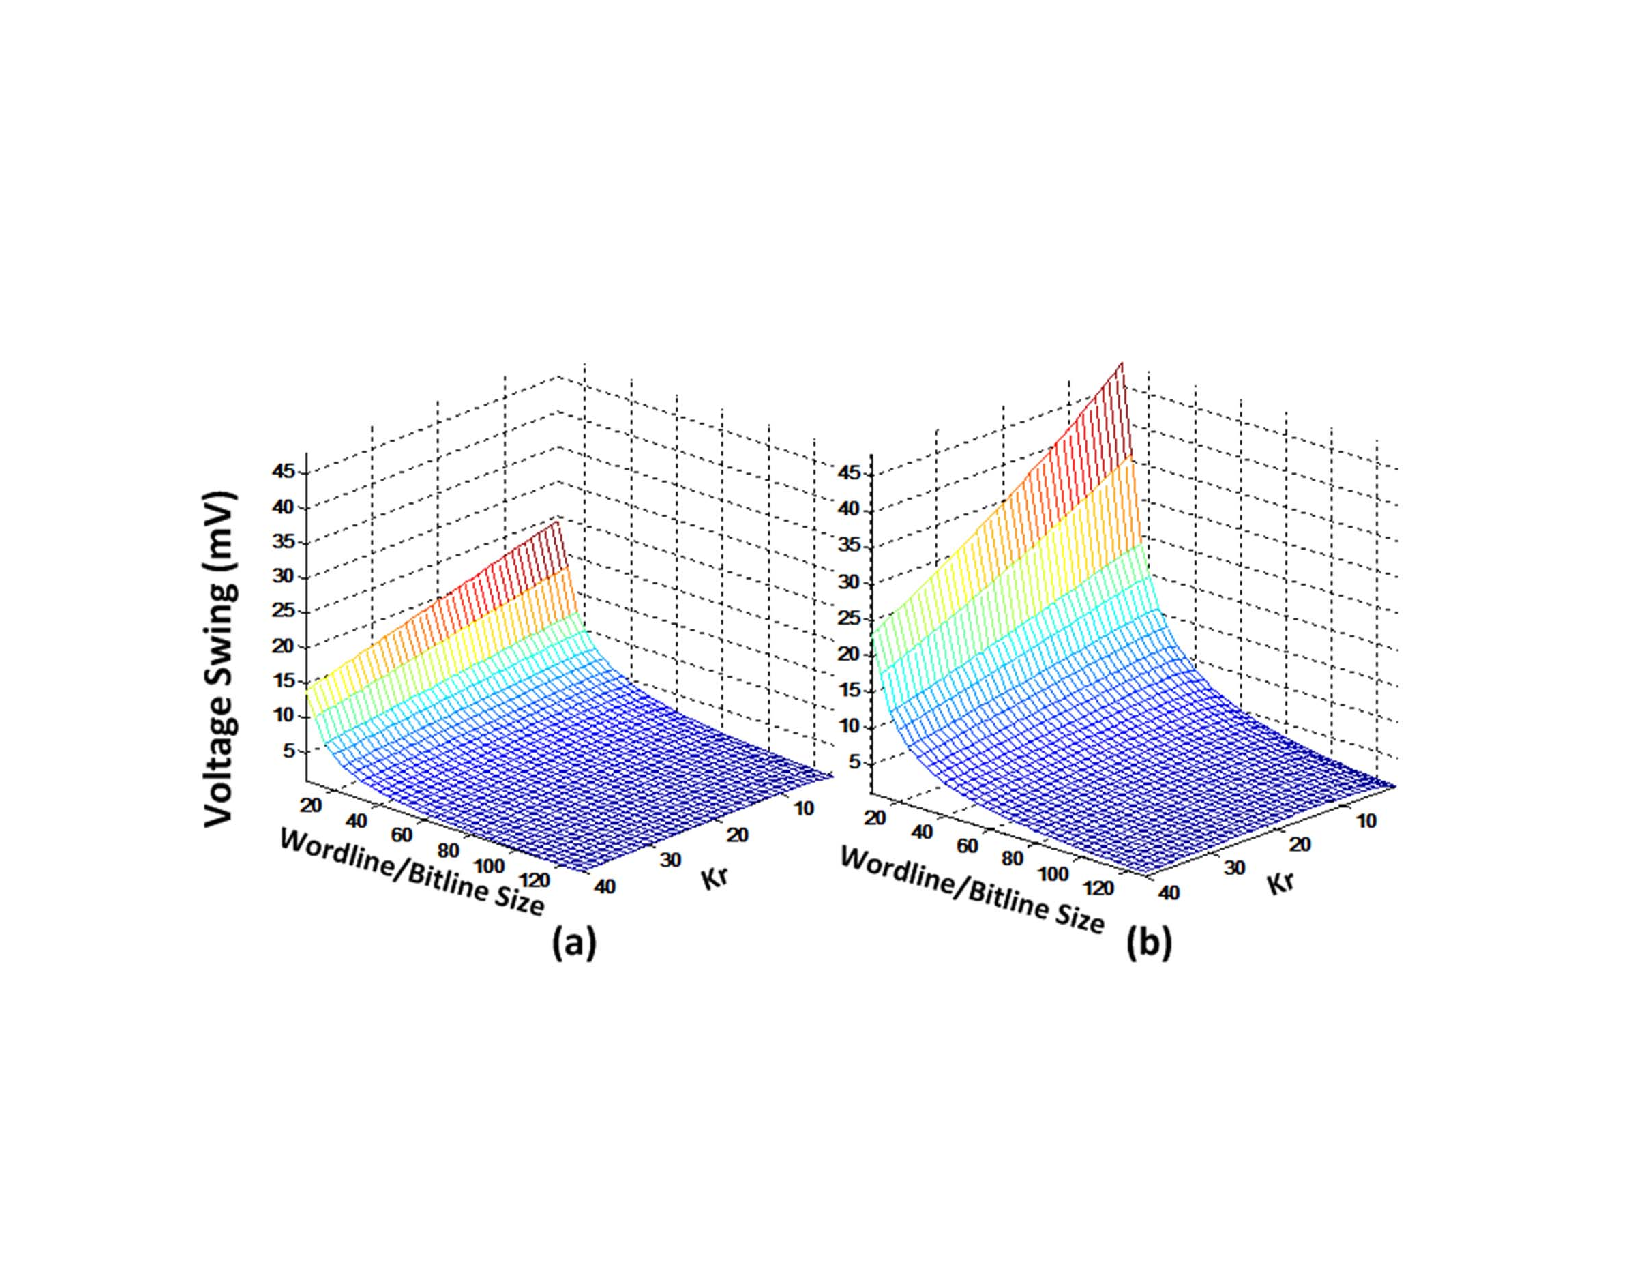
\includegraphics[width=0.5\textwidth]{./figures/sense_margin_f}\\
%  \caption{Relationships among the voltage swing, array size and non-linearity. (a) Normal sensing scheme; (b) Two-step sensing scheme}\label{fig:sense_margin}
%\end{figure}

%\vspace{10pt}
\section{Design Methodology}\label{sec:framwork}
Based on the analysis of Section~\ref{sec:w_and_r}, a new design flow is proposed to explore the design space of cross-point ReRAM arrays, as shown in Figure~\ref{fig:FlowChart}. Generally, the flow can be summarized as two stages: initialization stage and computation stage. At the initialization stage, the physical parameters, including the resistances of ReRAM cell, interconnect wires, and pull up resistors, the threshold voltage of the ReRAM cell, as well as non-linearity coefficients, are initialized. Since these values are constant for a given process technology, they need not be changed during the design space exploration. As a next step, the design constraints are specified based on area/energy budgets and different applications. Then the  original version of coefficients matrix $A_{basic}$ and the vector of constant terms $C_{basic}$ are set up. Since the value of $A_{basic}$ and $C_{basic}$ do not consider the edge conditions of the write/read schemes and their values do not change during the design space exploration. Then the programming schemes are chosen. The designer can either explore all possible programming schemes or choose a specific scheme based on previous results (for example, we have already shown that one bit write operation is more suitable for an area-constrained design than multi bit write). Then the final step of the initialization stage is to adjust the coefficients in $A_{basic}$ and $C_{basic}$ based on the edge conditions. At the beginning of the computing stage, the reliable array size is obtained by examining the worst case voltage drop and the read margin requirement. Then an iteration is performed to calculate the energy consumption and area overheads for each array size. The result are analyzed for all the array organizations. If there is any array organization that meets the design constraints provided at  the initialization stage, then the allowable array sizes with their energy consumption and area overheads are summarized as the design space for the given constraints. Otherwise, the programming schemes need to be adjusted for a new round of evaluation.



\begin{figure}[!t]
\centering
  % Requires \usepackage{graphicx}
  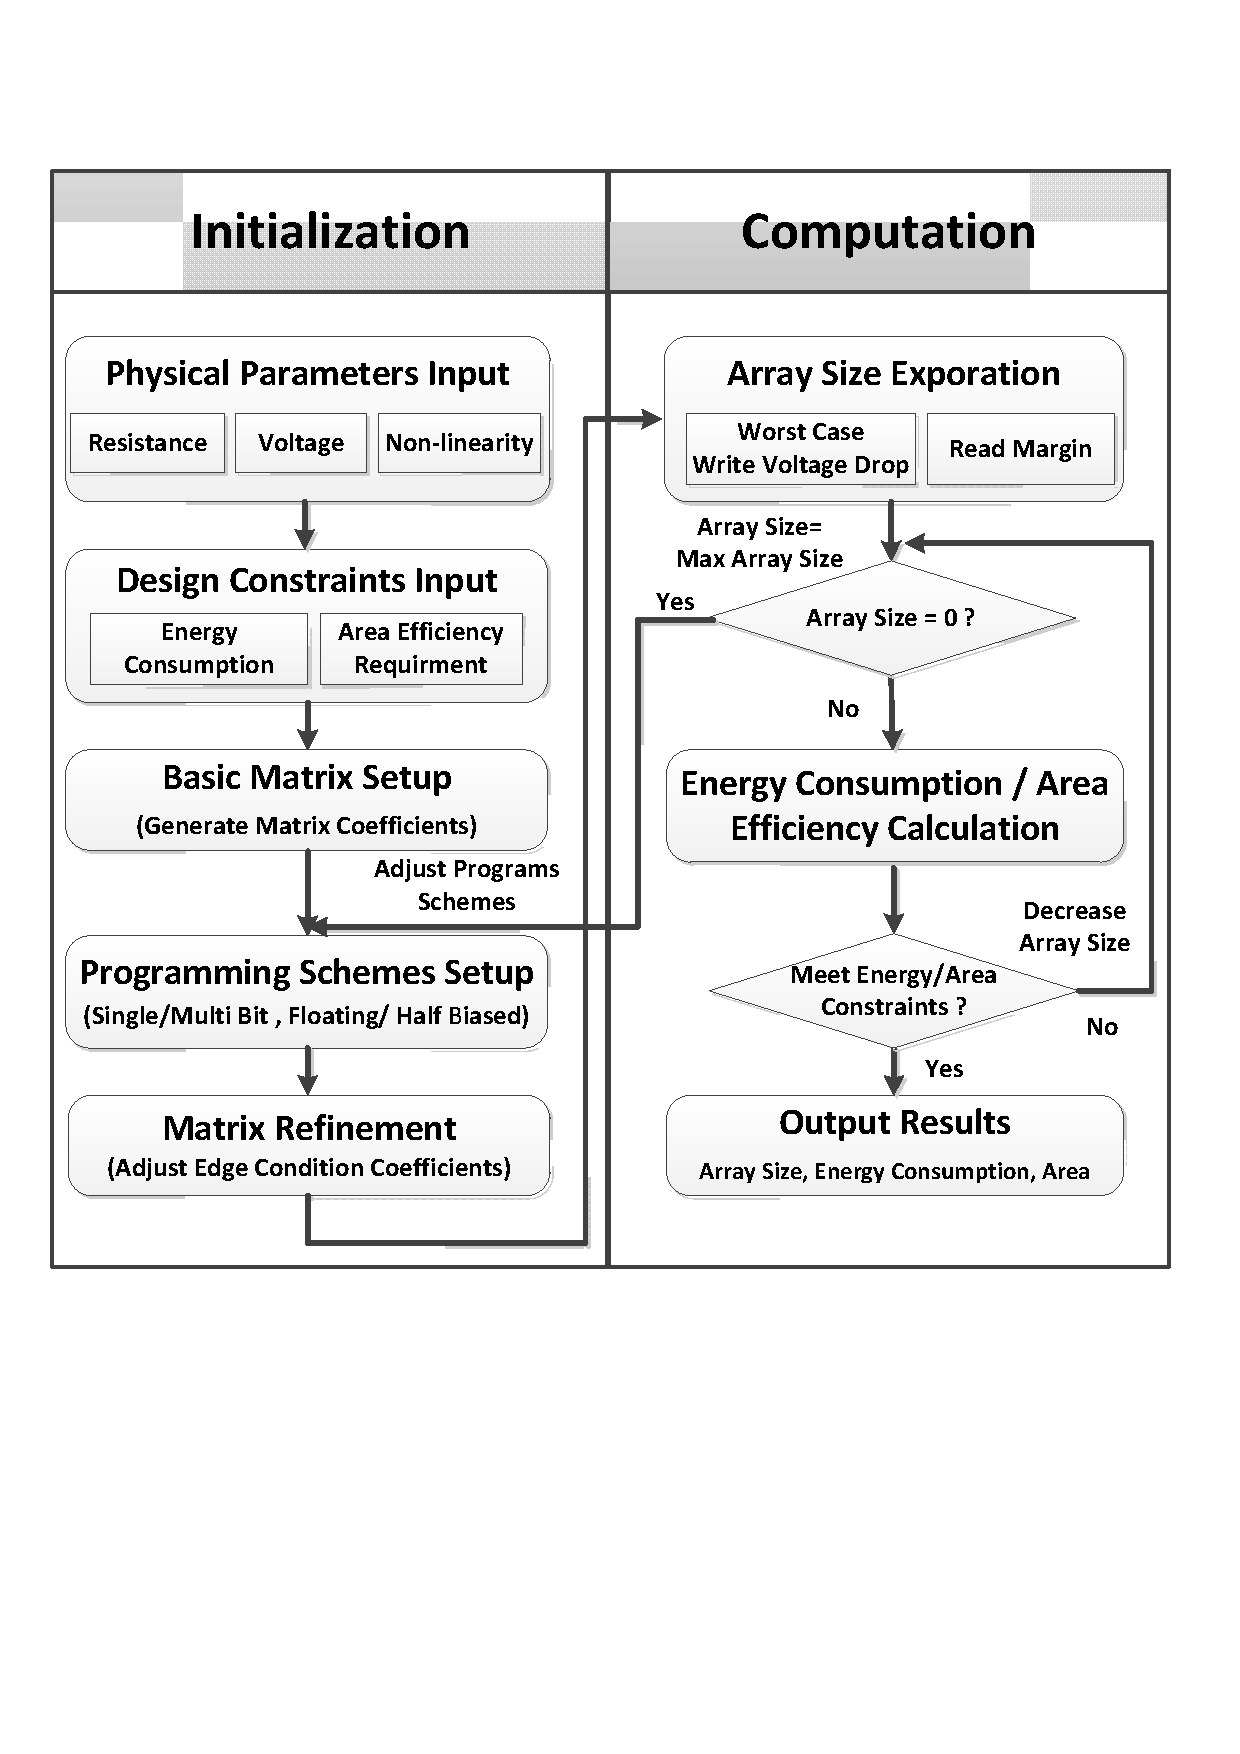
\includegraphics[width=0.5\textwidth]{./figures/FlowChart.pdf}\\
  \caption{The Proposed Design Flow of Design Space Exploration for ReRAM based Cross-point Array.}\label{fig:FlowChart}
  \vspace{-10pt}
\end{figure}

%\vspace{10pt}
\subsection{Experimental Results} \begin{figure}%[!t]
\centering
  % Requires \usepackage{graphicx}
  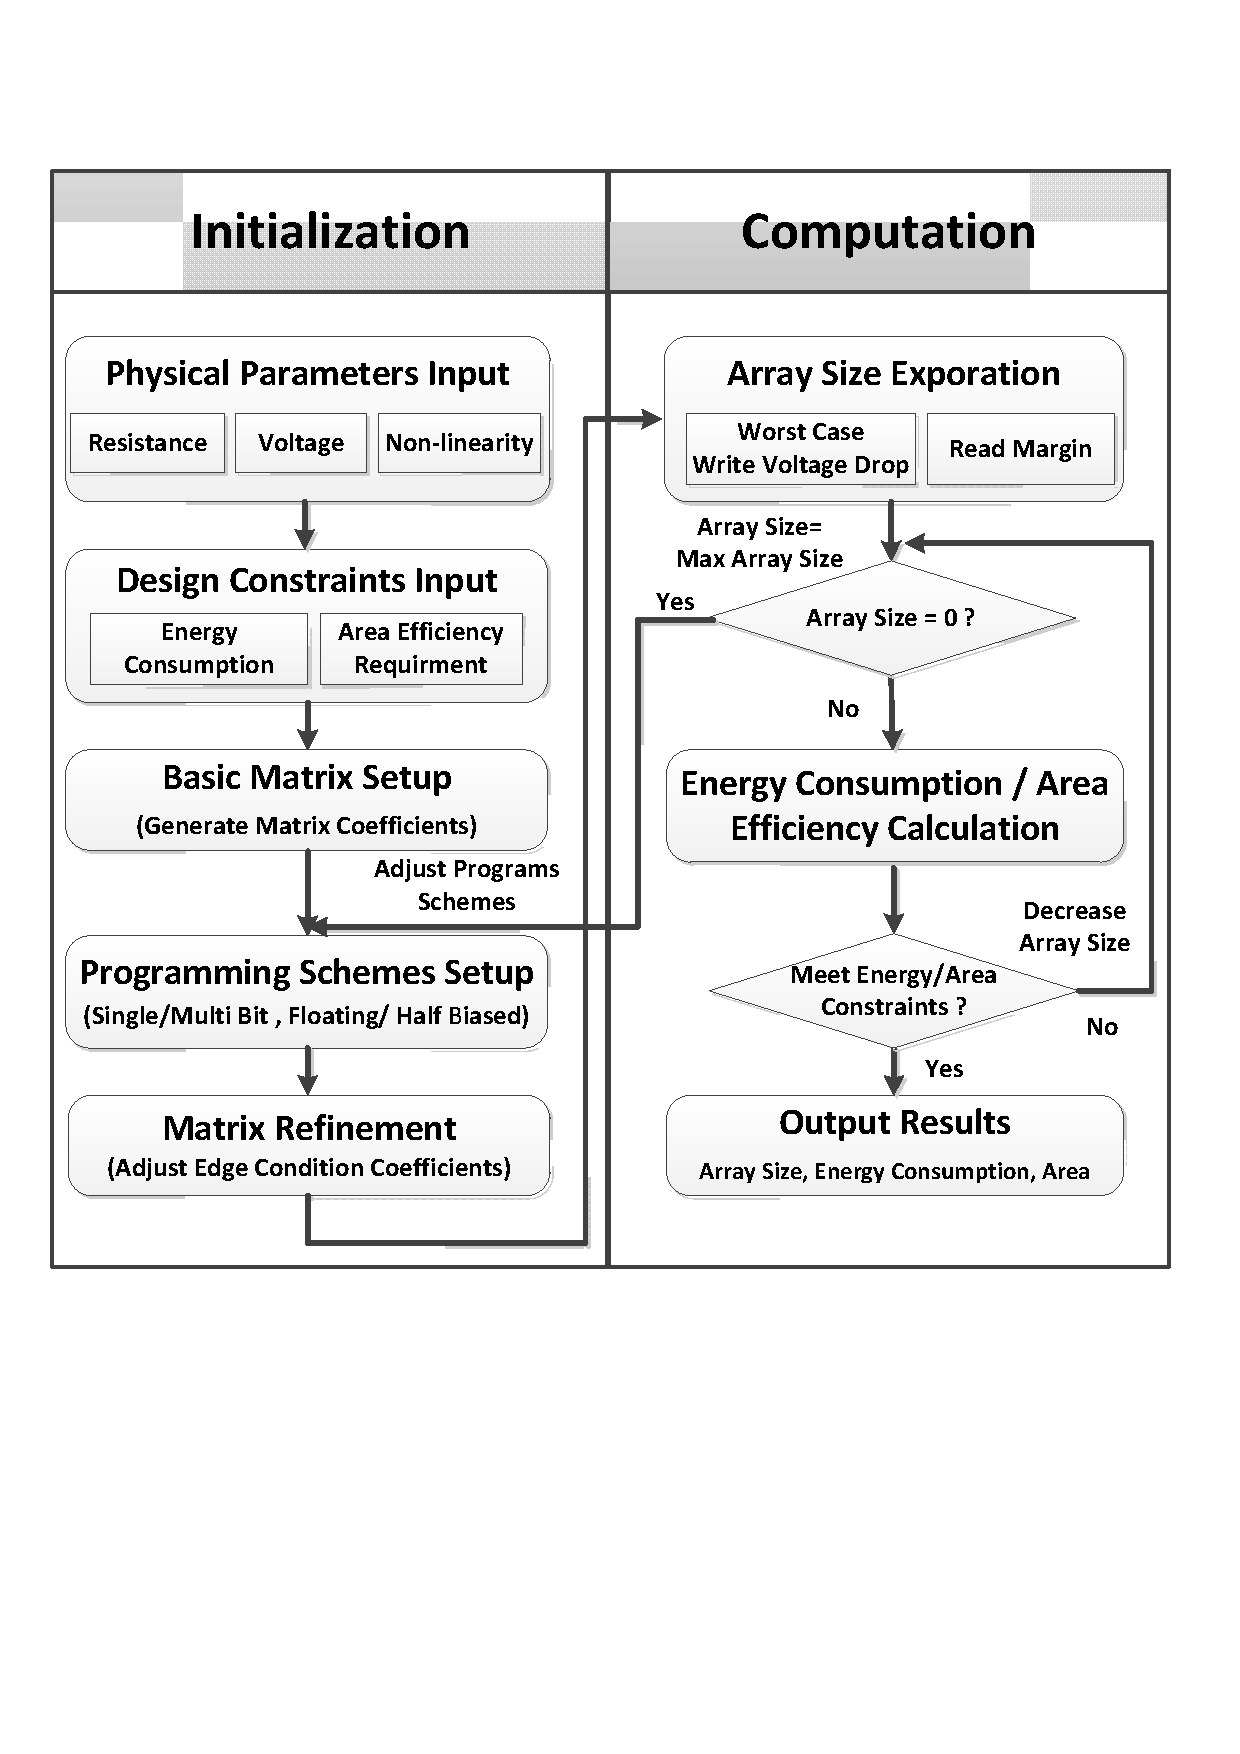
\includegraphics[width=0.5\textwidth]{./figures/FlowChart.pdf}\\
  \caption{The}\label{fig:non_linear_A}
\end{figure}
\vspace{10pt}
\subsection{Conclusion}
\appendix[Details of the Modeling of Cross-Point Array]
Test


%\begin{spacing}{0.9}
%\begin{scriptsize}
\bibliographystyle{ieeetran}
\bibliography{./bib/crossbar,./bib/memristor,./bib/mis,./bib/ReRAM}
%\end{spacing}
%\end{scriptsize}

\end{document}
